\documentclass[12pt,a4paper]{article}
\usepackage[utf8]{inputenc}
\usepackage[T2A]{fontenc}
\usepackage[russian]{babel}
\usepackage{amsmath}
\usepackage{amsfonts}
\usepackage{amssymb}
\usepackage{graphicx}
\usepackage{geometry}
\usepackage{indentfirst}
\usepackage{array}
\usepackage{float}
\usepackage{booktabs}
\usepackage{caption}
\usepackage{subcaption}
\usepackage{url}

\geometry{left=2.5cm, right=1.5cm, top=2cm, bottom=2cm}
\graphicspath{{photoes/}}

% заглушка для данных, которые ещё не получены
\newcommand{\pending}[1]{%
  \par\noindent\fbox{\parbox{0.96\linewidth}{\small\textit{Ожидаются данные: #1}}}\par}
\newcommand{\Nt}{\mathrm{N_2}}

\begin{document}

\begin{titlepage}
    \begin{center}
        \textbf{МОСКОВСКИЙ ФИЗИКО-ТЕХНИЧЕСКИЙ ИНСТИТУТ} \\
        \textbf{(НАЦИОНАЛЬНЫЙ ИССЛЕДОВАТЕЛЬСКИЙ УНИВЕРСИТЕТ)}
        \\[1cm]
        {\large Физтех-школа аэрокосмических технологий}
        \\[3.5cm]
        {\Huge \textbf{Генерация и исследование свойств низкотемпературной плазмы}}
        \\[0.5cm]
        {\large Лабораторная работа №\,19}
        \\[1.5cm]
        \begin{flushright}
            \begin{tabular}{l l}
                Ларькин Глеб & Б03-301 \\
                % Фамилия Имя & Б03-XXX \\
            \end{tabular}
        \end{flushright}
        \vfill
        {\large Долгопрудный, 2026 г.}
    \end{center}
\end{titlepage}

\tableofcontents
\newpage

% ===============================================================
\section{Введение}
% ===============================================================

\textbf{Плазма} --- частично или полностью ионизованный газ, в котором
плотности положительных и отрицательных зарядов практически одинаковы.
По температуре тяжёлых частиц плазму делят на высоко- и
\textbf{низкотемпературную} (НТП). В НТП температура электронов
$T_e \sim 1$--$10$~эВ много больше температуры тяжёлых частиц
($T_g \approx 300$--$400$~К), поэтому НТП, как правило,
\textbf{неравновесна}: горячие электроны и холодные активные частицы
(ионы, возбуждённые атомы и молекулы, осколки молекул).

В работе исследуются два способа получения неравновесной НТП
\textbf{субатмосферного (форвакуумного) давления} $P_m \sim 1$--$10$~Торр:
\begin{enumerate}
  \item \textbf{электронно-пучковая плазма} (ЭПП) --- ионизация газа
        инжекцией пучка быстрых электронов ($E_b = 30$~кэВ) в отсутствие
        внешних полей (часть~1);
  \item \textbf{высокочастотный ёмкостный (ВЧЕ) разряд} между
        плоскопараллельными электродами, $f = 13{,}56$~МГц (часть~2).
\end{enumerate}

\paragraph{Цель работы.}
Изучить закономерности энерговыделения концентрированного электронного
пучка в газе, заполняющем цилиндрический контейнер, а также поведение и
свойства ВЧЕ-разряда субатмосферного давления в зависимости от условий
его генерации.

\paragraph{Задачи.}
\begin{itemize}
  \item По фотографиям ЭПП в кварцевой трубке построить продольные
        профили свечения $B(z)$ для $\Nt$ и Ar при
        $P_m = 1;\ 2{,}5;\ 5$~Торр; выявить влияние давления и рода газа.
  \item Провести моделирование энерговыделения $Q(z)$ методом Монте-Карло
        (программа <<ДОЗА>>) и сравнить его с экспериментом.
  \item Построить профили свечения $I(L)$ ВЧЕ-разряда в чистом и
        техническом гелии; проанализировать переход $\alpha \to \gamma$,
        оценить соответствующее значение $P_m L$.
  \item Провести оптическую спектроскопию ВЧЕ-разряда: качественный
        состав плазмы, давление перехода от излучения He к излучению
        $\Nt$, доля примеси азота, оптическая прозрачность плазмы.
\end{itemize}

% ===============================================================
\section{Часть 1. Электронно-пучковая плазма}
% ===============================================================

\subsection{Теоретические сведения}

\subsubsection{Электронные пучки и их генерация}

\textbf{Электронный пучок} --- совокупность электронов с упорядоченным
однонаправленным движением; в работе это тонкий моноэнергетический
пучок с $E_b = 30$~кэВ (ток $I_b \sim 2$--$4$~мА). В методичке указано
$U = 28$~кВ; мы берём $E_b = 30$~кэВ по данным, сообщённым на занятии.
Разница в 7\% меняет пробег~\eqref{eq:range} на $\approx 12\%$ и на выводы
не влияет. Пучки формируются \textbf{электронными пушками}
--- вакуумными диодами или триодами (ускорителями прямого действия).
По механизму эмиссии электронов различают пушки
\begin{itemize}
  \item с \textbf{термоэмиссионным катодом} --- плотность тока даётся
        формулой Ричардсона--Дэшмана
        \begin{equation}
            j_\text{э} = A^* T^2 \exp\!\left(-\frac{e\varphi_0}{kT}\right);
            \label{eq:rich}
        \end{equation}
  \item с \textbf{плазменным эмиттером} --- электроны отбираются с
        поверхности плазмы газового разряда (полый катод, высоковольтный
        тлеющий разряд);
  \item с \textbf{автоэлектронной} (полевой) эмиссией и пушки Шоттки
        (требуют вакуума $10^{-7}$--$10^{-9}$~Торр).
\end{itemize}

В установке используется \textbf{триодная пушка с термокатодом из
гексаборида лантана} LaB$_6$: таблетка нагревается до $T \approx 1700$~К.
Работа выхода LaB$_6$ мала ($e\varphi_0 \approx 2{,}9$~эВ против
4,4~эВ у вольфрама) и стоит в экспоненте~\eqref{eq:rich}, что даёт большие
$j_\text{э}$ при умеренной температуре. LaB$_6$ химически активен,
поэтому пушка работает в высоком вакууме ($\sim 10^{-5}$~Торр), а катодный
узел охлаждается водой. Между катодом и анодом расположен управляющий
электрод (регулировка тока смещением $U_\text{упр}$), за анодом ---
электромагнитная фокусирующая и отклоняющая системы.

\subsubsection{Ввод пучка в плотный газ: выводные окна}\label{sec:windows}

Пушка работает при $10^{-5}$~Торр, а плазма генерируется при
$1$--$10$~Торр: нужен узел, пропускающий пучок, но удерживающий перепад
давления (рис.~\ref{fig:windows}):
\begin{itemize}
  \item \textbf{фольговое окно} --- тонкая (15--100~мкм) фольга Ti, Ta,
        реже Al или Be; пучок теряет в ней энергию и греет её;
  \item \textbf{шлюзовая система} с дифференциальной откачкой ---
        несколько камер с диафрагмами, требует точной проводки пучка;
  \item \textbf{газодинамическое окно} --- канал малого диаметра в
        графитовых вставках, прожигаемый самим пучком (используется в
        работе).
\end{itemize}

\begin{figure}[H]
  \centering
  \begin{subfigure}{0.31\linewidth}\centering
    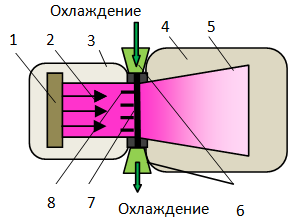
\includegraphics[width=\linewidth]{window_foil.png}\caption{фольговое}
  \end{subfigure}\hfill
  \begin{subfigure}{0.31\linewidth}\centering
    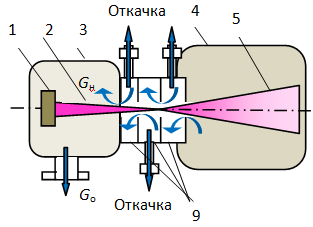
\includegraphics[width=\linewidth]{window_lock.png}\caption{шлюзовое}
  \end{subfigure}\hfill
  \begin{subfigure}{0.31\linewidth}\centering
    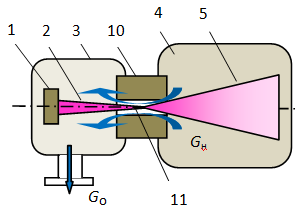
\includegraphics[width=\linewidth]{window_gasdyn.png}\caption{газодинамическое}
  \end{subfigure}
  \caption{Выводные устройства (пособие~[2], рис.~6.2): 1 --- инжектор,
  2 --- пучок, 3 --- высоковакуумная камера, 4 --- рабочая камера, 5 --- ЭПП,
  7 --- фольга, 9 --- шлюзовые камеры, 11 --- газодинамический канал.}
  \label{fig:windows}
\end{figure}

Принцип газодинамического окна: газ из рабочей камеры натекает в
высоковакуумную через канал, а пучок, проходя по каналу, нагревает газ и
стенки. Нагретый газ протекает хуже, и для одномерного течения без
вязкости~[2]
\begin{equation}
    \frac{G_\text{х}}{G_\text{г}} \approx \sqrt{2\,\frac{T_{g\text{г}}}{T_{g\text{х}}} - 1}.
\end{equation}
Нагрев графитовой вставки до $\sim 1000$~К повышает перепад давлений
примерно на порядок по сравнению с холодным каналом. Графит удобен тем,
что \textbf{сублимирует} (нет жидкой фазы, канал не затягивается
расплавом), выдерживает высокий нагрев и химически инертен. В установке
стоят две графитовые вставки по 10~мм с промежуточной откачкой ---
аналог двухступенчатого шлюза.

\subsubsection{Рассеяние электронов в газе}\label{sec:scatter}

Упругое рассеяние на ядрах описывает формула Резерфорда:
\begin{equation}
    \frac{d\sigma}{d\Omega}
    = \left(\frac{Ze^2}{2mv^2}\right)^{\!2}\frac{1}{\sin^4(\theta/2)} .
    \label{eq:ruth}
\end{equation}
Сечение резко растёт при малых углах, поэтому в газе электрон испытывает
\textbf{многократное рассеяние на малые углы}. Средний квадрат угла
растёт линейно с путём, $\langle\theta^2\rangle = N L \int\theta^2 d\sigma$
(с учётом рассеяния на $Z$ электронах атома $\propto Z(Z+1)$), а средний
квадрат радиуса пучка --- как куб пути:
\begin{equation}
    \langle r^2\rangle = \frac{L^3\langle\theta^2\rangle_s}{3} .
\end{equation}
Для \emph{воздуха} и изначально тонкого нерелятивистского пучка~[2, ф.~(2.6)]
\begin{equation}
    r^2\,[\text{см}^2] \approx 400\,\frac{P_m[\text{Торр}]}{T_m[\text{К}]}\,
    \frac{L^3[\text{см}]}{E_b^2[\text{кэВ}]} .
    \label{eq:r2}
\end{equation}
где $T_m$ --- температура газа (у нас комнатная, $T_m \approx 300$~К),
$L$ --- расстояние от точки инжекции. Формула получена для воздуха;
азот по рассеянию почти не отличается от воздуха. Рассеяние растёт с
зарядом ядра ($\langle\theta^2\rangle \propto Z(Z+1)$ на атом): на
молекулу $Z(Z+1) = 2\cdot 7\cdot 8 = 112$ для $\Nt$ и $18\cdot 19 = 342$
для Ar. Поэтому при равном давлении аргон рассеивает пучок примерно в
3 раза сильнее азота.

\paragraph{Где пучок доходит до стенки.} Из~\eqref{eq:r2} пучок
расширяется до радиуса трубки $R$ на расстоянии
\begin{equation}
    z_R \approx \left(\frac{R^2\,T_m E_b^2}{400\,P_m}\right)^{1/3}
    \propto P_m^{-1/3}.
    \label{eq:zR}
\end{equation}
Для внутреннего радиуса $R \approx 1{,}1$~см (внешний 1,24~см минус
стенка) в $\Nt$ получаем $z_R \approx 9{,}4;\ 6{,}9;\ 5{,}5$~см при
$1;\ 2{,}5;\ 5$~Торр. Для Ar множитель $(342/112)^{-1/3} \approx 0{,}69$:
$z_R \approx 6{,}5;\ 4{,}8;\ 3{,}8$~см. Это оценка масштаба, где электроны
массово уходят на стенку; ниже она сравнивается с положением максимума
свечения.

\subsubsection{Торможение электронов. Формула Бете--Блоха}\label{sec:bethe}

В \textbf{модели непрерывного замедления} считают, что энергия теряется
только в неупругих столкновениях, причём непрерывно, и однозначно
определяется пройденным путём. Удельные потери даёт формула
Бете--Блоха (нерелятивистский вид)
\begin{equation}
    -\frac{dE}{dl} = \frac{2\pi N_A e^4 Z\rho}{A\,E}\,
    \ln\frac{bE}{I_\text{ср}}, \qquad b = 1{,}17,
    \label{eq:bethe}
\end{equation}
где $I_\text{ср}$ --- средняя энергия возбуждения атома ($87$~эВ для
$\Nt$, $190$~эВ для Ar).

\paragraph{Применимость формулы Бете--Блоха (вопрос преподавателя).}
\textbf{\emph{Применимость ограничена снизу.}} При малых $E$ формула
неверна по двум причинам~[2, с.~37--40]:
\begin{enumerate}
  \item \emph{$I_\text{ср}$ зависит от энергии:} при энергиях, сравнимых
        с энергиями связи, возбуждаются не все оболочки атома, и
        $I_\text{ср} = I_\text{ср}(E)$ уже не константа;
  \item \emph{логарифм меняет знак:} если $\varepsilon = bE/I_\text{ср} \le 1$,
        то $\ln(bE/I_\text{ср}) \le 0$, и из~\eqref{eq:bethe} следует
        $dE/dl \ge 0$, то есть электрон будто бы набирает энергию, что
        лишено смысла.
\end{enumerate}
\textbf{Нижней границей применимости считают $E \approx 150$~эВ}; на ней
обрывают траектории и в расчёте Монте-Карло. Подробнее --- ответ~3 в
разделе <<Вопросы преподавателя>>.

\paragraph{Оценки для наших условий.}
Формула~\eqref{eq:bethe} даёт
$-dE/dl \approx 12$~эВ/см ($\Nt$) и $13$~эВ/см (Ar) при 1~Торр,
пропорционально давлению. Даже при 5~Торр на длине трубки (31~см)
электрон теряет лишь $\approx 2$~кэВ $\approx 7\%$ энергии.
Экстраполированный пробег в воздухе~[2, ф.~(2.14)]
\begin{equation}
    R_\text{э}\,[\text{м}] \approx 1{,}1\cdot 10^{-4}\,E_b^{1{,}7}\,
    \frac{T_m}{P_m} \approx \frac{10{,}7}{P_m[\text{Торр}]}
    \qquad (E_b = 30~\text{кэВ},\ T_m = 300~\text{К}).
    \label{eq:range}
\end{equation}
На другие газы пересчитываем через массовую толщину: пробег, выраженный
в мг/см$^2$ [2, ф.~(2.13)], от газа почти не зависит, поэтому
$R_\text{э} \propto 1/\rho \propto 1/(P_m M)$:
\begin{equation}
    R_\text{э}^{\Nt} \approx \frac{11{,}1}{P_m}~\text{м}, \qquad
    R_\text{э}^{\text{Ar}} \approx \frac{7{,}8}{P_m}~\text{м}.
\end{equation}
При 1--5~Торр это $1{,}6$--$11$~м, то есть \textbf{много больше длины трубки}.
Профиль свечения в трубке определяется не пробегом, а рассеянием пучка и
уходом электронов на стенки.

\subsubsection{Энерговыделение и свечение ЭПП}
\label{sec:edep}

Основная реакция образования ЭПП --- ионизация электронным ударом:
\begin{equation}
    \mathrm{A} + e_b \to \mathrm{A}^+ + e_p + e_b .
\end{equation}
Первичный электрон ($E_b = 30$~кэВ $\gg I \sim 10$~эВ) рождает в цепочке
столкновений $E_b/U_i \sim 10^3$ вторичных электронов $e_p$, которые и
сами могут ионизовать. Кроме ионов и электронов в ЭПП есть возбуждённые
атомы и молекулы A$^*$; именно они и светятся. При торможении электронов возникает также
тормозное рентгеновское излучение, поэтому установка защищена свинцом.

Функция распределения электронов по энергиям (деградационный спектр)
немаксвелловская (рис.~3.3 пособия~[2]): узкий пик у $E_b$ (источник);
длинный <<хвост>> каскада от $E_b$ до порогов ионизации ($\sim 15$~эВ),
электроны которого ещё ионизуют и возбуждают; <<голова>> из медленных
электронов, возбуждающих колебания и вращения. Это ещё одна причина
неравновесности ЭПП.

\textbf{Скорость ионизации} (число пар в единице объёма в единицу
времени)
\begin{equation}
    Q_\text{ion} = \left(-\frac{dE}{dz}\right)\frac{j_b}{e\,U_i},
    \qquad
    Q_\text{ex} = \left(-\frac{dE}{dz}\right)\frac{j_b}{e\,(U_\text{ex})_i},
    \label{eq:Q}
\end{equation}
где $U_i$ --- энергетическая цена пары ($35{,}3$~эВ для $\Nt$, $25{,}4$~эВ
для Ar~[2, табл.~3.4]).

\textbf{Основная гипотеза работы:} интенсивность свечения элементарного
объёма пропорциональна концентрации возбуждённых частиц, а значит,
$B \propto Q_\text{ex}$. Если газ неподвижен, излучение испускается там же,
где произошло возбуждение. Время жизни излучающих состояний составляет
$\sim 10$--$100$~нс, за это время частица смещается на $\sim 10$~мкм.
Тогда $B(z)$ повторяет $Q(z)$. В потоке газа возбуждённые частицы
сносятся, и соответствие нарушается.

\subsubsection{ЭПП в контейнере. Роль стенок}\label{sec:wall}

В трубке пучок рассеивается и выходит на стенку. Отличия от свободной
плазмы:
\begin{itemize}
  \item электроны, попавшие на стенку, поглощаются или отражаются;
        отражённые снова участвуют в ионизации, поглощённые греют стенку;
  \item нагретая стенка греет пристеночный газ. При постоянном давлении
        плотность $n = P/kT$ у стенки падает, что меняет рассеяние и
        энерговыделение;
  \item кварц под ударами быстрых электронов люминесцирует, и это
        свечение добавляется к свечению плазмы;
  \item заряженные частицы уходят на стенку \textbf{амбиполярной
        диффузией}. Быстрые электроны опережают ионы, возникает
        поляризационное поле, которое тормозит электроны и ускоряет ионы,
        и обе компоненты диффундируют вместе:
        \begin{equation}
            D_a = \frac{D_i\mu_e + D_e\mu_i}{\mu_e+\mu_i}
            \approx D_i\left(1+\frac{T_e}{T_i}\right).
        \end{equation}
        Условие амбиполярности $l_D \ll L$ выполняется уже при
        $n_e \gg 10^4$~см$^{-3}$, то есть в ЭПП всегда. Радиус трубки
        задаёт время диффузионного ухода зарядов $\tau_d \sim R^2/D_a$.
\end{itemize}

\subsubsection{Излучение плазмы и излучение стенок}
\label{sec:quartz}

Камера и спектрометр видят сразу и плазму, и стенку трубки. Стенка может
излучать двумя способами~[2, с.~75--77]:
\begin{itemize}
  \item \textbf{тепловое излучение} нагретой стенки и деталей установки.
        Спектр непрерывный, описывается законами Вина и
        Стефана--Больцмана и лежит в красной и ближней ИК-области. На
        панорамных спектрах оно распознаётся однозначно;
  \item \textbf{катодолюминесценция} (<<холодное свечение>>) кварца под
        ударами быстрых электронов, а также фото- и
        рентгенолюминесценция. Её спектр тоже \emph{непрерывный}.
\end{itemize}
Излучение ЭПП, наоборот, \emph{линейчатое и полосатое} (атомные линии,
молекулярные полосы). Поэтому наблюдаемый спектр --- суперпозиция линий
плазмы и непрерывного фона стенки. На рис.~\ref{fig:quartz}а показан
спектр ЭПП азота у кварцевой пластины: полосы $\Nt$ и $\mathrm{N}_2^+$
стоят на широком горбе люминесценции кварца (400--600~нм, максимум
около 470~нм). У других материалов, например керамики Al$_2$O$_3$
(рис.~\ref{fig:quartz}б), спектр люминесценции отличается и формой, и
диапазоном.

\begin{figure}[H]
  \centering
  \begin{subfigure}{0.48\linewidth}
    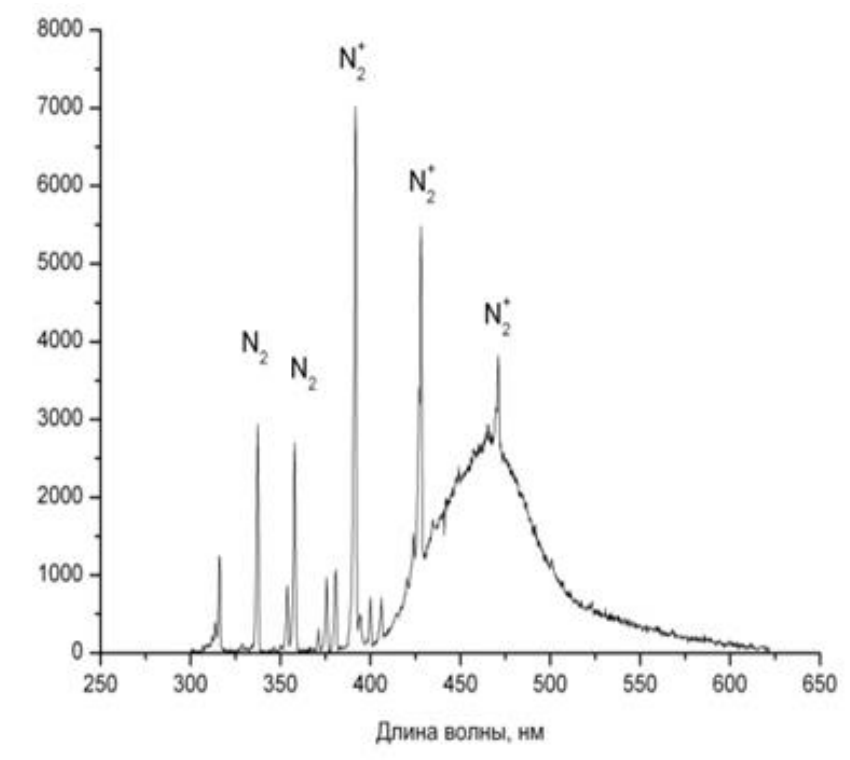
\includegraphics[width=\linewidth]{book_fig4_11_quartz.png}
    \caption{ЭПП азота на фоне люминесценции кварца}
  \end{subfigure}\hfill
  \begin{subfigure}{0.48\linewidth}
    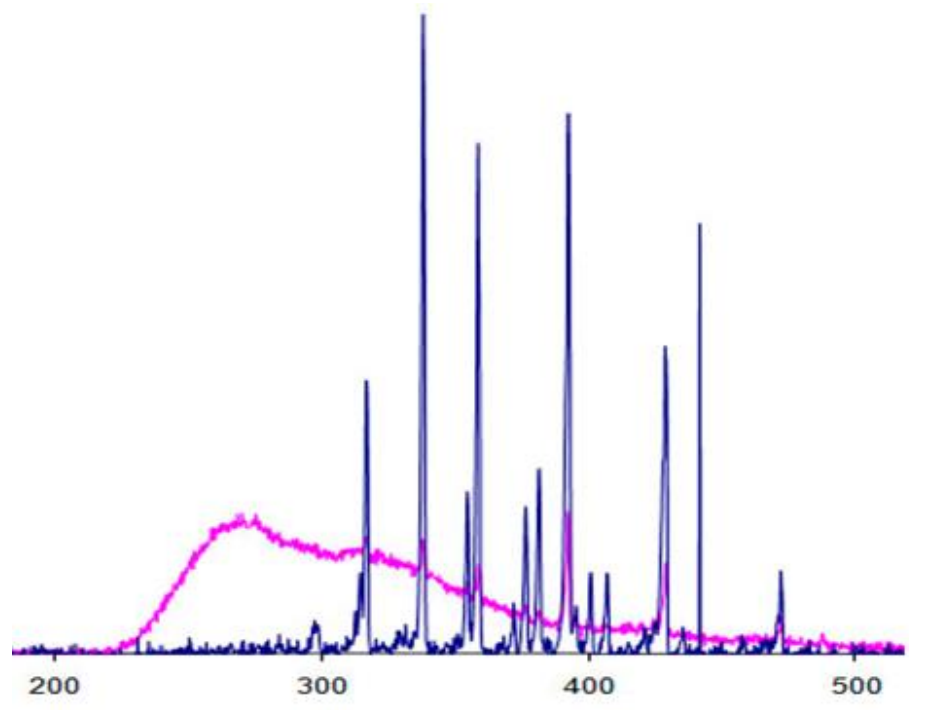
\includegraphics[width=\linewidth]{book_fig4_12_al2o3.png}
    \caption{ЭПП азота (синий) и люминесценция Al$_2$O$_3$ (красный)}
  \end{subfigure}
  \caption{Разделение излучения плазмы и стенки по спектру~[2, рис.~4.11,
  4.12]. По оси абсцисс --- длина волны, нм.}
  \label{fig:quartz}
\end{figure}

Отсюда \textbf{способ отделить излучение плазмы от излучения кварца}:
\begin{enumerate}
  \item \emph{спектральный} (основной): записать панорамный спектр,
        провести под линиями и полосами непрерывную базовую линию
        (континуум кварца) и вычесть её. Интенсивность плазмы --- площадь
        линий над континуумом. Для изображений --- снимать через
        узкополосный фильтр на линии газа вдали от максимума
        люминесценции кварца;
  \item \emph{контрольный опыт}: снять спектр плазмы без стенки/мишени и
        спектр люминесценции материала отдельно и сравнить с суммой
        (как на рис.~\ref{fig:quartz}б);
  \item \emph{инженерный}: уменьшить попадание быстрых электронов на
        стенку --- взять трубку большего диаметра или сжать пучок
        продольным магнитным полем.
\end{enumerate}
Для нашей обработки важно, что горб люминесценции кварца (400--600~нм)
частично попадает в зелёный канал камеры. Поэтому там, где пучок
выходит на стенку (за максимумом $B(z)$), свечение может быть немного
завышено.

\subsubsection{Моделирование методом Монте-Карло}\label{sec:mc}

Программа <<ДОЗА>> прослеживает траектории отдельных электронов
(взаимодействием электронов пучка между собой пренебрегают). Для
каждого электрона:
\begin{enumerate}
  \item разыгрываются точка старта в сечении выводного окна и
        направление с распределением
        $\exp[-(1-\cos\theta)/\theta_0^2]$, $\theta_0$ --- начальная
        угловая расходимость;
  \item длина свободного пробега до упругого столкновения находится из
        $\int_0^s n\,\sigma_{el}\,dr = -\ln\xi$ (сечение Резерфорда с
        экранированием и поправкой Фано), $\xi\in[0,1]$ --- случайное число;
  \item на шагах вдоль траектории потери энергии считаются по
        Бете--Блоху и записываются в ячейки сетки (это и есть $Q(z,r)$);
  \item разыгрывается новый угол рассеяния; процесс повторяется до
        $E < 150$~эВ или выхода из области; отражение от стенки и
        нагрев газа и стенки учитываются самосогласованно.
\end{enumerate}

\subsection{Экспериментальная установка}

\begin{figure}[H]
  \centering
  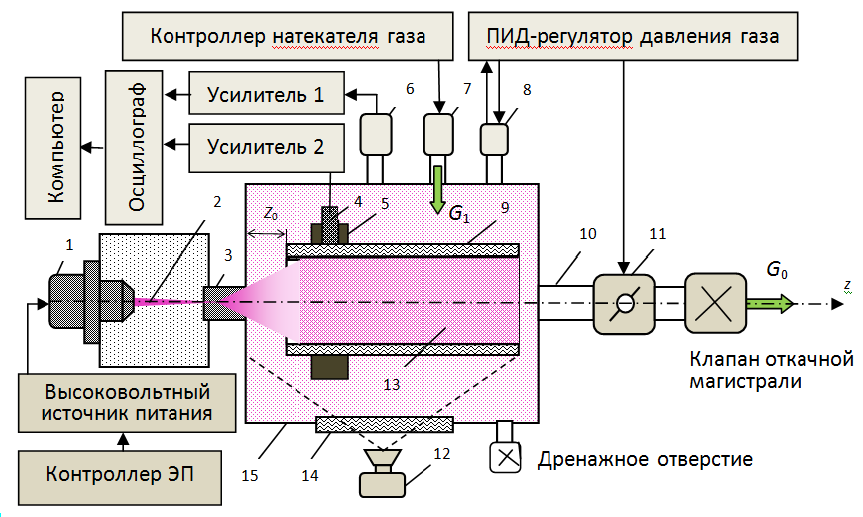
\includegraphics[width=0.85\linewidth]{scheme_epp.png}
  \caption{Схема установки~[1]: 1 --- электронная пушка, 2 --- пучок,
  3 --- выводное газодинамическое окно, 4 --- фотоприёмник,
  6, 8 --- вакуумметры, 7 --- натекатель газа, 9 --- кварцевая трубка,
  10 --- вакуумная магистраль, 11 --- мотыльковый клапан, 12 --- CCD-камера,
  13 --- ЭПП, 14 --- смотровое окно, 15 --- рабочая камера.}
  \label{fig:scheme_epp}
\end{figure}

Тонкий пучок, сформированный пушкой (1) с катодом LaB$_6$ в
высоковакуумной камере, через газодинамическое окно (3) инжектируется в
рабочую камеру (15) с плазмообразующим газом. Кварцевая трубка (9)
(длина $310$~мм, внешний диаметр $24{,}8$~мм) соосна пучку; координата
$z$ отсчитывается от торца трубки со стороны пучка. Трубка крепится
адаптерами, объединёнными с выводным окном (п.~1.3.1 методички), поэтому
считаем зазор $z_0$ между окном и трубкой малым, и $z$ --- это расстояние
от точки инжекции (так же построен рис.~6.8 пособия~[2]). Давление
поддерживает ПИД-регулятор: баратрон MKS~626A, мотыльковый клапан
MKS~253B, натекатель MKS~1179B. Свечение снимается CCD-камерой (12)
через смотровое окно (14).

\subsection{Методика измерений и обработки}\label{sec:method1}

\begin{itemize}
  \item Давление $P_m$ задаётся ПИД-регулятором (1; 2,5; 5~Торр) и
        контролируется баратроном.
  \item Для каждого газа и давления сделан снимок светящейся трубки при
        одинаковых настройках камеры (6 снимков).
  \item Обработка (\texttt{main.py}): загрузка снимка (Pillow), выбор
        \textbf{зелёного канала} (обоснование ниже), вычитание фона
        (медиана тёмной области кадра). Затем $B(z)$ находится усреднением яркости
        по полосе внутри трубки (143 пикселя поперёк оси); полоса $\pm\sigma$
        на графиках --- разброс яркости по этому сечению. Профили
        нормированы на максимум.
  \item \textbf{Калибровка} $z$: дальний торец трубки находится как точка
        самого резкого спада $B(z)$ на снимках при 1~Торр (3122 и
        3106~пикселей), и он соответствует $z = 310$~мм. Получаем
        $0{,}0996$~мм/пиксель. Проверка: видимый диаметр трубки
        $255$~пикселей $= 25{,}4$~мм против паспортных $24{,}8$~мм
        (расхождение 2\%). Далее $z$ --- в сантиметрах, как в расчёте
        Монте-Карло.
  \item Положение максимума $z_\text{max}$ ищется по профилю,
        сглаженному окном 51~пиксель ($\approx 5$~мм). Погрешность
        $\Delta z$ --- полуширина области, где профиль $\ge 0{,}98\,B_\text{max}$
        (пик пологий).
\end{itemize}

\paragraph{Почему достаточно одного (зелёного) канала.}
Цветная камера даёт три канала R, G, B. Для полосы усреднения на
снимках ЭПП:
\begin{center}
  \begin{tabular}{lccc}
    \toprule
    Канал & средний сигнал (из 255) & насыщено пикселей & $z_\text{max}$ по каналу, см \\
    \midrule
    R (красный) & 14--46  & 0       & 0,4--10,5 \\
    G (зелёный) & 48--140 & 0       & 2,4--13,1 \\
    B (синий)   & 96--232 & 3--58\% & 2,2--11,1 \\
    \bottomrule
  \end{tabular}
\end{center}
\begin{itemize}
  \item \textbf{Синий} канал самый яркий (полосы $\Nt$ и $\mathrm{N}_2^+$
        лежат в УФ и фиолетовой области), но насыщен. На насыщенных
        участках профиль срезан, и положение максимума искажается.
  \item \textbf{Красный} канал не насыщен, но сигнал слабый (при 5~Торр
        в Ar всего $\approx 14$ отсчётов), и шум сравним с полезным
        сигналом.
  \item \textbf{Зелёный} канал не насыщен ни на одном снимке и имеет
        достаточный сигнал. Это единственный канал, пригодный для всех
        шести режимов.
\end{itemize}
Использовать только один канал можно, потому что нам нужна
\emph{форма} $B(z)/B_\text{max}$, а не абсолютная яркость. По гипотезе
$B\propto Q$ свечение в любой полосе спектра пропорционально
энерговыделению, если спектральный состав излучения не меняется вдоль
$z$. Это выполняется, потому что возбуждение идёт вторичными электронами
с деградационным спектром, форма которого почти не зависит от $z$
(п.~\ref{sec:edep}). Проверка: максимумы по красному каналу совпадают с
зелёными в пределах погрешности в 5 режимах из 6. Исключение --- Ar при
5~Торр, где красный сигнал почти не отличается от шума.

\subsection{Результаты}

\subsubsection{Первичные данные}

\begin{figure}[H]
  \centering
  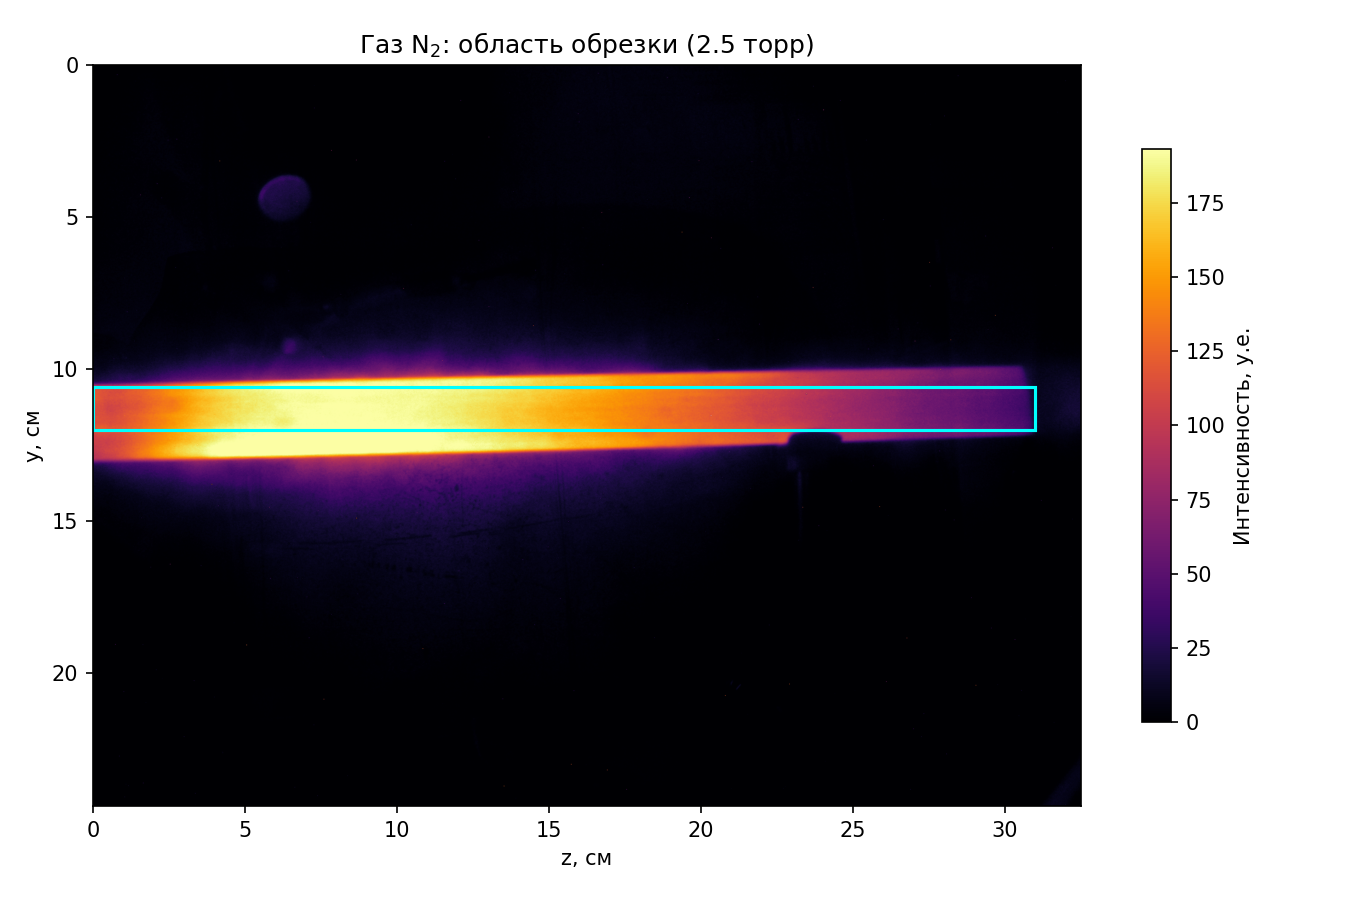
\includegraphics[width=0.75\linewidth]{t1_crop_N2_2.5torr.png}
  \caption{Снимок ЭПП азота при 2,5~Торр (зелёный канал, фон вычтен);
  рамка --- полоса усреднения. Пучок входит слева.}
  \label{fig:t1_crop}
\end{figure}

\begin{figure}[H]
  \centering
  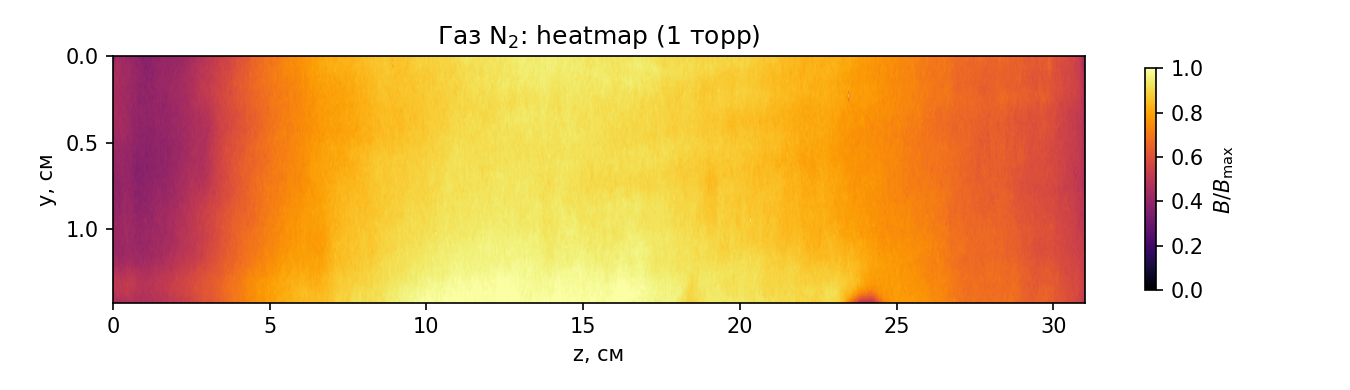
\includegraphics[width=0.49\linewidth]{t1_heatmap_N2_1torr.png}\hfill
  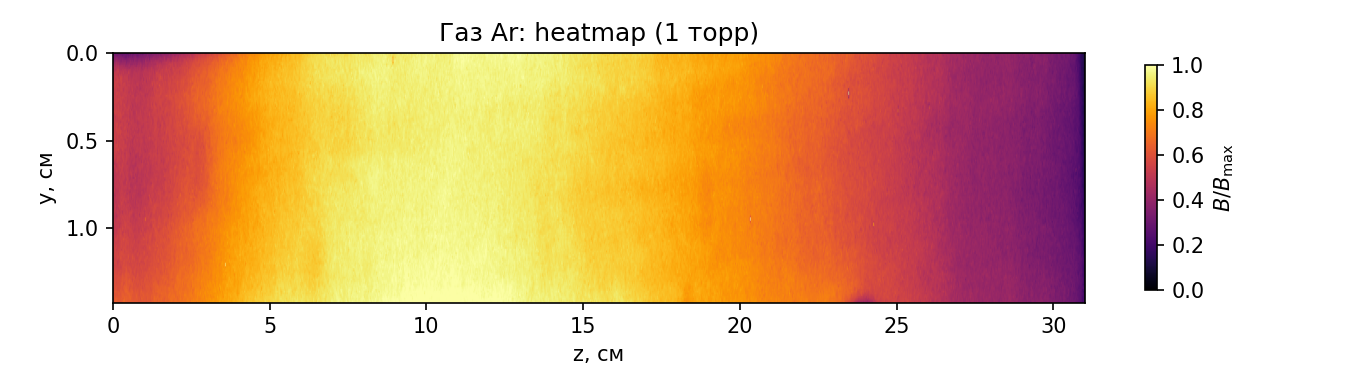
\includegraphics[width=0.49\linewidth]{t1_heatmap_Ar_1torr.png}\\
  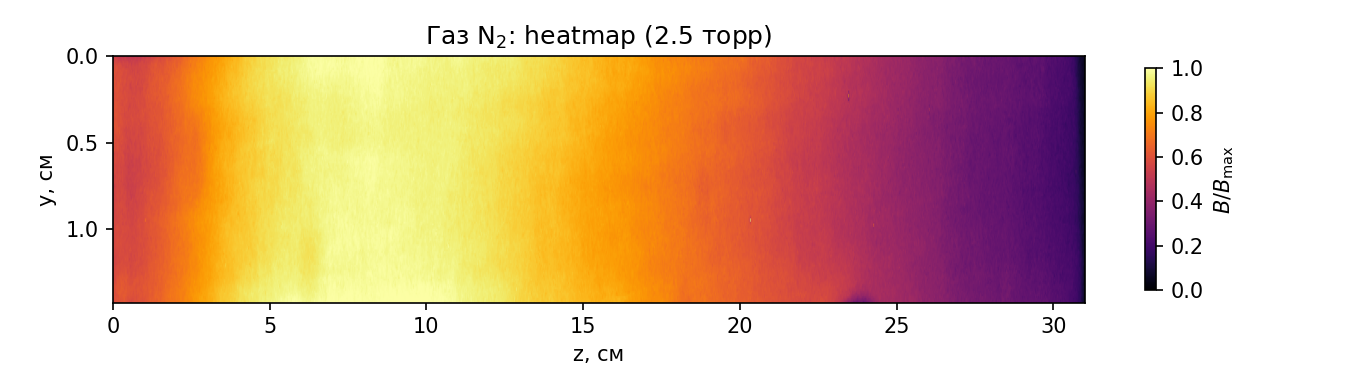
\includegraphics[width=0.49\linewidth]{t1_heatmap_N2_2.5torr.png}\hfill
  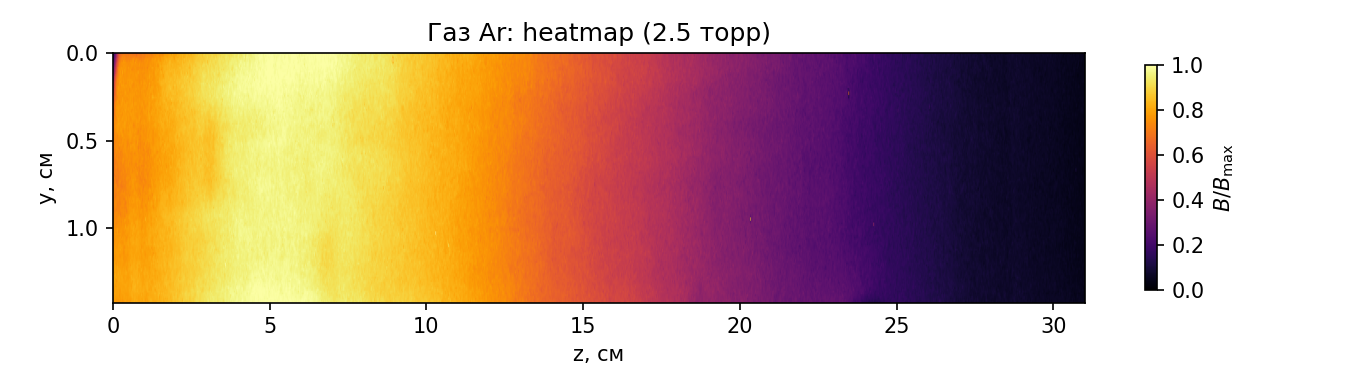
\includegraphics[width=0.49\linewidth]{t1_heatmap_Ar_2.5torr.png}\\
  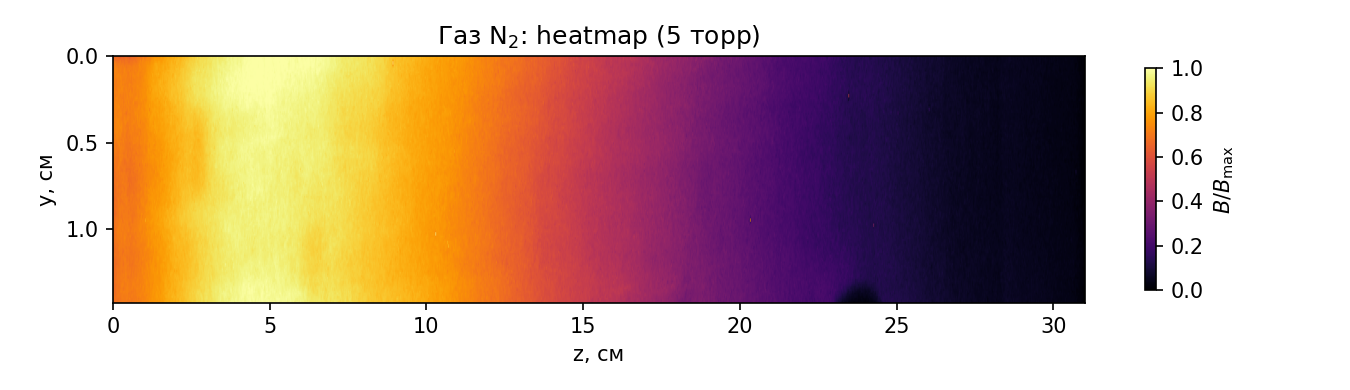
\includegraphics[width=0.49\linewidth]{t1_heatmap_N2_5torr.png}\hfill
  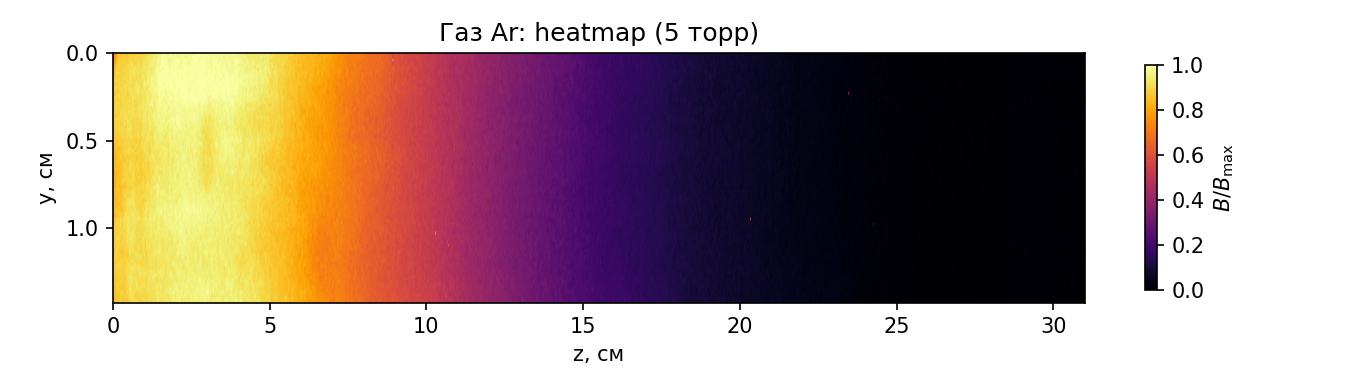
\includegraphics[width=0.49\linewidth]{t1_heatmap_Ar_5torr.png}
  \caption{Карты яркости полосы усреднения: слева $\Nt$, справа Ar;
  сверху вниз 1; 2,5; 5~Торр.}
  \label{fig:t1_heat}
\end{figure}

\subsubsection{Профили $B(z)$}

\begin{figure}[H]
  \centering
  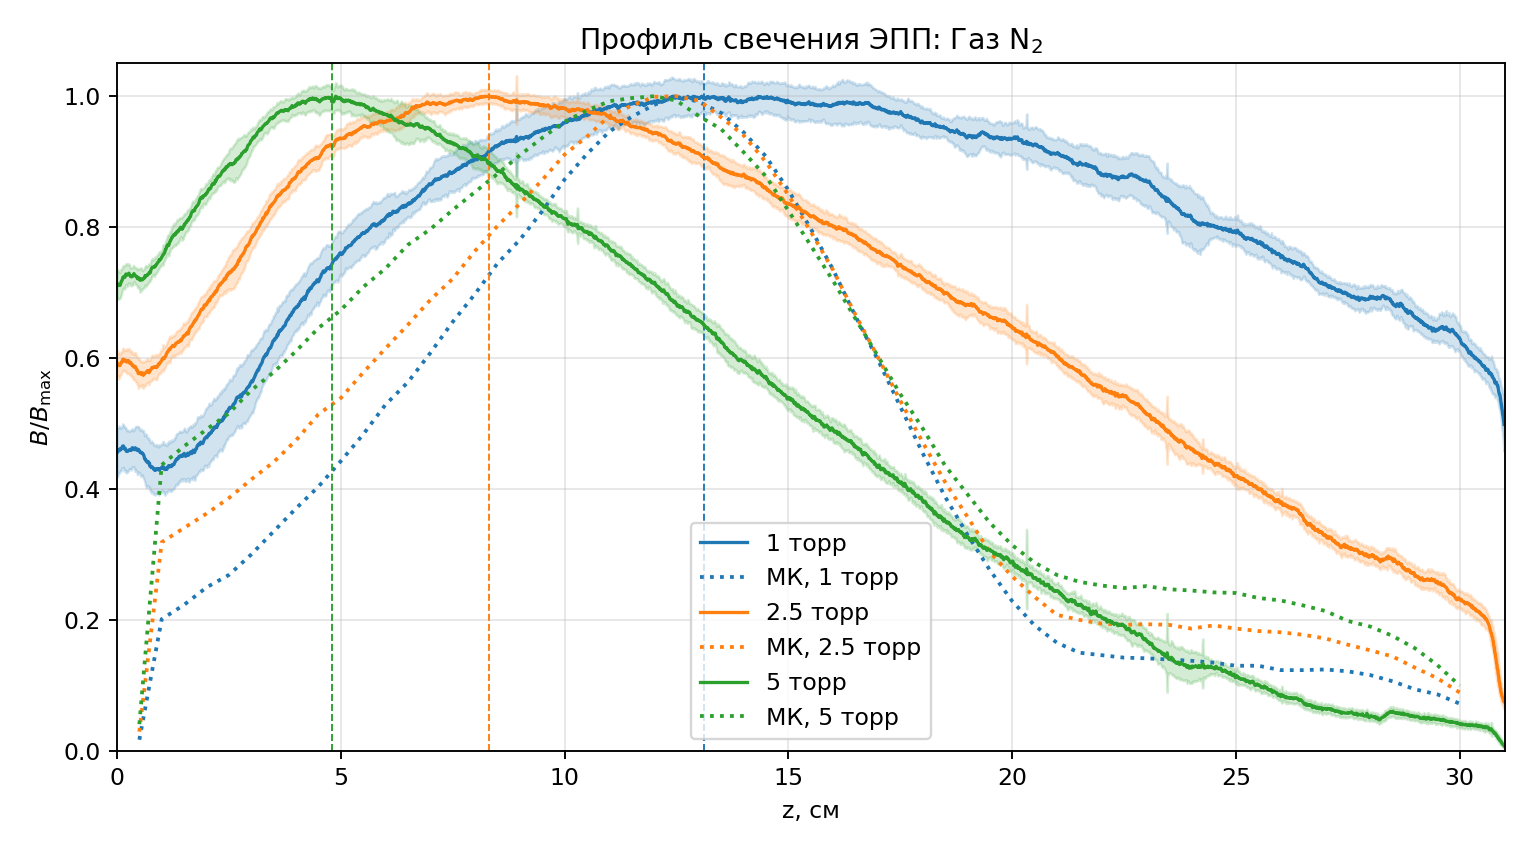
\includegraphics[width=0.85\linewidth]{t1_profile_N2.png}
  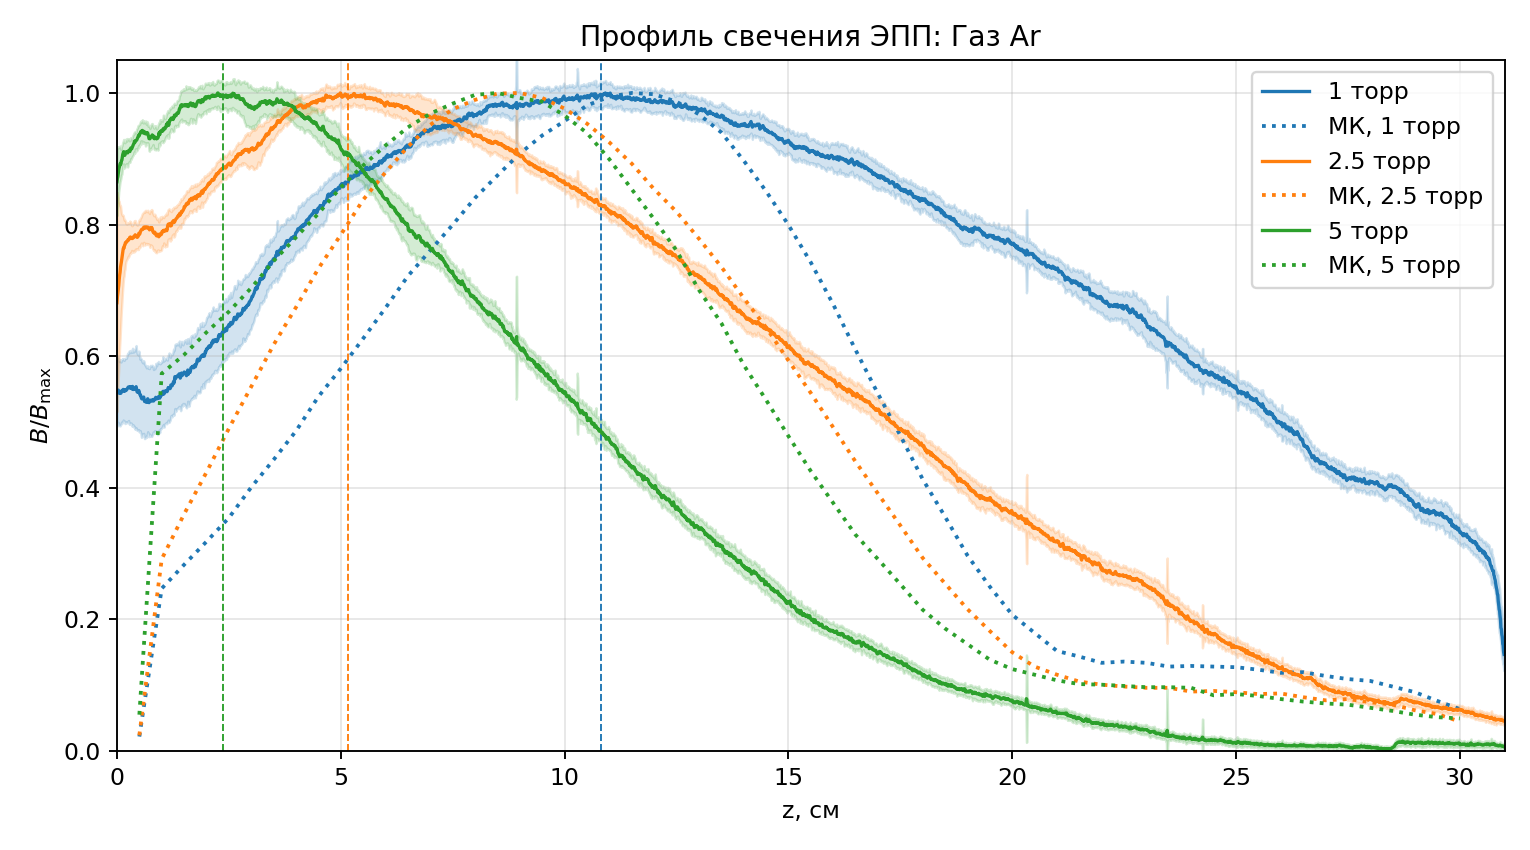
\includegraphics[width=0.85\linewidth]{t1_profile_Ar.png}
  \caption{Продольные профили свечения ЭПП $B(z)/B_\text{max}$ в азоте
  (сверху) и аргоне (снизу), полоса --- $\pm\sigma$ по полоске. Штриховые
  линии --- положения максимумов, пунктир --- расчёт Монте-Карло
  $E(z)/E_\text{max}$ (п.~\ref{sec:mcres}) того же цвета.}
  \label{fig:t1_prof}
\end{figure}

\begin{table}[H]
  \centering
  \caption{Положение максимума свечения $z_\text{max}$, относительная
  яркость у окна $B(0)/B_\text{max}$ и экстраполированный пробег
  $R_\text{э}$ (ф.~\eqref{eq:range} с пересчётом на газ по массовой
  толщине, $E_b = 30$~кэВ, $T_m = 300$~К).}
  \label{tab:t1}
  \begin{tabular}{ccccc}
    \toprule
    Газ & $P_m$, Торр & $z_\text{max}$, см & $B(0)/B_\text{max}$ &
    $R_\text{э}$, м \\
    \midrule
    $\Nt$ & 1   & $13{,}1 \pm 3{,}2$ & 0,46 & 11,1 \\
    $\Nt$ & 2,5 & $8{,}3 \pm 1{,}9$  & 0,59 & 4,4 \\
    $\Nt$ & 5   & $4{,}8 \pm 1{,}1$  & 0,71 & 2,2 \\
    \midrule
    Ar & 1   & $10{,}8 \pm 2{,}3$ & 0,55 & 7,8 \\
    Ar & 2,5 & $5{,}2 \pm 1{,}2$  & 0,68 & 3,1 \\
    Ar & 5   & $2{,}4 \pm 1{,}2$  & 0,87 & 1,6 \\
    \bottomrule
  \end{tabular}
\end{table}

\begin{figure}[H]
  \centering
  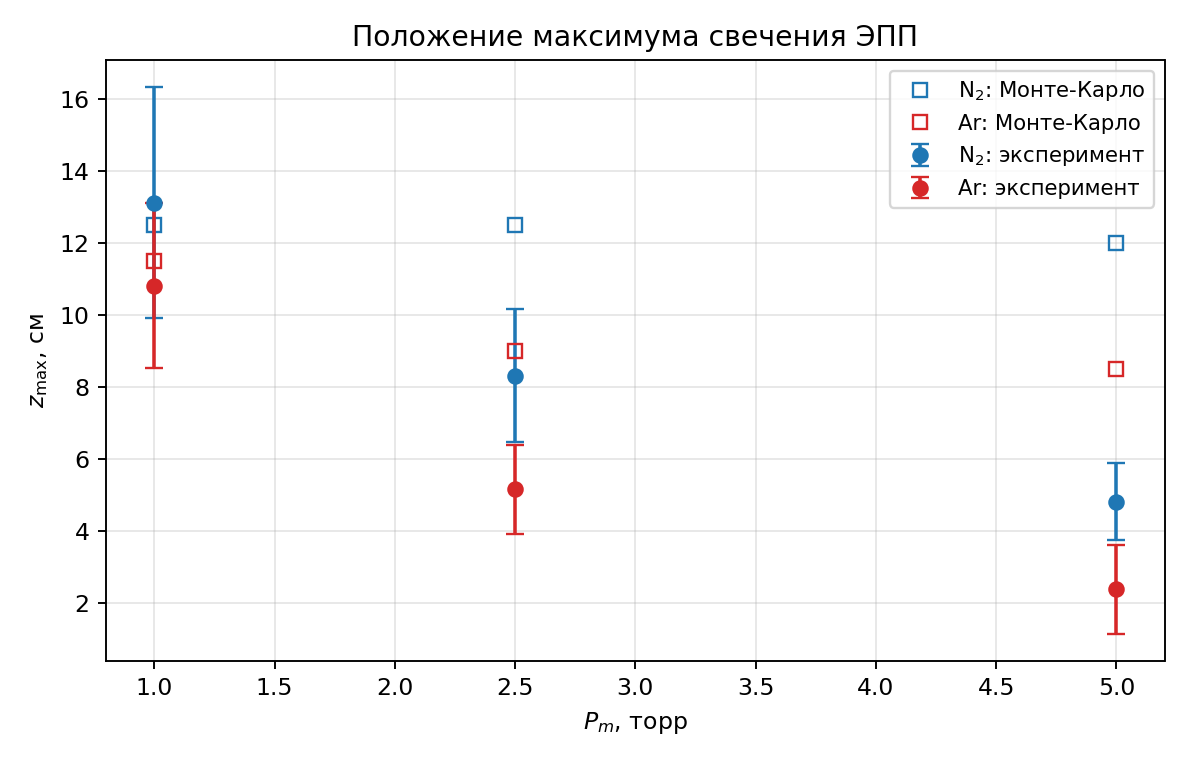
\includegraphics[width=0.7\linewidth]{t1_zmax.png}
  \caption{Положение максимума свечения от давления: эксперимент
  (точки с погрешностями) и расчёт Монте-Карло (пустые квадраты).}
  \label{fig:zmax}
\end{figure}

\subsubsection{Вычислительный эксперимент}\label{sec:mcres}

Расчёт выполнен для тех же шести режимов, что и опыт (газ, давление,
геометрия трубки), табл.~\ref{tab:mc}. Угол раствора пучка
$\theta_0 = 3{,}5^\circ$ во всех расчётах, кроме Ar при 2,5~Торр, где
$\theta_0 = 7^\circ$.

\begin{table}[H]
  \centering
  \caption{Параметры расчётов методом Монте-Карло.}
  \label{tab:mc}
  \begin{tabular}{lccc}
    \toprule
    Газ & $P_m$, Торр & $\theta_0$ & $z_\text{max}^\text{МК}$, см \\
    \midrule
    $\Nt$ & 1   & $3{,}5^\circ$ & $12{,}5\pm0{,}25$ \\
    $\Nt$ & 2,5 & $3{,}5^\circ$ & $12{,}5\pm0{,}25$ \\
    $\Nt$ & 5   & $3{,}5^\circ$ & $12{,}0\pm0{,}25$ \\
    Ar    & 1   & $3{,}5^\circ$ & $11{,}5\pm0{,}25$ \\
    Ar    & 2,5 & $7^\circ$     & $9{,}0\pm0{,}25$ \\
    Ar    & 5   & $3{,}5^\circ$ & $8{,}5\pm0{,}25$ \\
    \bottomrule
  \end{tabular}
\end{table}

Методичка (п.~1.5) предлагает сначала подобрать на одном режиме число
траекторий (2000--7000) и угол $\theta_0$ (1--10$^\circ$) по наилучшему
согласию с опытом, а затем считать все режимы с этим набором. Мы
приняли $\theta_0 = 3{,}5^\circ$ для всех режимов. Для Ar при 2,5~Торр
есть только расчёт с $\theta_0 = 7^\circ$, поэтому эту точку мы не
используем при обсуждении зависимости от давления: смена угла сама
сдвигает максимум.

Программа выдаёт гистограмму энерговыделения $E(z)$ с шагом 0,5~см на
длине 0,5--30~см. Графики получены в виде изображений и оцифрованы
скриптом \texttt{digitize\_mc.py}. Ось $E$ калибровалась по линиям
сетки, высота каждого столбца бралась по его собственному цвету, чтобы
линия, проведённая поверх столбцов, не искажала значение. Погрешность
оцифровки $\approx 1$~у.е. по $E$ и $\pm 0{,}25$~см по $z$ (полуширина
бина). Результаты, нормированные на максимум, показаны на рис.~\ref{fig:mc}.

\begin{figure}[H]
  \centering
  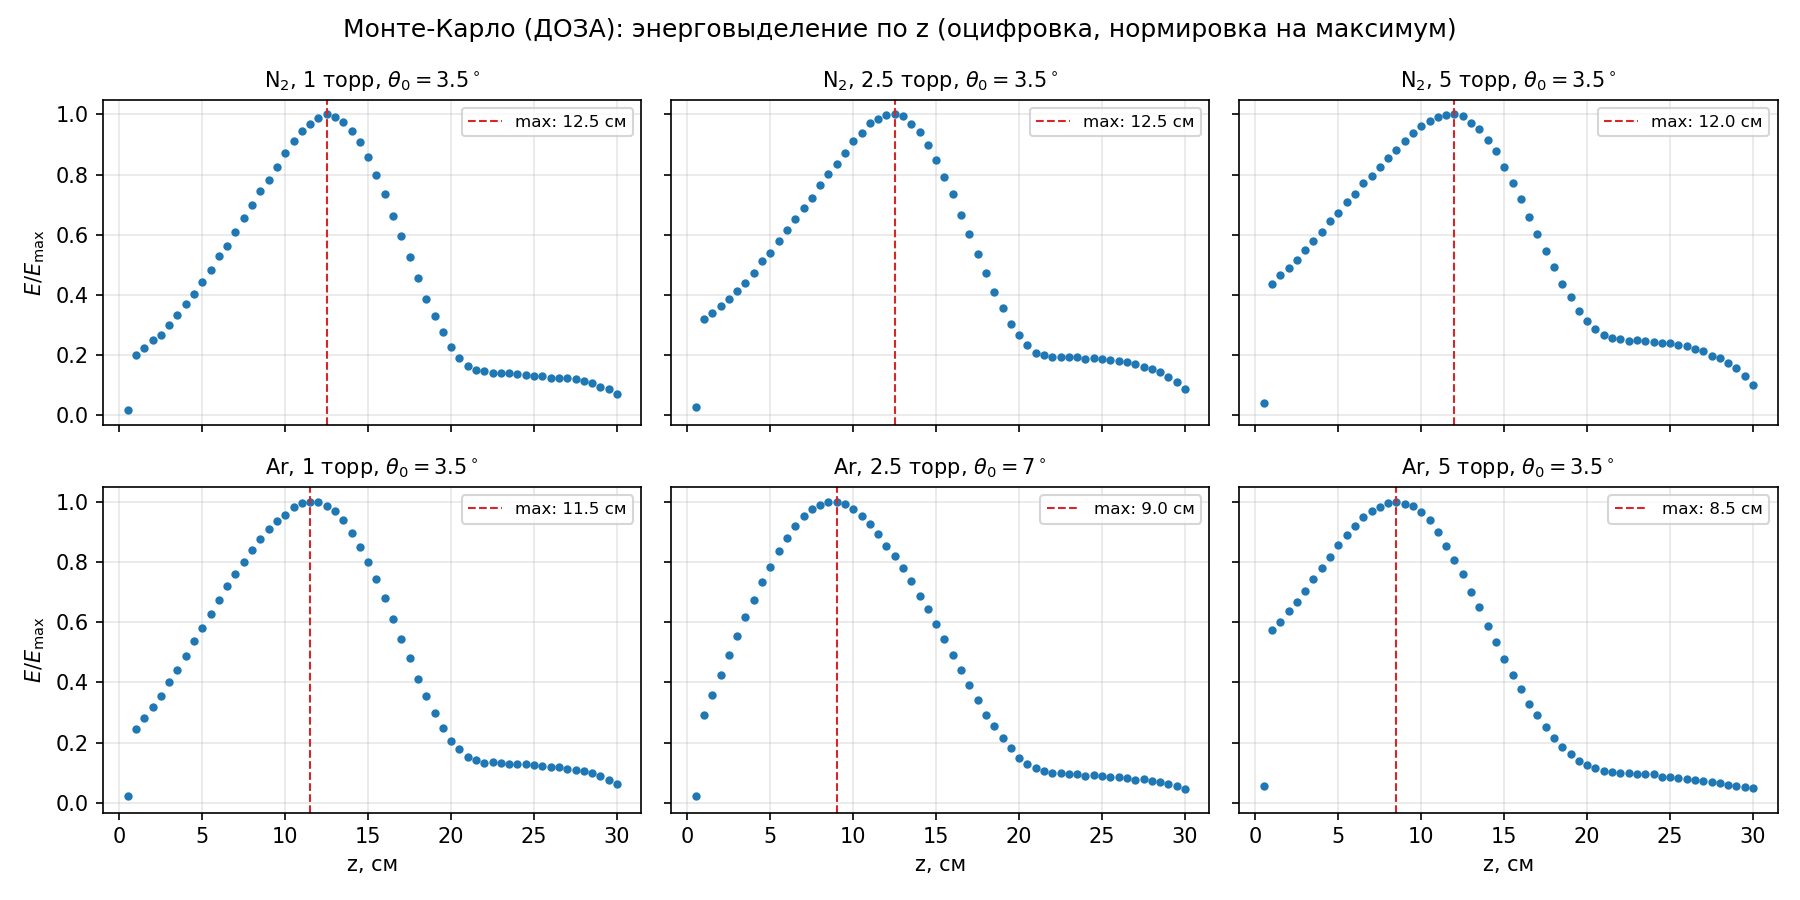
\includegraphics[width=\linewidth]{mc_digitized.png}
  \caption{Энерговыделение $E(z)/E_\text{max}$ по расчётам методом
  Монте-Карло (ДОЗА), оцифровка: сверху $\Nt$, снизу Ar, слева направо
  1; 2,5; 5~Торр. Штрих --- положение максимума.}
  \label{fig:mc}
\end{figure}

Во всех расчётах максимум лежит при $z = 8{,}5$--$12{,}5$~см. За
максимумом $E(z)$ спадает и при $z\gtrsim 20$~см выходит на пологий
участок $0{,}1$--$0{,}25\,E_\text{max}$.

Странно ведёт себя абсолютная величина расчётного энерговыделения.
Удельные потери пропорциональны плотности газа, поэтому при том же
числе траекторий энерговыделение в трубке при 5~Торр должно быть в
несколько раз больше, чем при 1~Торр (пробег $R_\text{э}\gg$ длины
трубки, пучок не останавливается). В расчёте же площадь под $E(z)$
растёт лишь в 1,5 раза для $\Nt$ (5940 $\to$ 8660~у.е.) и почти не
меняется для Ar (7490 $\to$ 7960~у.е.), а максимум в $\Nt$ почти не
сдвигается. Это указывает на то, что давление в расчёте могло
учитываться не так, как мы предполагаем (или число траекторий
различалось). В заголовках исходных графиков
программа печатает ещё одно значение <<z max>> (например, 14,32~см для
$\Nt$ при 1~Торр), которое не совпадает с положением столбца-максимума.
Мы используем положение максимума гистограммы.

\subsection{Обсуждение}

\begin{enumerate}
  \item \textbf{Форма профиля.} При всех давлениях $B(z)$ имеет максимум
        внутри трубки. Пробег $R_\text{э} = 1{,}6$--$11$~м много больше
        трубки, а потери энергии на её длине $\lesssim 7\%$. Значит,
        максимум не связан с торможением: по Бете--Блоху удельные потери
        вдоль траектории монотонно растут. Как отмечено в
        пособии~[2, с.~43--44], наличие максимума энерговыделения на
        некотором расстоянии от точки инжекции обусловлено
        \emph{угловым рассеянием} электронов. У окна пучок узкий и
        направленный. По мере рассеяния растут длина пути электронов на
        единицу $z$ и число актов ионизации в сечении. Дальше часть
        электронов уходит на стенку и рассеивается назад, ток вперёд
        уменьшается, и $B(z)$ спадает.
  \item \textbf{Сдвиг максимума.} С ростом давления максимум смещается
        \textbf{к выводному окну}: $\Nt$ --- $13{,}1 \to 8{,}3 \to 4{,}8$~см,
        Ar --- $10{,}8 \to 5{,}2 \to 2{,}4$~см при $1 \to 2{,}5 \to 5$~Торр.
        Чем плотнее газ, тем быстрее расширяется пучок
        ($r^2 \propto P_m z^3$, ф.~\eqref{eq:r2}), тем раньше электроны
        доходят до стенки и тем ближе к окну максимум. Одновременно растёт
        $B(0)/B_\text{max}$: при 5~Торр свечение у окна почти максимально.
  \item \textbf{Количественная оценка.} Расстояние $z_R$, на котором
        пучок по~\eqref{eq:zR} расширяется до стенки, в $\Nt$ равно
        $9{,}4;\ 6{,}9;\ 5{,}5$~см, а измеренный $z_\text{max}$ ---
        $13{,}1;\ 8{,}3;\ 4{,}8$~см. Порядок величины и направление сдвига
        совпадают, хотя оценка грубая (формула для воздуха, без
        отражения от стенки, и максимум не обязан приходиться точно на
        $z_R$). Зависимость от давления в опыте сильнее: степенная
        аппроксимация трёх точек даёт $z_\text{max}\propto P_m^{-0{,}62}$
        ($\Nt$) и $P_m^{-0{,}94}$ (Ar) против $P_m^{-1/3}$ в оценке.
        Возможная причина --- нагрев газа и стенки, растущий с
        давлением, и вклад отражённых от стенки электронов, которых
        оценка не учитывает.
  \item \textbf{Род газа.} В аргоне максимум ближе к окну, чем в азоте,
        при всех давлениях: $z_\text{max}^\text{Ar}/z_\text{max}^{\Nt}
        = 0{,}82;\ 0{,}62;\ 0{,}50$. Причина --- более сильное рассеяние на
        тяжёлых ядрах (п.~\ref{sec:scatter}: $Z(Z+1)$ на молекулу 342
        против 112). Оценка~\eqref{eq:zR} даёт для этого отношения
        $(342/112)^{-1/3} \approx 0{,}69$, в середине измеренного
        диапазона.
  \item \textbf{Сравнение с расчётом Монте-Карло.} Это основная проверка
        работы. Нормированный расчёт $E(z)/E_\text{max}$ наложен на профили
        $B(z)/B_\text{max}$ (рис.~\ref{fig:t1_prof}, пунктир), положения
        максимумов --- в табл.~\ref{tab:mc_cmp} и на рис.~\ref{fig:zmax}.

        \begin{table}[H]
          \centering
          \caption{Положение максимума: эксперимент и Монте-Карло.}
          \label{tab:mc_cmp}
          \begin{tabular}{lccc}
            \toprule
            Газ & $P_m$, Торр & $z_\text{max}^\text{эксп}$, см &
            $z_\text{max}^\text{МК}$, см \\
            \midrule
            $\Nt$ & 1   & $13{,}1\pm3{,}2$ & $12{,}5$ \\
            $\Nt$ & 2,5 & $8{,}3\pm1{,}9$  & $12{,}5$ \\
            $\Nt$ & 5   & $4{,}8\pm1{,}1$  & $12{,}0$ \\
            Ar    & 1   & $10{,}8\pm2{,}3$ & $11{,}5$ \\
            Ar    & 2,5 & $5{,}2\pm1{,}2$  & $9{,}0$\,$^{*}$ \\
            Ar    & 5   & $2{,}4\pm1{,}2$  & $8{,}5$ \\
            \bottomrule
          \end{tabular}

          \smallskip
          {\footnotesize $^{*}$ расчёт с $\theta_0 = 7^\circ$, остальные
          --- с $3{,}5^\circ$.}
        \end{table}

        Что совпадает:
        \begin{itemize}
          \item при 1~Торр расчёт и опыт согласуются в пределах погрешности
                для обоих газов (12,5 против $13{,}1\pm3{,}2$~см в $\Nt$,
                11,5 против $10{,}8\pm2{,}3$~см в Ar);
          \item в расчёте, как и в опыте, максимум в аргоне ближе к окну,
                чем в азоте, и в аргоне сдвигается к окну с ростом
                давления ($11{,}5\to 8{,}5$~см при 1 и 5~Торр; точку
                2,5~Торр с другим $\theta_0$ не сравниваем).
        \end{itemize}
        Что не совпадает:
        \begin{itemize}
          \item в расчёте максимум сдвигается с давлением гораздо слабее:
                в $\Nt$ он почти стоит на месте ($12{,}5\to12{,}0$~см), а в
                опыте уходит с 13,1 до 4,8~см. При 2,5 и 5~Торр расхождение
                в 2--4 раза больше погрешности;
          \item за максимумом расчётный $E(z)$ спадает до
                $0{,}1$--$0{,}25$ к $z\approx 20$~см, а измеренное свечение
                при 1--2,5~Торр спадает гораздо медленнее;
          \item у окна расчёт даёт меньше, чем опыт: при $z = 1$~см
                $E/E_\text{max} = 0{,}2$--$0{,}57$, а в опыте
                $B(0)/B_\text{max} = 0{,}46$--$0{,}87$. В первом бине
                (0,5~см) расчётное энерговыделение почти нулевое.
        \end{itemize}
        Возможные причины (подробнее --- ответ~6 в разделе <<Вопросы
        преподавателя>>): (1) свечение газа не обязано повторять
        энерговыделение $B\propto Q$; (2) в зелёный канал попадает
        люминесценция кварца (п.~\ref{sec:quartz}), которая затягивает спад
        за максимумом; (3) параметры пучка в расчёте (угол раствора,
        диаметр, положение трубки) известны неточно, а один и тот же
        $\theta_0$ при всех давлениях может не соответствовать опыту;
        (4) слабая зависимость расчётного максимума от давления вместе
        с почти постоянной площадью под $E(z)$ (п.~\ref{sec:mcres})
        говорит о том, что давление в расчёте, вероятно, задано не так,
        как в опыте; без этого сравнение при 2,5 и 5~Торр нельзя
        считать проверкой модели.
  \item \textbf{Сравнение с литературой.} В пособии~[2, рис.~6.8] для
        аргона в трубке $\varnothing 20$~мм максимумы находятся при
        $\approx 8{,}5;\ 4{,}0;\ 1{,}5$~см, а свечение у начала трубки при
        1~Торр $\approx 0{,}45\,B_\text{max}$. Тенденция и уровень свечения
        у окна те же (у нас $B(0)/B_\text{max} = 0{,}55$ для Ar при 1~Торр).
        Наши пики систематически дальше ($10{,}8;\ 5{,}2;\ 2{,}4$~см).
        Частично это объясняется диаметром трубки: по~\eqref{eq:zR}
        $z_R \propto R^{2/3}$, но разница в диаметре даёт лишь
        10--15\%. Остальное может быть связано с другими энергией и
        расходимостью пучка и зазором $z_0$, которые для рис.~6.8 не
        указаны.
  \item \textbf{Гипотеза о $P_m^*$.} Методичка (п.~1.2.1) предполагает,
        что в каждом сечении есть давление $P_m^*$ с максимальной яркостью
        и что $P_m^*$ зависит от $z$. Для проверки нужны зависимости
        $B(P_m)$ в фиксированных сечениях при многих давлениях (как на
        рис.~6.7 пособия~[2]); у нас только три давления и нормированные
        профили, поэтому эту гипотезу мы не проверяли.
\end{enumerate}

% ===============================================================
\section{Часть 2. Высокочастотный ёмкостный разряд}
% ===============================================================

\subsection{Теоретические сведения}

\subsubsection{ВЧ- и ВЧЕ-разряд}

\textbf{ВЧ-разряд} --- газовый разряд в высокочастотном поле
($f = 10^5$--$10^8$~Гц; стандартная частота $13{,}56$~МГц).
\textbf{Ёмкостный} (ВЧЕ) разряд возбуждается напряжением на электродах,
то есть электрическим полем, в отличие от индукционного, который
возбуждается вихревым полем катушки. В работе используются внутренние
плоскопараллельные электроды, $P_m < 100$~Торр. Степень ионизации
$10^{-8}$--$10^{-7}$, плазма неравновесна.

Энергия передаётся плазме через электроны. При $P_m \sim 10$~Торр частота
столкновений в $\sim 10^3$ раз выше частоты поля, и электроны совершают
дрейфовые колебания с амплитудой $A \approx 1$~мм, много меньше
межэлектродного зазора. Ионы практически неподвижны (их амплитуда
в $\sim 10^2$ раз меньше). У электродов электронный газ периодически
<<отступает>> и обнажает положительный заряд: так формируются
\textbf{приэлектродные слои пространственного заряда} (sheath) толщиной
$\sim A$ с сильным полем. В основном объёме плазма квазинейтральна
(дебаевский радиус $\lesssim 0{,}05$~см). Электроны набирают энергию в
поле (омический нагрев в объёме и <<стохастический>> нагрев колеблющимися
границами слоёв) и ионизуют газ.

\subsubsection{$\alpha$- и $\gamma$-формы}\label{sec:rfforms}

\begin{table}[H]
  \centering
  \caption{Сравнение форм ВЧЕ-разряда~[1]}
  \begin{tabular}{p{0.45\linewidth}p{0.45\linewidth}}
    \toprule
    $\alpha$-форма (слаботочная) & $\gamma$-форма (сильноточная) \\
    \midrule
    низкое давление, низкое напряжение &
    возникает при росте напряжения или давления \\
    поддерживается объёмной ионизацией электронами, нагретыми ВЧ-полем
    в плазме и на колеблющихся границах слоёв &
    главную роль играет вторичная электронная эмиссия из электродов под
    ионной бомбардировкой; вторичные электроны ускоряются в слоях и
    дают лавину \\
    малые плотности тока и $n_e$; ток в слоях --- ток смещения &
    скачок плотности тока ($\times 10$ и больше), заметный нагрев газа;
    ток замыкается током проводимости \\
    свечение слабое и однородное, ярче у электродов; тёмные тонкие слои
    у электродов &
    очень яркие тонкие приэлектродные слои; яркая центральная зона,
    отделённая тёмными слоями (аналог фарадеева тёмного пространства) \\
    \bottomrule
  \end{tabular}
\end{table}

Приэлектродные слои $\gamma$-разряда устроены как катодные слои
тлеющего разряда. Поэтому распределение свечения повторяет
последовательность катодный слой $\to$ отрицательное свечение
$\to$ тёмное пространство $\to$ положительный столб (рис.~\ref{fig:rf_theory}а).
Переход $\alpha \to \gamma$ происходит при критической плотности тока,
которая зависит от давления, частоты, материала электродов и газа.
$\alpha$-разряд существует лишь при $P_m L$ ниже критической величины
(рис.~\ref{fig:rf_theory}б): $\approx 40$~Торр$\cdot$см для воздуха и
$\approx 160$~Торр$\cdot$см для гелия.

\begin{figure}[H]
  \centering
  \begin{subfigure}{0.48\linewidth}\centering
    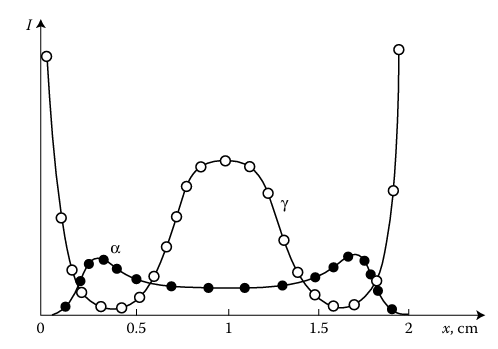
\includegraphics[width=\linewidth]{rf_profile_alpha_gamma.png}
    \caption{$I(x)$ в $\alpha$- и $\gamma$-режимах (воздух, 10~Торр, $L=2$~см)}
  \end{subfigure}\hfill
  \begin{subfigure}{0.42\linewidth}\centering
    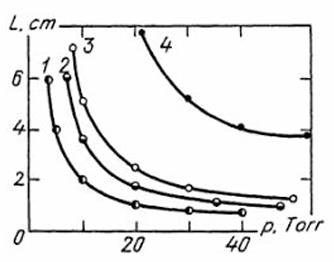
\includegraphics[width=\linewidth]{rf_alpha_boundary.png}
    \caption{границы $\alpha$-разряда: 1 --- $\Nt$, 2 --- воздух,
    3 --- CO$_2$, 4 --- He}
  \end{subfigure}
  \caption{Иллюстрации из методического пособия~[1] (рис.~5 и 6).}
  \label{fig:rf_theory}
\end{figure}

\subsubsection{Оптическое излучение. Оптически тонкая плазма}

Электроны разряда возбуждают атомы гелия, и те светятся своими
линиями. Если в газе есть примесь (азот, пары воды), возбуждённый атом
гелия при столкновении может отдать свою энергию молекуле примеси, и
тогда светится уже она --- своими полосами. Чем больше в объёме молекул
примеси, тем быстрее это происходит. Характерное время передачи
\begin{equation}
    \tau_\text{пер} = \frac{1}{k\,N_\mathrm{A}} ,
    \label{eq:tau4}
\end{equation}
где $N_\mathrm{A}$ --- концентрация примеси, $k$ --- константа скорости
передачи. Если $\tau_\text{пер}$ меньше времени, за которое атом гелия
успевает высветиться сам ($\tau \sim 1$~мкс), то энергия уходит к
примеси, и её полосы становятся ярче линий гелия. При постоянной доле
примеси $N_\mathrm{A}$ растёт с давлением, поэтому есть давление $P^*$,
выше которого в спектре преобладает примесь.

Плазма \textbf{оптически тонкая}, если её оптическая толщина
$\tau_\lambda = \int\kappa_\lambda\,dl \ll 1$: излучение выходит без
поглощения и рассеяния. Тогда регистрируемая интенсивность
пропорциональна интегралу излучательной способности вдоль луча
зрения, и спектры можно сравнивать напрямую.

\subsection{Экспериментальная установка}

\begin{figure}[H]
  \centering
  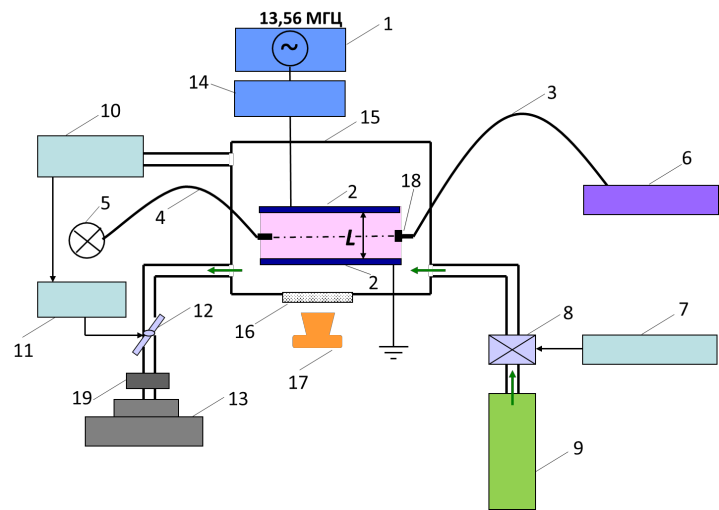
\includegraphics[width=0.8\linewidth]{scheme_rf.png}
  \caption{Схема установки ВЧЕ-разряда~[1]: 1 --- ВЧ-генератор
  Genesis GHW-12 (13,56~МГц), 2 --- плоскопараллельные электроды,
  3, 4 --- световоды, 5 --- эталонный источник света, 6 --- спектрометр
  AvaSpec-2048-2, 7, 8 --- натекатель с контроллером, 10 --- вакуумметр,
  11 --- ПИД-регулятор, 12 --- мотыльковый клапан, 14 --- согласующее
  устройство, 15 --- газоразрядная камера, 17 --- CCD-камера.}
  \label{fig:scheme_rf}
\end{figure}

Межэлектродный зазор $L = 37{,}0$--$37{,}4$~мм, далее
$L = 37{,}2 \pm 0{,}2$~мм. Мощность генератора 30--50~Вт. Газы: гелий
высокой чистоты и технический гелий (с примесью воздуха); давления
1; 2,5; 5~Торр (технический гелий --- также 10~Торр). Камера: диафрагма
$f/3{,}6$, выдержка $1/4$~с. Время съёмки: чистый He --- 10:33, 10:35,
10:37; технический --- $\approx$10:42, 10:45, 10:46, 10:48.

\subsection{Методика обработки}

Профиль $I(L)$ находится усреднением яркости (зелёный канал, фон
вычтен) по полоске шириной 200~пикселей поперёк оси $L$, выбранной слева
от стойки держателя. По $L$ полоска идёт от края верхнего электрода
(945~пиксель) до края нижнего (1620~пиксель). Края электродов определены
по резкому спаду яркости. Масштаб: $675$~пикселей $= 37{,}2$~мм,
$0{,}055$~мм/пиксель. Координата $L$ отсчитывается от верхнего электрода.
Для технического гелия те же профили построены также по красному
каналу, где лежат полосы азота (п.~\ref{sec:red}).

\subsection{Результаты}

\begin{figure}[H]
  \centering
  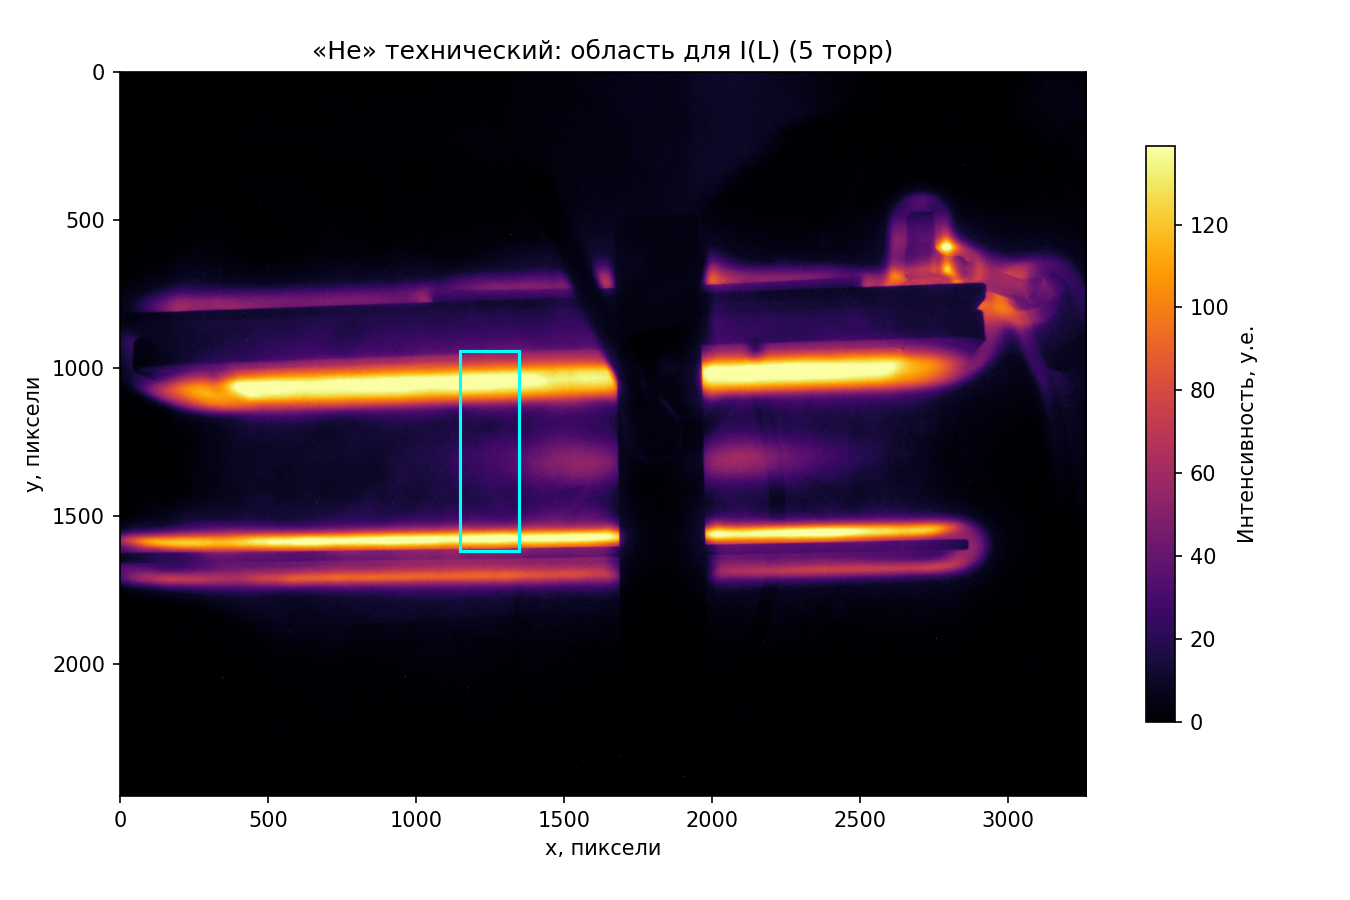
\includegraphics[width=0.7\linewidth]{t2_crop_He_tech_5torr.png}
  \caption{Снимок ВЧЕ-разряда в техническом гелии при 5~Торр;
  рамка --- полоска для $I(L)$.}
  \label{fig:t2_crop}
\end{figure}

\begin{figure}[H]
  \centering
  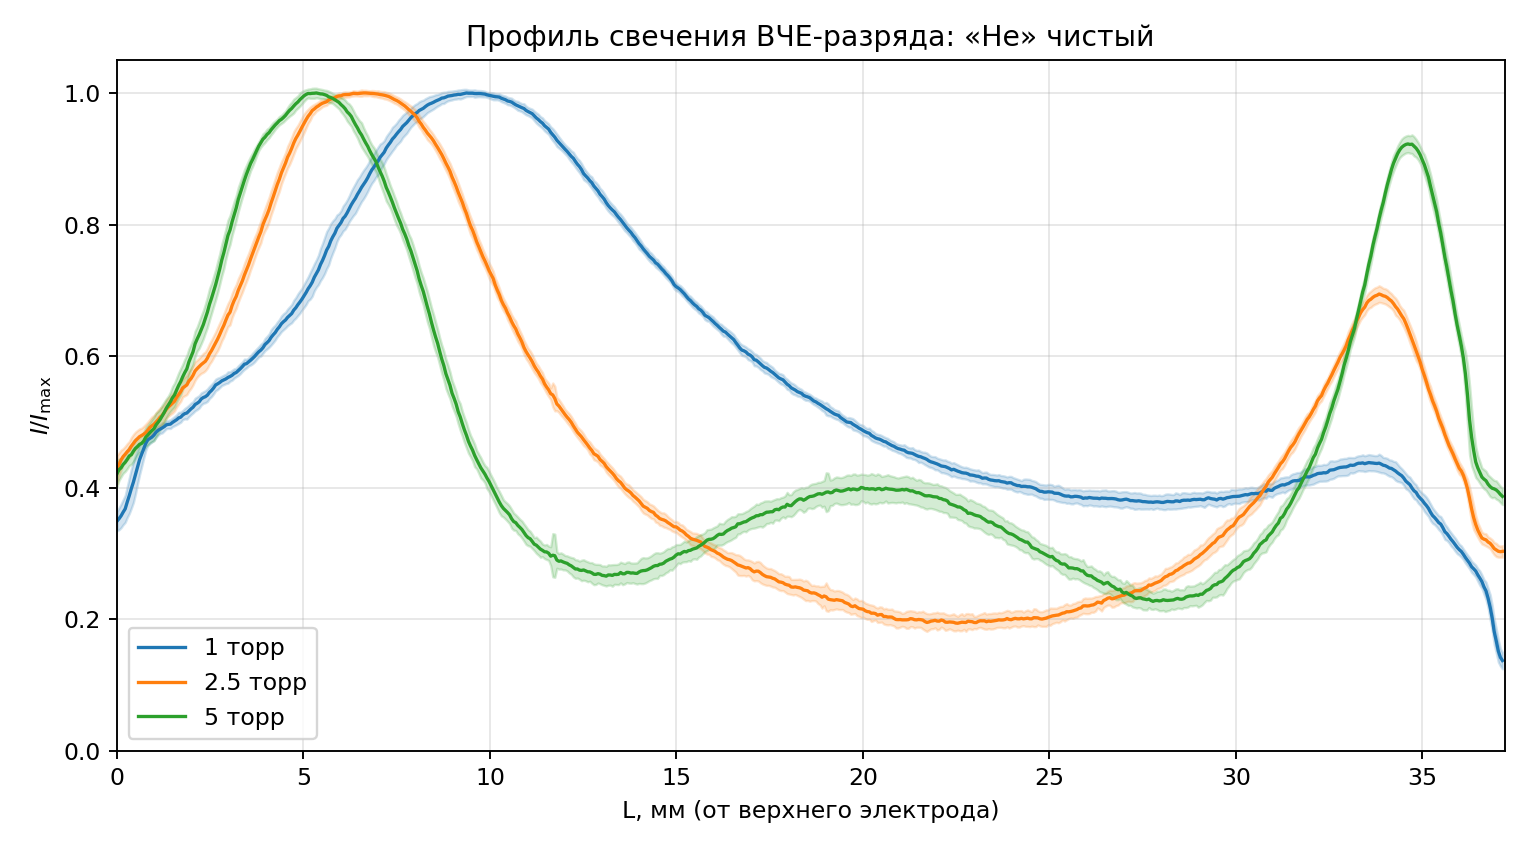
\includegraphics[width=0.85\linewidth]{t2_profile_He.png}
  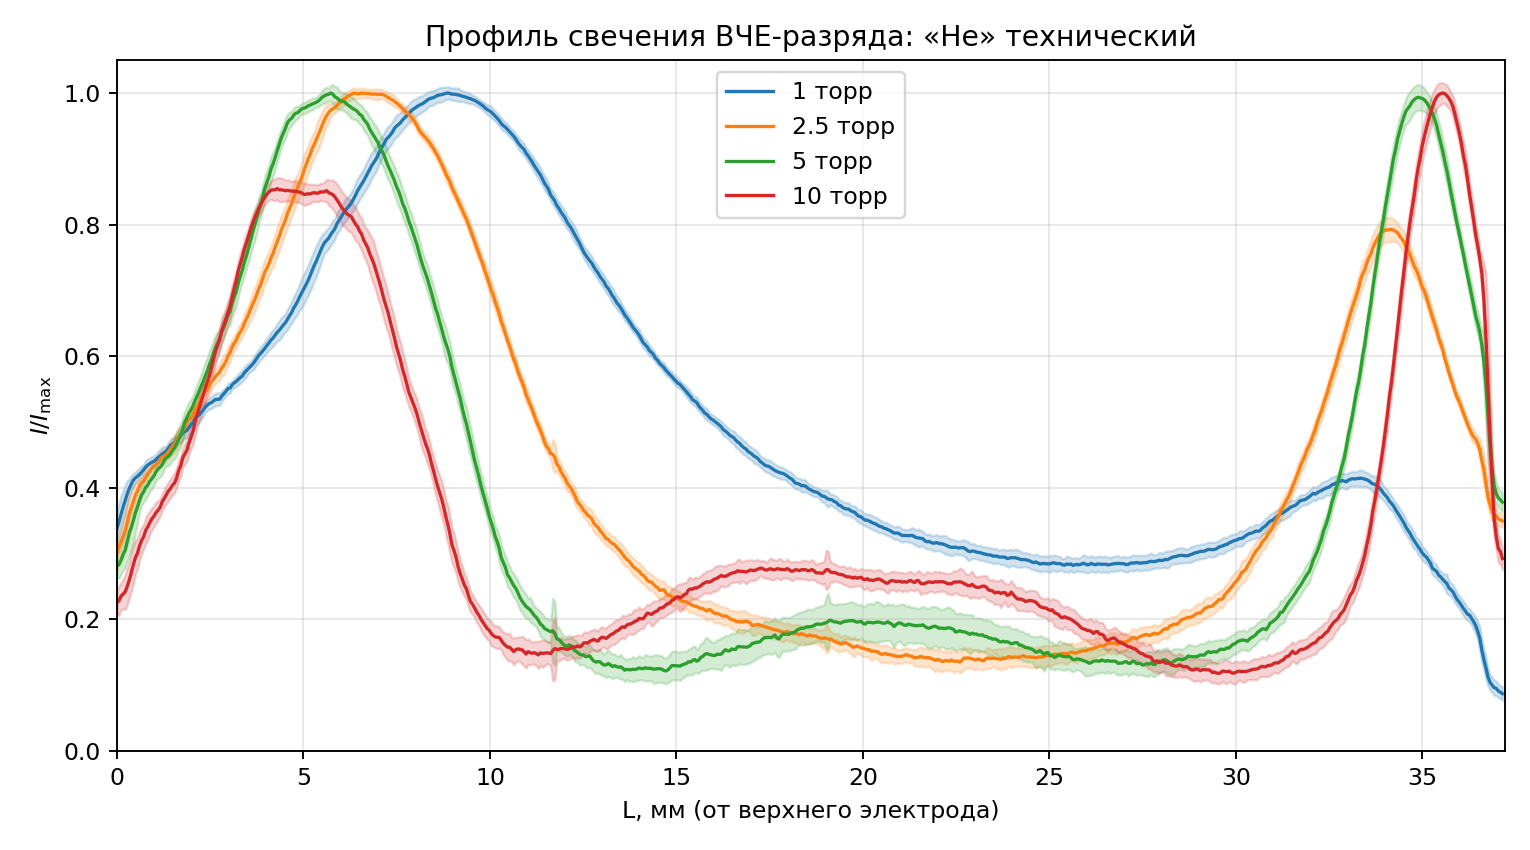
\includegraphics[width=0.85\linewidth]{t2_profile_He_tech.png}
  \caption{Профили свечения ВЧЕ-разряда $I(L)/I_\text{max}$: чистый
  (сверху) и технический (снизу) гелий.}
  \label{fig:t2_prof}
\end{figure}

\begin{figure}[H]
  \centering
  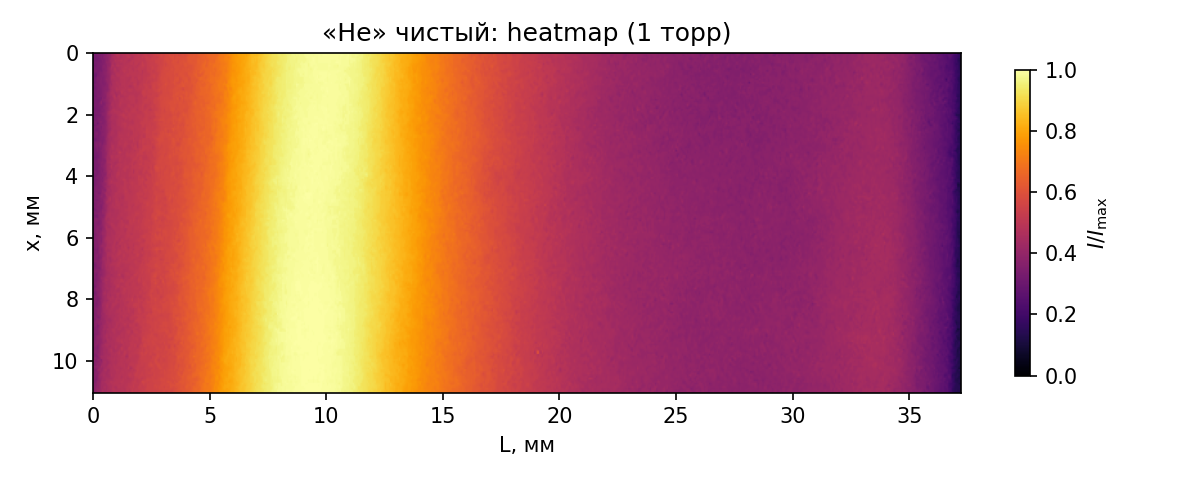
\includegraphics[width=0.49\linewidth]{t2_heatmap_He_1torr.png}\hfill
  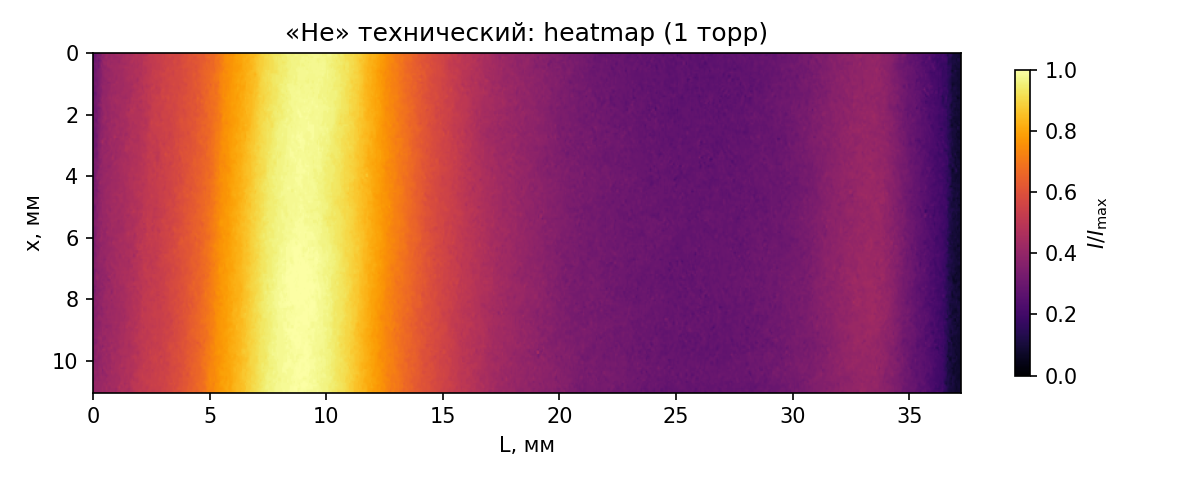
\includegraphics[width=0.49\linewidth]{t2_heatmap_He_tech_1torr.png}\\
  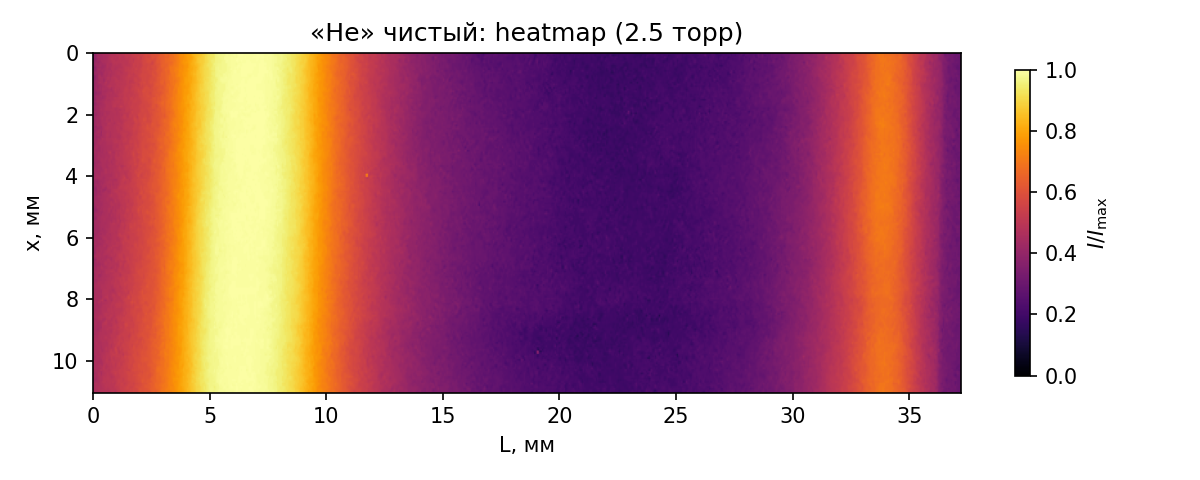
\includegraphics[width=0.49\linewidth]{t2_heatmap_He_2.5torr.png}\hfill
  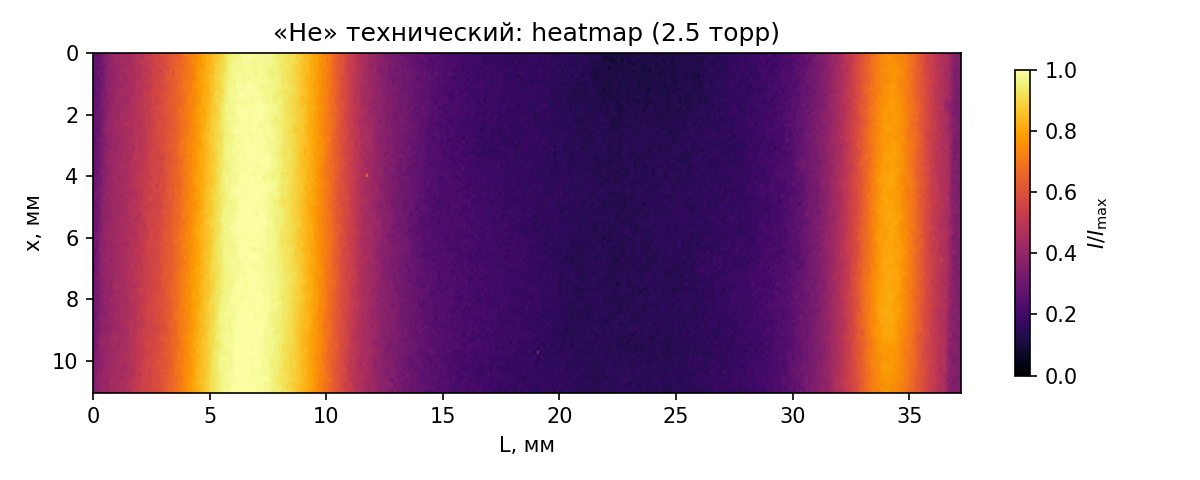
\includegraphics[width=0.49\linewidth]{t2_heatmap_He_tech_2.5torr.png}\\
  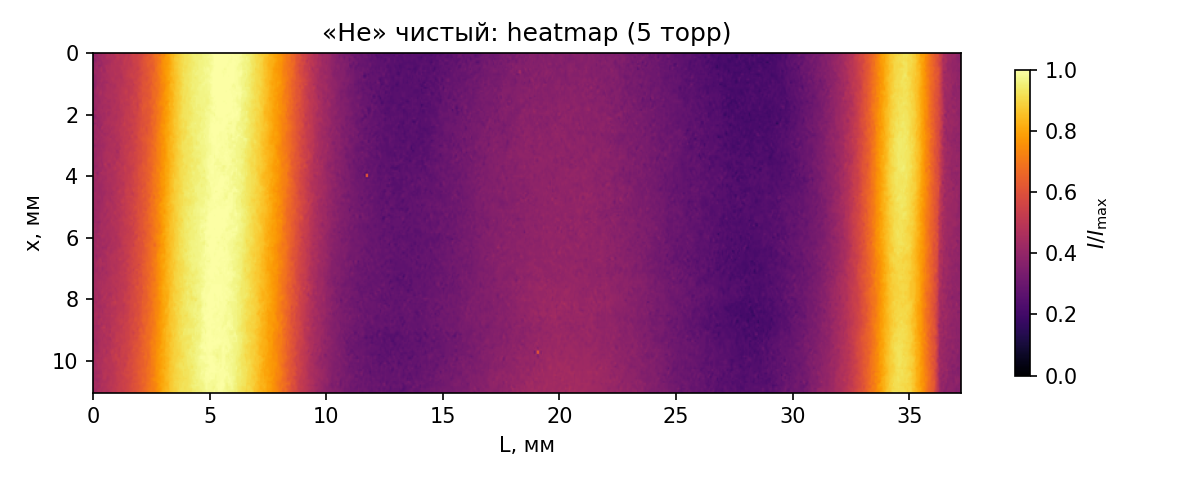
\includegraphics[width=0.49\linewidth]{t2_heatmap_He_5torr.png}\hfill
  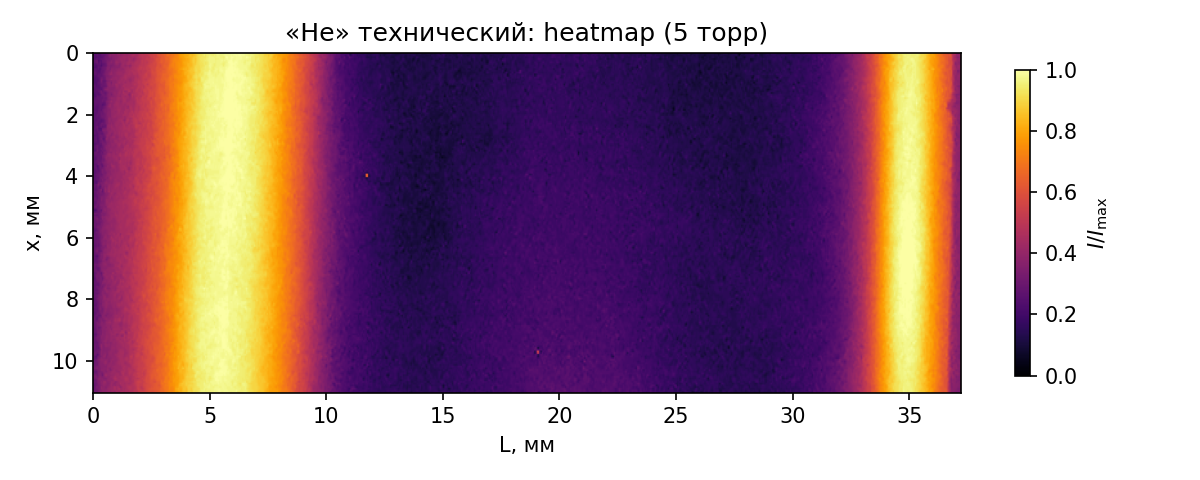
\includegraphics[width=0.49\linewidth]{t2_heatmap_He_tech_5torr.png}\\
  \hfill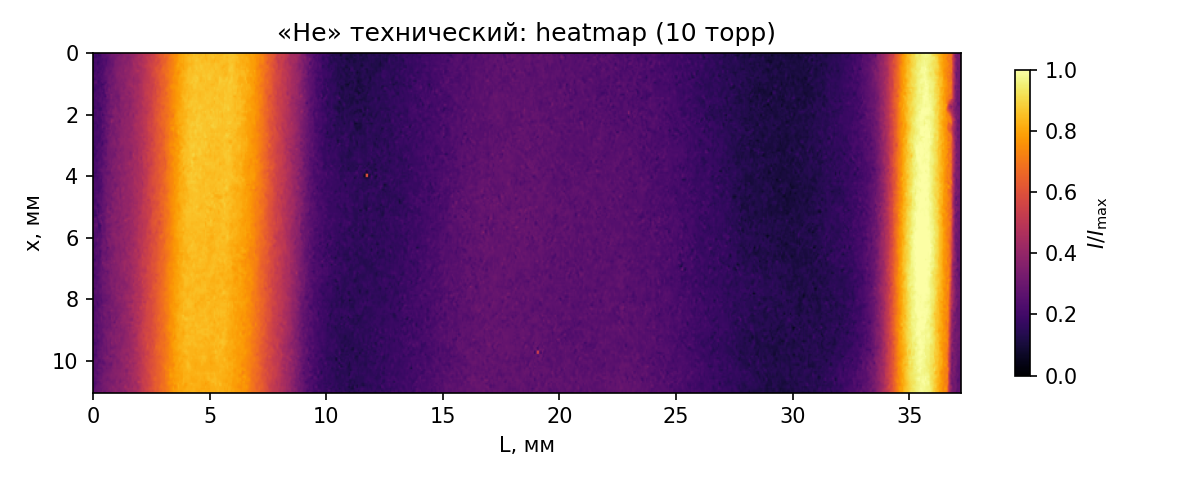
\includegraphics[width=0.49\linewidth]{t2_heatmap_He_tech_10torr.png}
  \caption{Карты яркости межэлектродного промежутка: слева чистый He,
  справа технический; сверху вниз 1; 2,5; 5~Торр, внизу справа ---
  технический He при 10~Торр.}
  \label{fig:t2_heat}
\end{figure}

\begin{table}[H]
  \centering
  \caption{Расстояния от электродов до ярких приэлектродных слоёв
  $d_\text{в}$, $d_\text{н}$ (верхний и нижний электрод), средняя
  относительная яркость центральной половины промежутка
  $\langle I\rangle_\text{ц}/I_\text{max}$ и параметр подобия $P_m L$.}
  \label{tab:t2}
  \begin{tabular}{lccccc}
    \toprule
    Газ & $P_m$, Торр & $d_\text{в}$, мм & $d_\text{н}$, мм &
    $\langle I\rangle_\text{ц}/I_\text{max}$ & $P_m L$, Торр$\cdot$см \\
    \midrule
    He чистый & 1   & 9,5 & ---  & 0,61 & 3,7 \\
    He чистый & 2,5 & 6,6 & 3,3 & 0,32 & 9,3 \\
    He чистый & 5   & 5,4 & 2,6 & 0,33 & 18,6 \\
    \midrule
    He техн. & 1    & 9,0 & 4,1 & 0,49 & 3,7 \\
    He техн. & 2,5  & 6,7 & 3,0 & 0,25 & 9,3 \\
    He техн. & 5    & 5,6 & 2,3 & 0,18 & 18,6 \\
    He техн. & 10   & 4,8 & 1,7 & 0,22 & 37,2 \\
    \bottomrule
  \end{tabular}
\end{table}

\paragraph{Наблюдения во время опыта.}
При $P_m = 3{,}9$~Торр в чистом гелии и $3{,}5$~Торр в техническом
появлялась дополнительная страта --- светящаяся зона в середине
промежутка. При дальнейшем повышении давления в техническом гелии
центральный слой раздваивался (появлялась тонкая тёмная полоса).

\paragraph{Переход $\alpha\to\gamma$.}
Будем считать моментом перехода появление центральной светящейся зоны,
отделённой тёмными слоями от ярких приэлектродных слоёв (картина
$\gamma$-формы). Тогда
\begin{equation}
  (P_m L)_\text{He} = 3{,}9 \cdot 3{,}72 = 14{,}5 \pm 0{,}4~\text{Торр$\cdot$см},
  \qquad
  (P_m L)_\text{He техн} = 3{,}5 \cdot 3{,}72 = 13{,}0 \pm 0{,}4~\text{Торр$\cdot$см}
\end{equation}
(погрешность учитывает $\Delta P = 0{,}1$~Торр и $\Delta L = 0{,}2$~мм).

\subsection{Красный канал: вклад азота}
\label{sec:red}

Примесь воздуха светится в основном полосами азота: в ультрафиолете
(315--380~нм) и в красной области (580--780~нм). Ультрафиолет камера не
регистрирует, поэтому вклад азота на снимках может проявиться только в
красном канале. Но в красный канал попадают и яркие линии гелия
(667,8; 706,5; 728~нм), поэтому профили по красному каналу построены
для обоих газов: чистый He служит контролем (рис.~\ref{fig:t2_red}).

\begin{figure}[H]
  \centering
  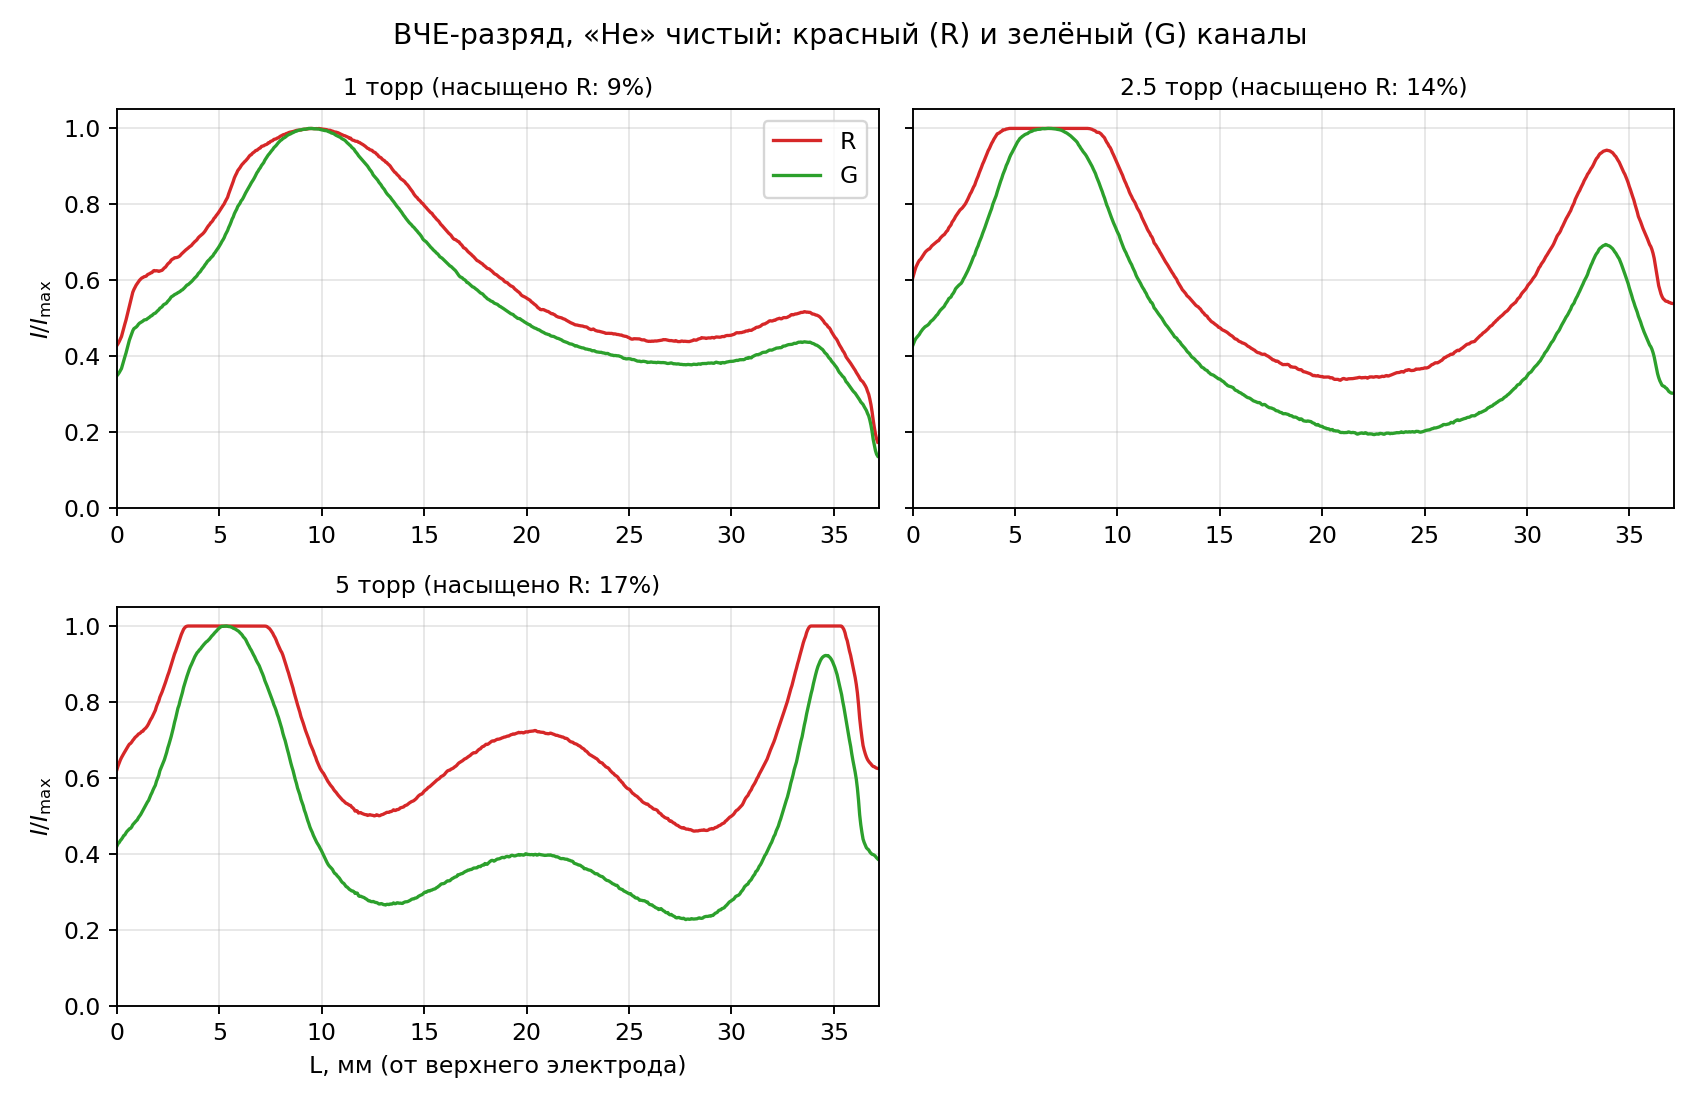
\includegraphics[width=0.95\linewidth]{t2_profile_red_He.png}
  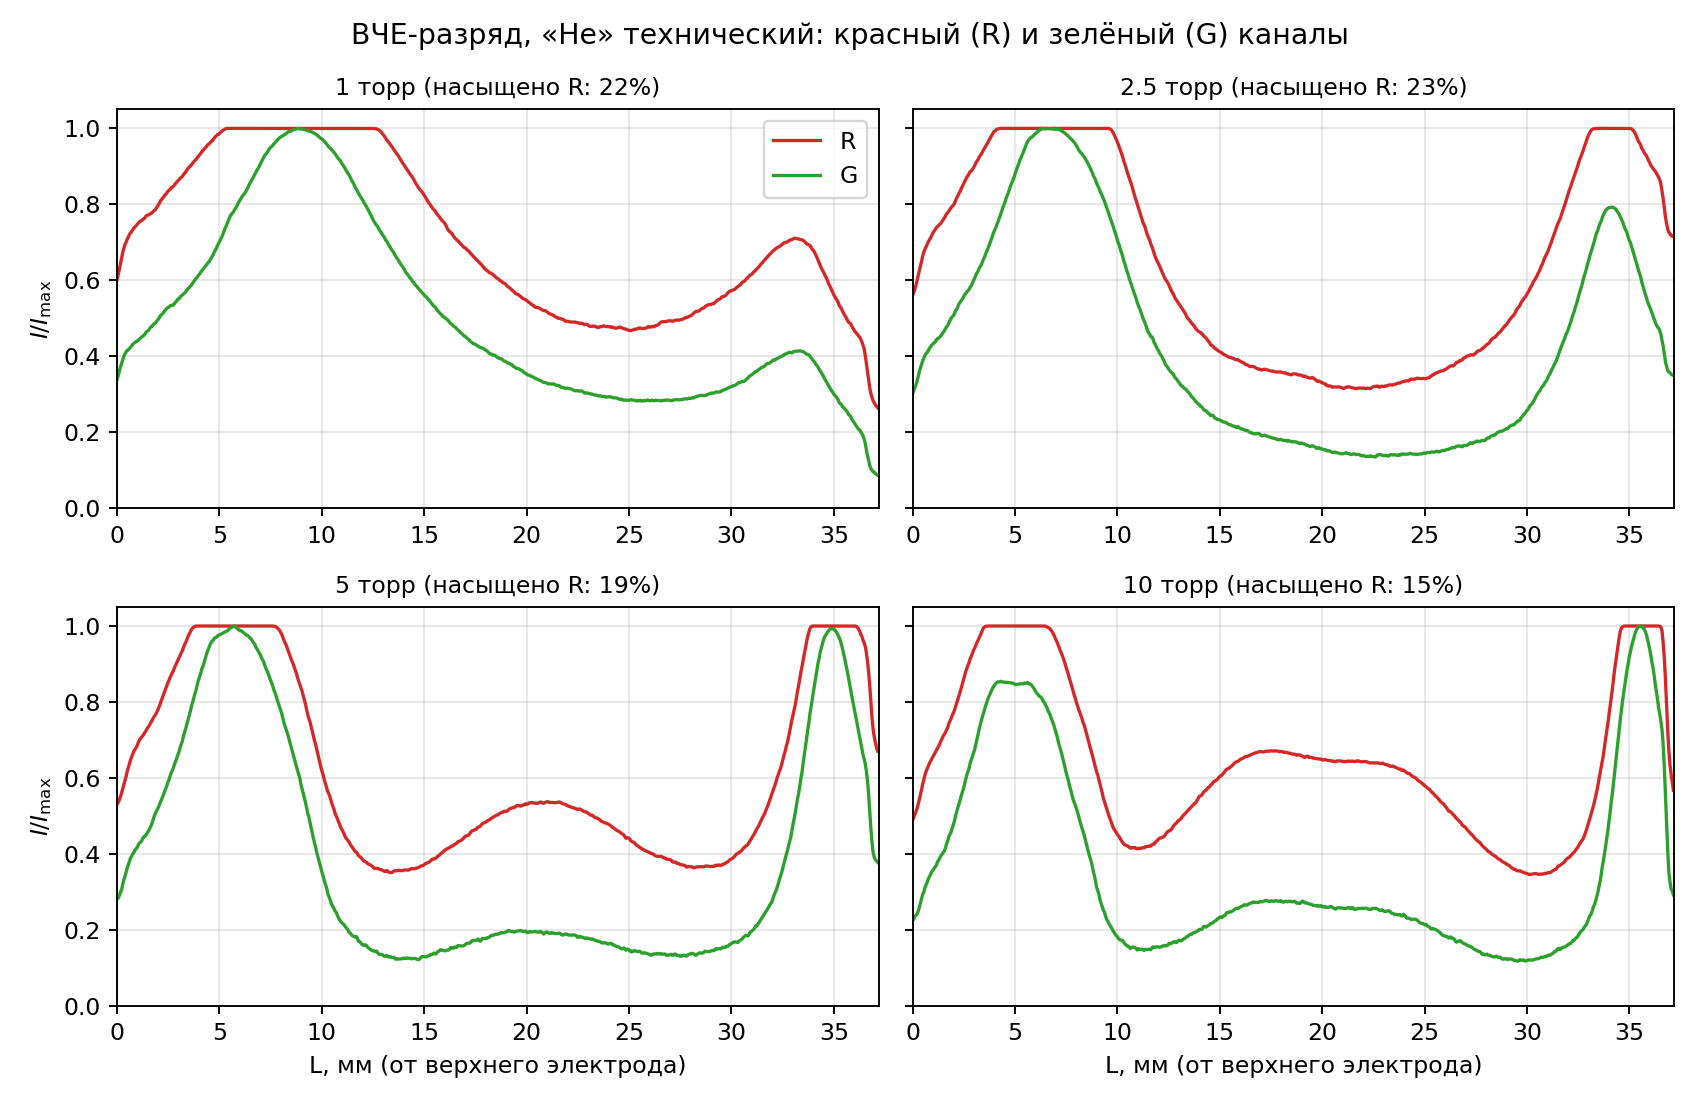
\includegraphics[width=0.95\linewidth]{t2_profile_red_He_tech.png}
  \caption{Профили $I(L)$ ВЧЕ-разряда по красному (R) и зелёному (G)
  каналам, каждый нормирован на свой максимум: чистый He (сверху) и
  технический He (снизу). В заголовках --- доля насыщенных пикселей
  красного канала в полоске.}
  \label{fig:t2_red}
\end{figure}

\begin{table}[H]
  \centering
  \caption{Средняя относительная яркость центральной половины промежутка
  в красном и зелёном каналах.}
  \label{tab:red}
  \begin{tabular}{lcccc}
    \toprule
    Газ & $P_m$, Торр & $\langle I_R\rangle_\text{ц}/I_{R,\max}$ &
    $\langle I_G\rangle_\text{ц}/I_{G,\max}$ & насыщено R \\
    \midrule
    He чистый & 1   & 0,67 & 0,61 & 9\% \\
    He чистый & 2,5 & 0,48 & 0,32 & 14\% \\
    He чистый & 5   & 0,61 & 0,33 & 17\% \\
    \midrule
    He техн.  & 1   & 0,68 & 0,49 & 22\% \\
    He техн.  & 2,5 & 0,45 & 0,25 & 23\% \\
    He техн.  & 5   & 0,46 & 0,18 & 19\% \\
    He техн.  & 10  & 0,57 & 0,22 & 15\% \\
    \bottomrule
  \end{tabular}
\end{table}

Наблюдения (табл.~\ref{tab:red}):
\begin{itemize}
  \item В красном канале центр промежутка ярче, чем в зелёном, во всех
        режимах, кроме чистого He при 1~Торр, где каналы почти совпадают
        (0,67 и 0,61). Там, по спектрам, азота меньше всего.
  \item В чистом He при 5~Торр разница такая же большая, как в
        техническом (0,61 против 0,33). Это согласуется со спектрами: при
        5~Торр полосы азота сильны и в <<чистом>> гелии
        (п.~\ref{sec:spectra}).
  \item Часть разницы --- артефакт: в красном канале насыщено 9--23\,\%
        пикселей, яркие приэлектродные слои срезаны, $I_{R,\max}$
        занижен, и относительная яркость центра завышена.
\end{itemize}
Поэтому красный канал даёт только качественное подтверждение: там, где
спектры показывают сильные полосы азота, центр промежутка в красном
канале заметно ярче, чем в зелёном. Состав излучения определяем по
спектрам, а не по каналам камеры.

\subsection{Оптическая спектроскопия}
\label{sec:spectra}

Спектры записаны спектрометром AvaSpec-2048-2 (программа AvaSoft 7.5.3)
с двумя линейками: Master (красная кривая, примерно 180--735~нм) и
Slave (синяя, 600--1100~нм). На графиках спектров участок выше 600~нм
показан по линейке Slave; на графиках проверки прозрачности
(рис.~\ref{fig:transp}) Master показана целиком, до 735~нм. Мощность
разряда 50~Вт, время накопления 2,5--4~с (указано в заголовке каждого
графика). Спектры не исправлены на спектральную чувствительность, а
чувствительность линеек различна (одна и та же линия 668~нм на Slave
примерно в 3 раза выше, чем на Master, рис.~\ref{fig:transp}).
Поэтому высоты пиков сравниваются только в пределах одной линейки.
Пунктиром отмечены длины волн найденных пиков.

\begin{figure}[H]
  \centering
  \begin{subfigure}{0.49\linewidth}
    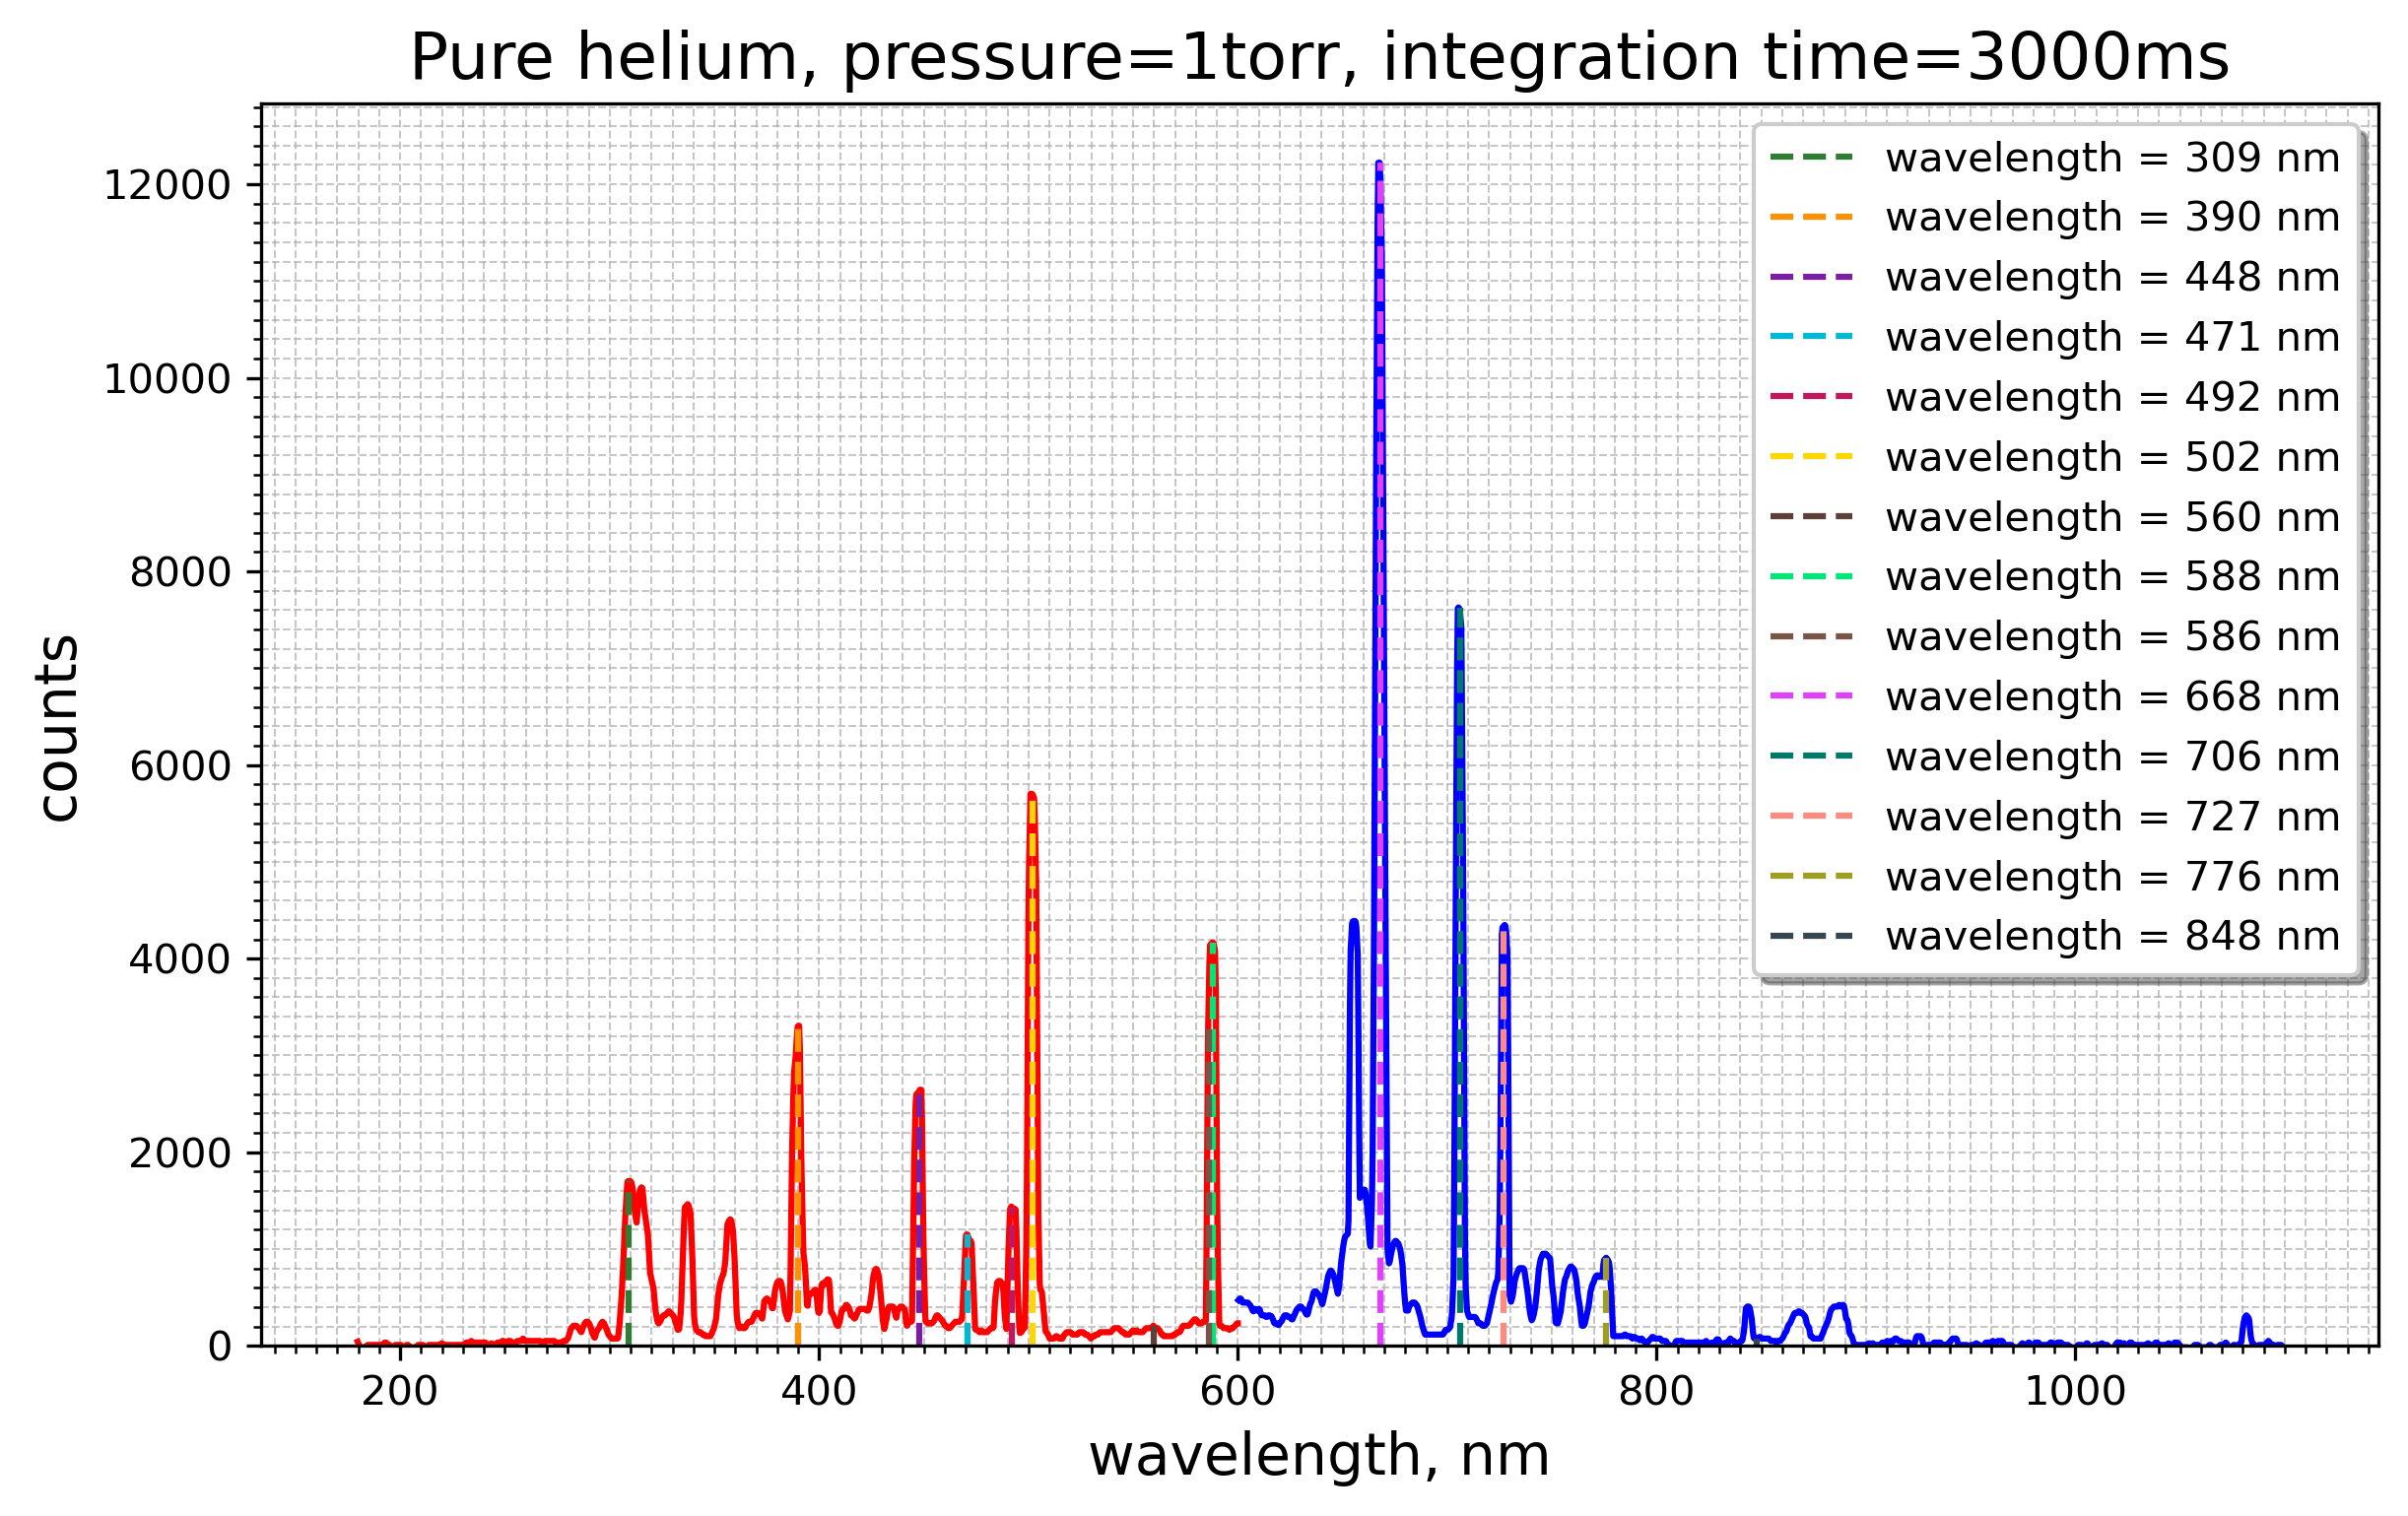
\includegraphics[width=\linewidth]{spec_He_1torr.png}
    \caption{чистый He, 1~Торр}
  \end{subfigure}\hfill
  \begin{subfigure}{0.49\linewidth}
    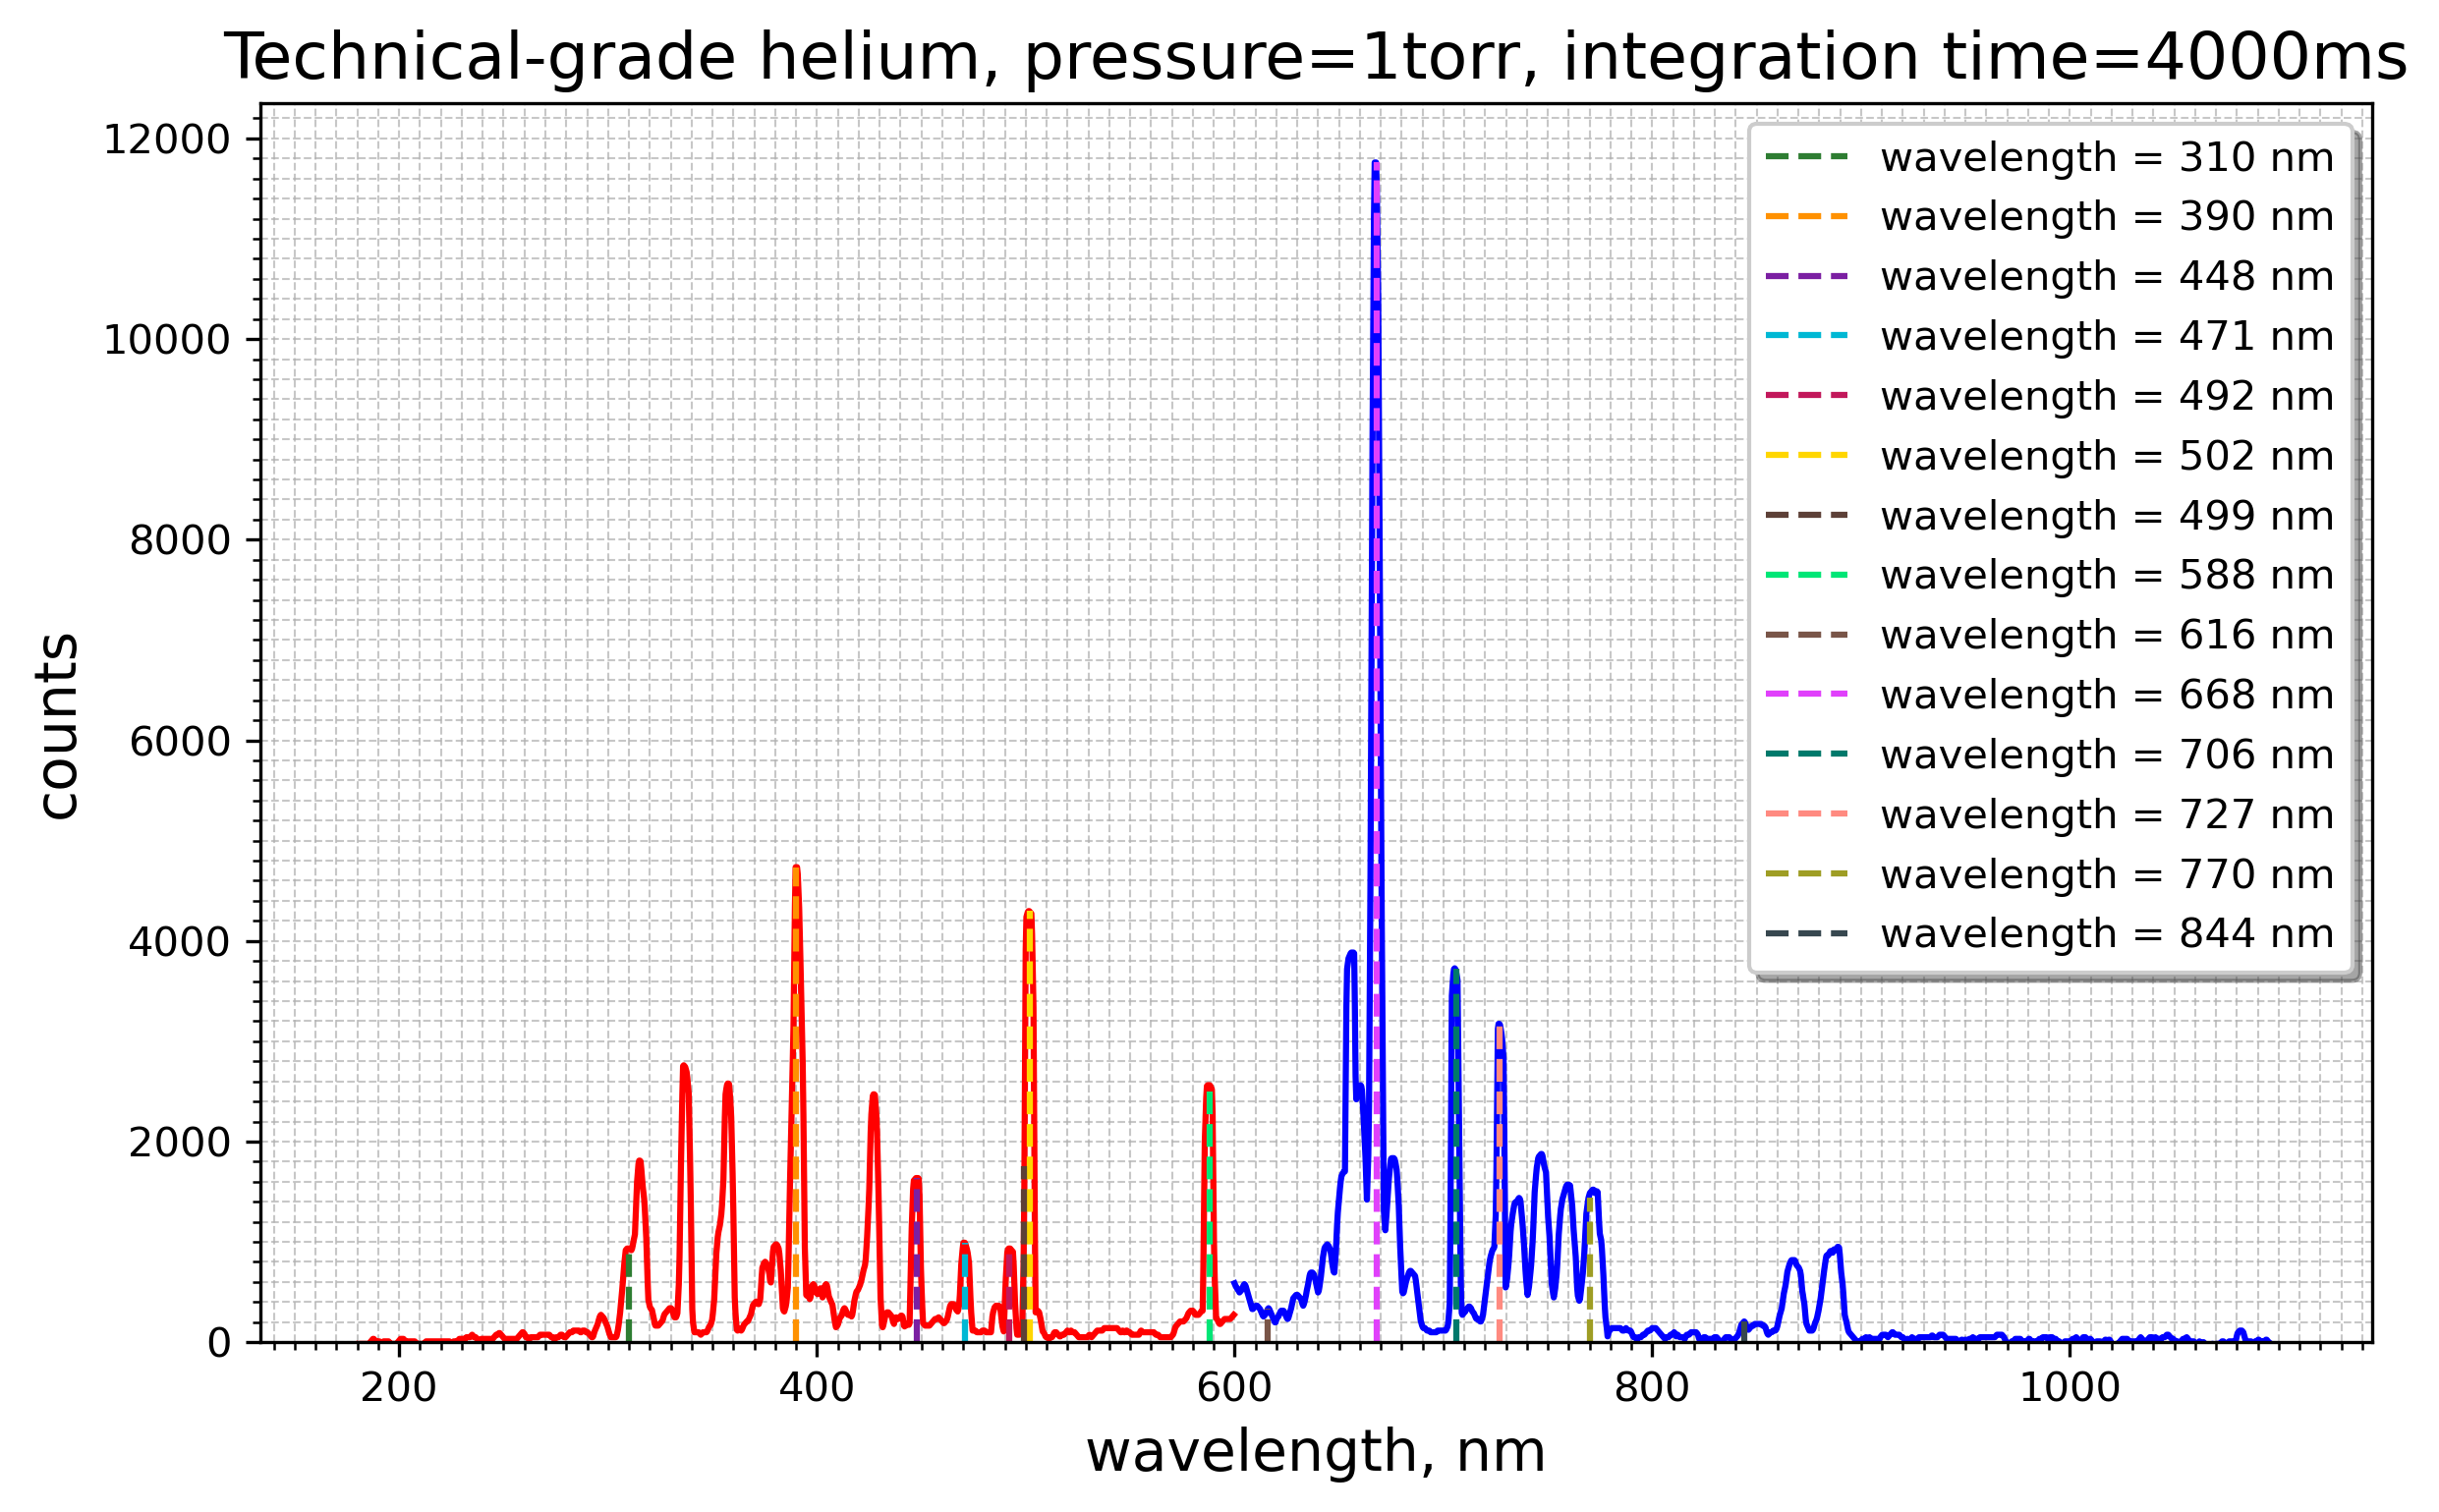
\includegraphics[width=\linewidth]{spec_He_tech_1torr.png}
    \caption{технический He, 1~Торр}
  \end{subfigure}\\[4pt]
  \begin{subfigure}{0.49\linewidth}
    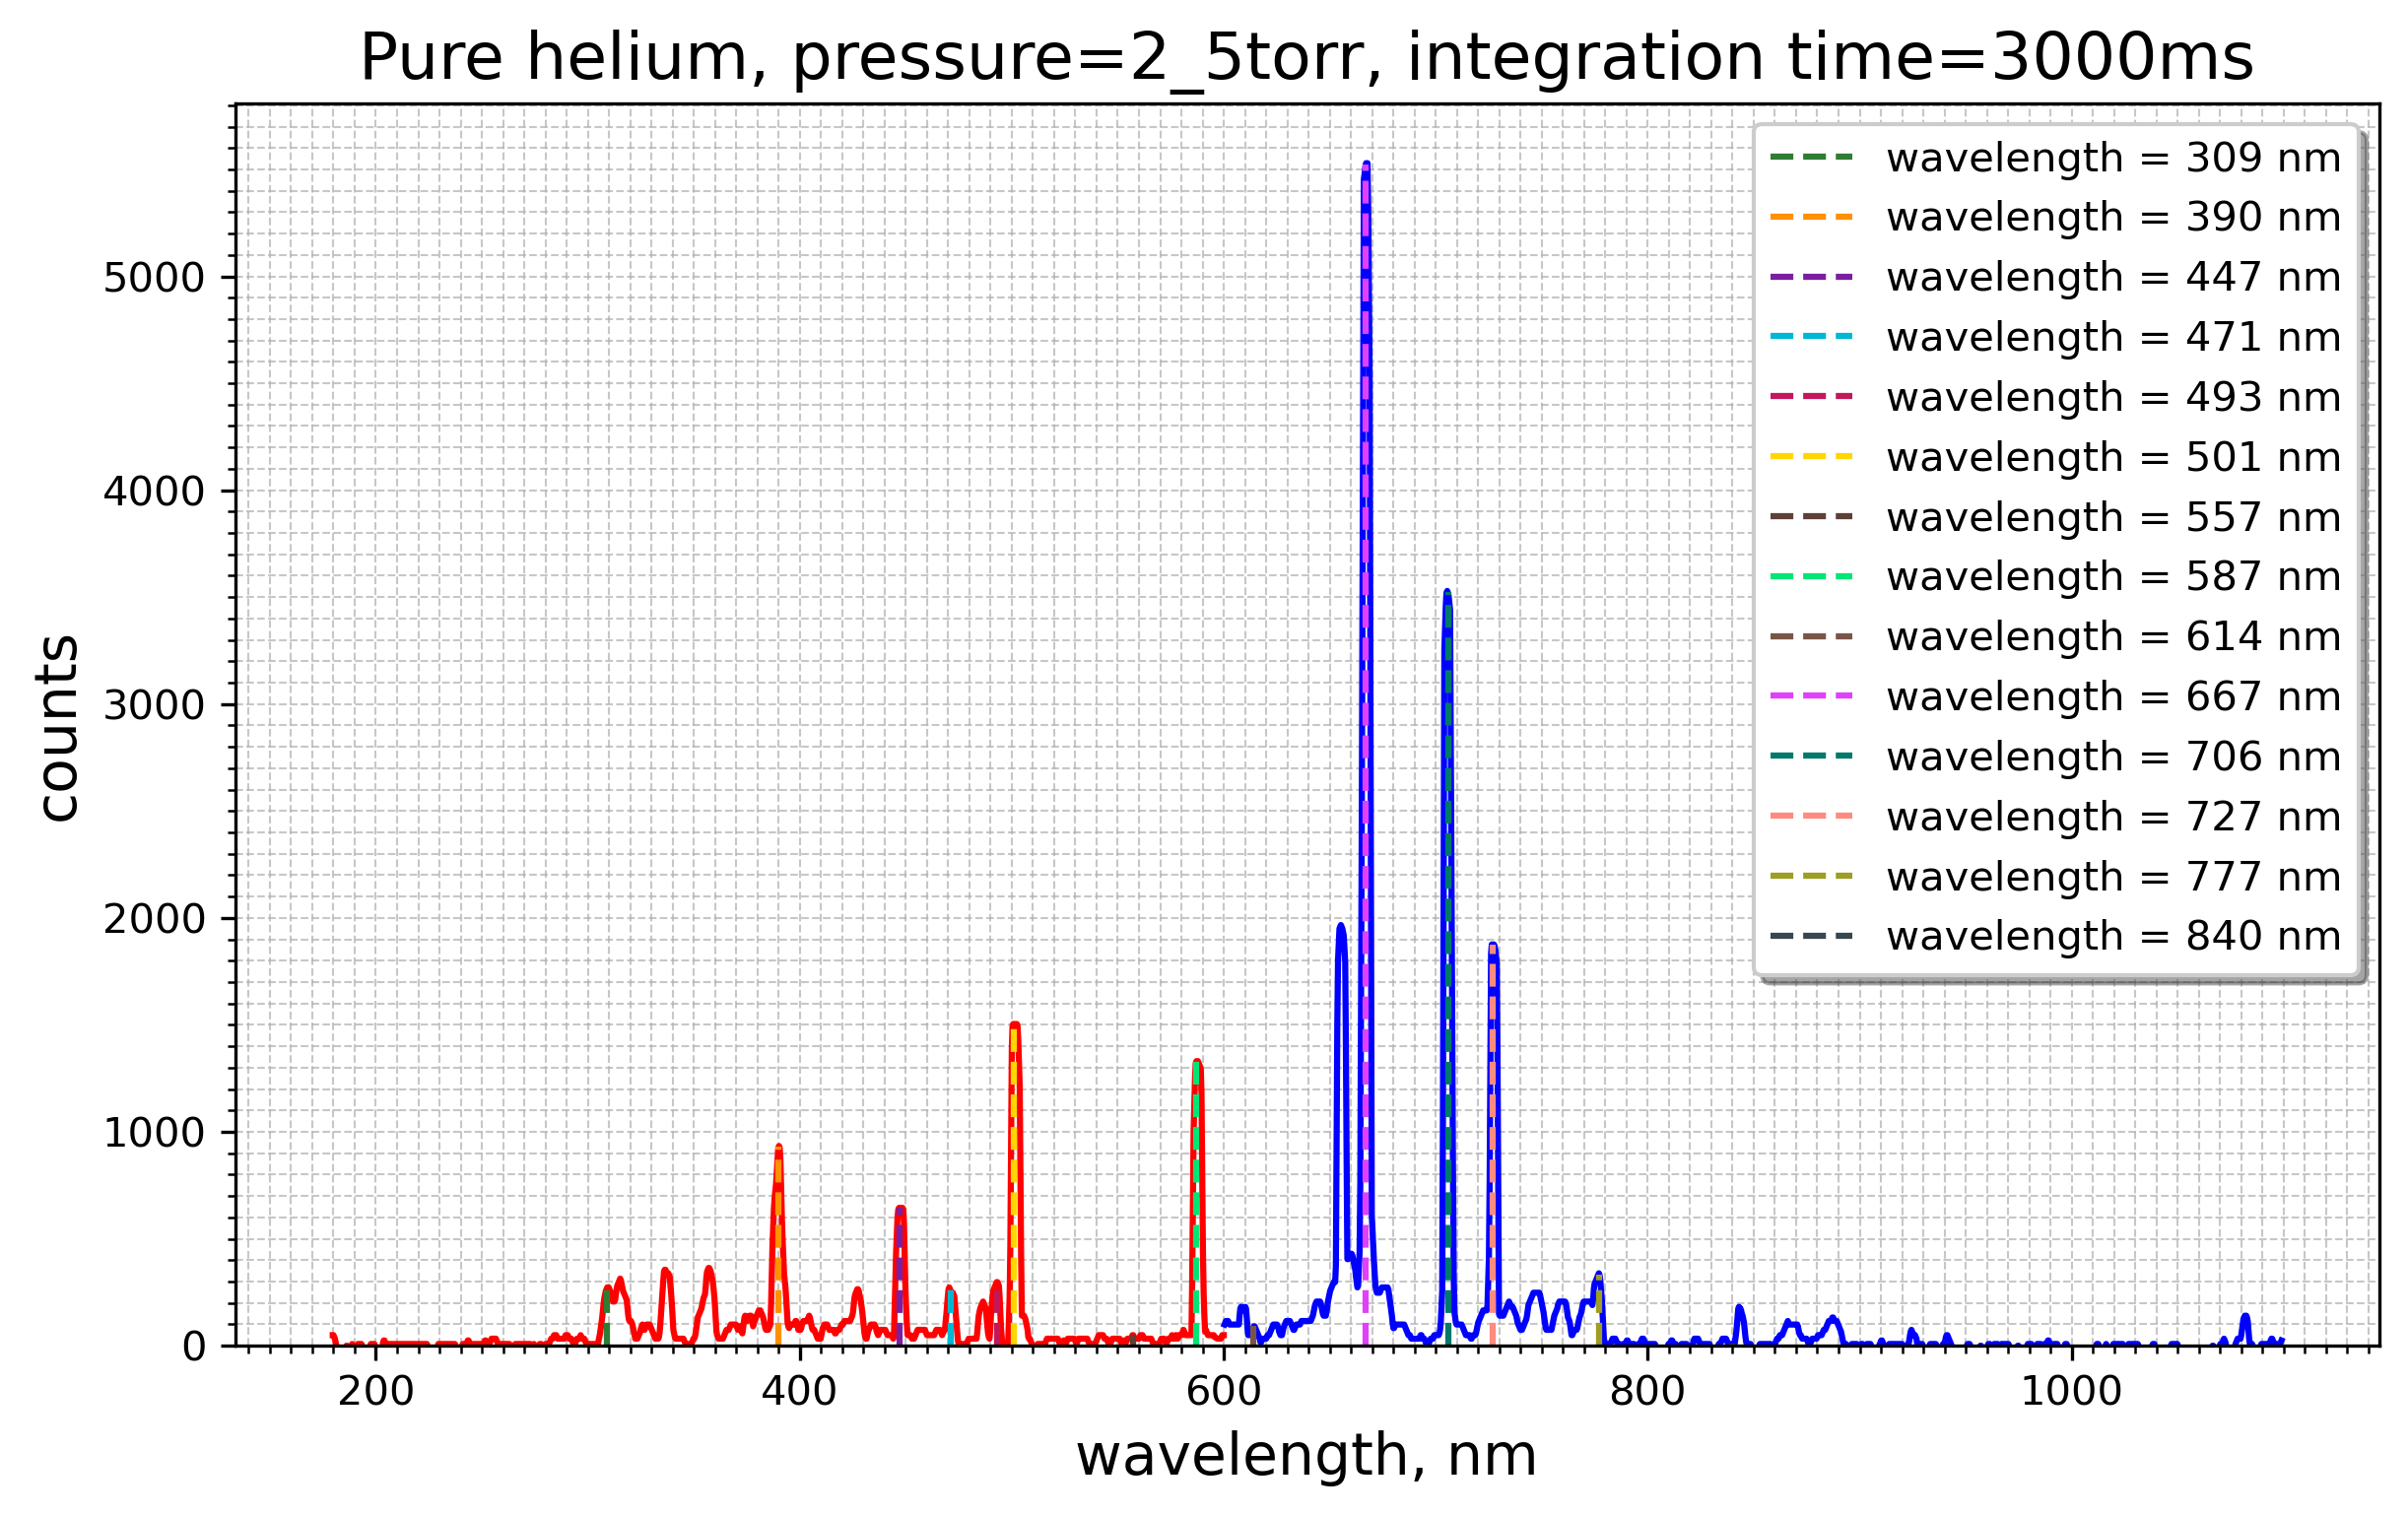
\includegraphics[width=\linewidth]{spec_He_2.5torr.png}
    \caption{чистый He, 2,5~Торр}
  \end{subfigure}\hfill
  \begin{subfigure}{0.49\linewidth}
    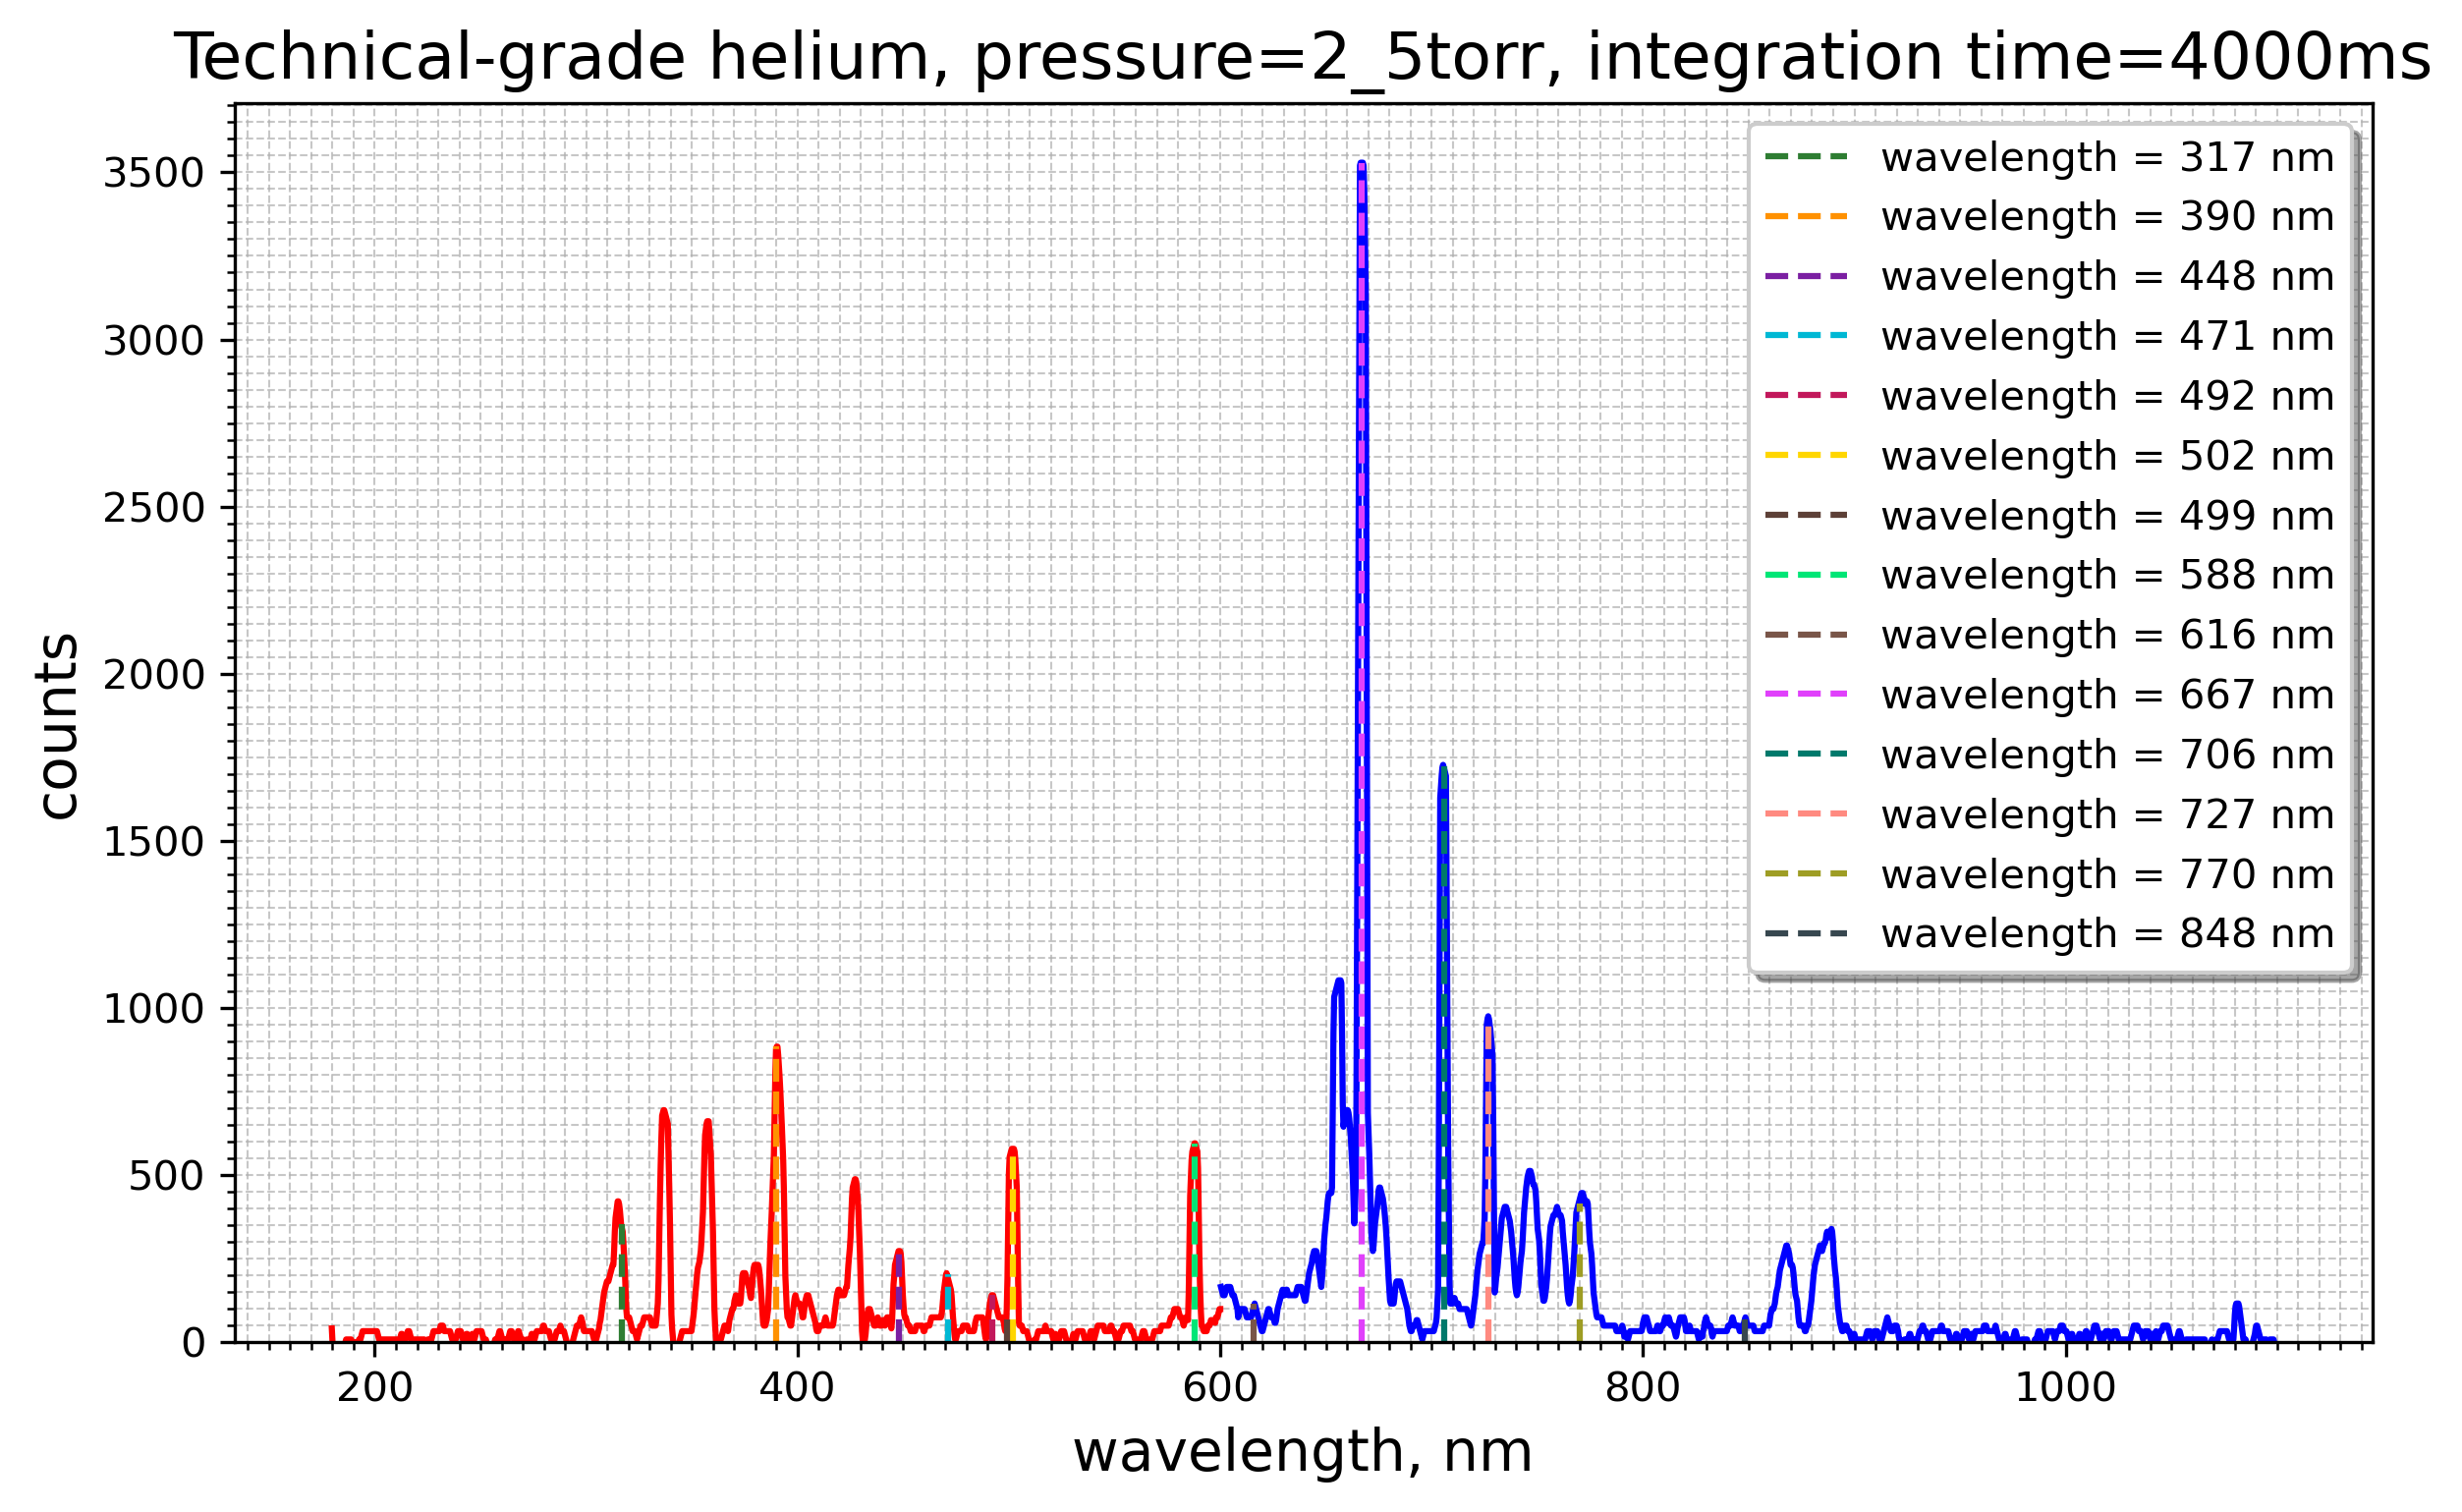
\includegraphics[width=\linewidth]{spec_He_tech_2.5torr.png}
    \caption{технический He, 2,5~Торр}
  \end{subfigure}\\[4pt]
  \begin{subfigure}{0.49\linewidth}
    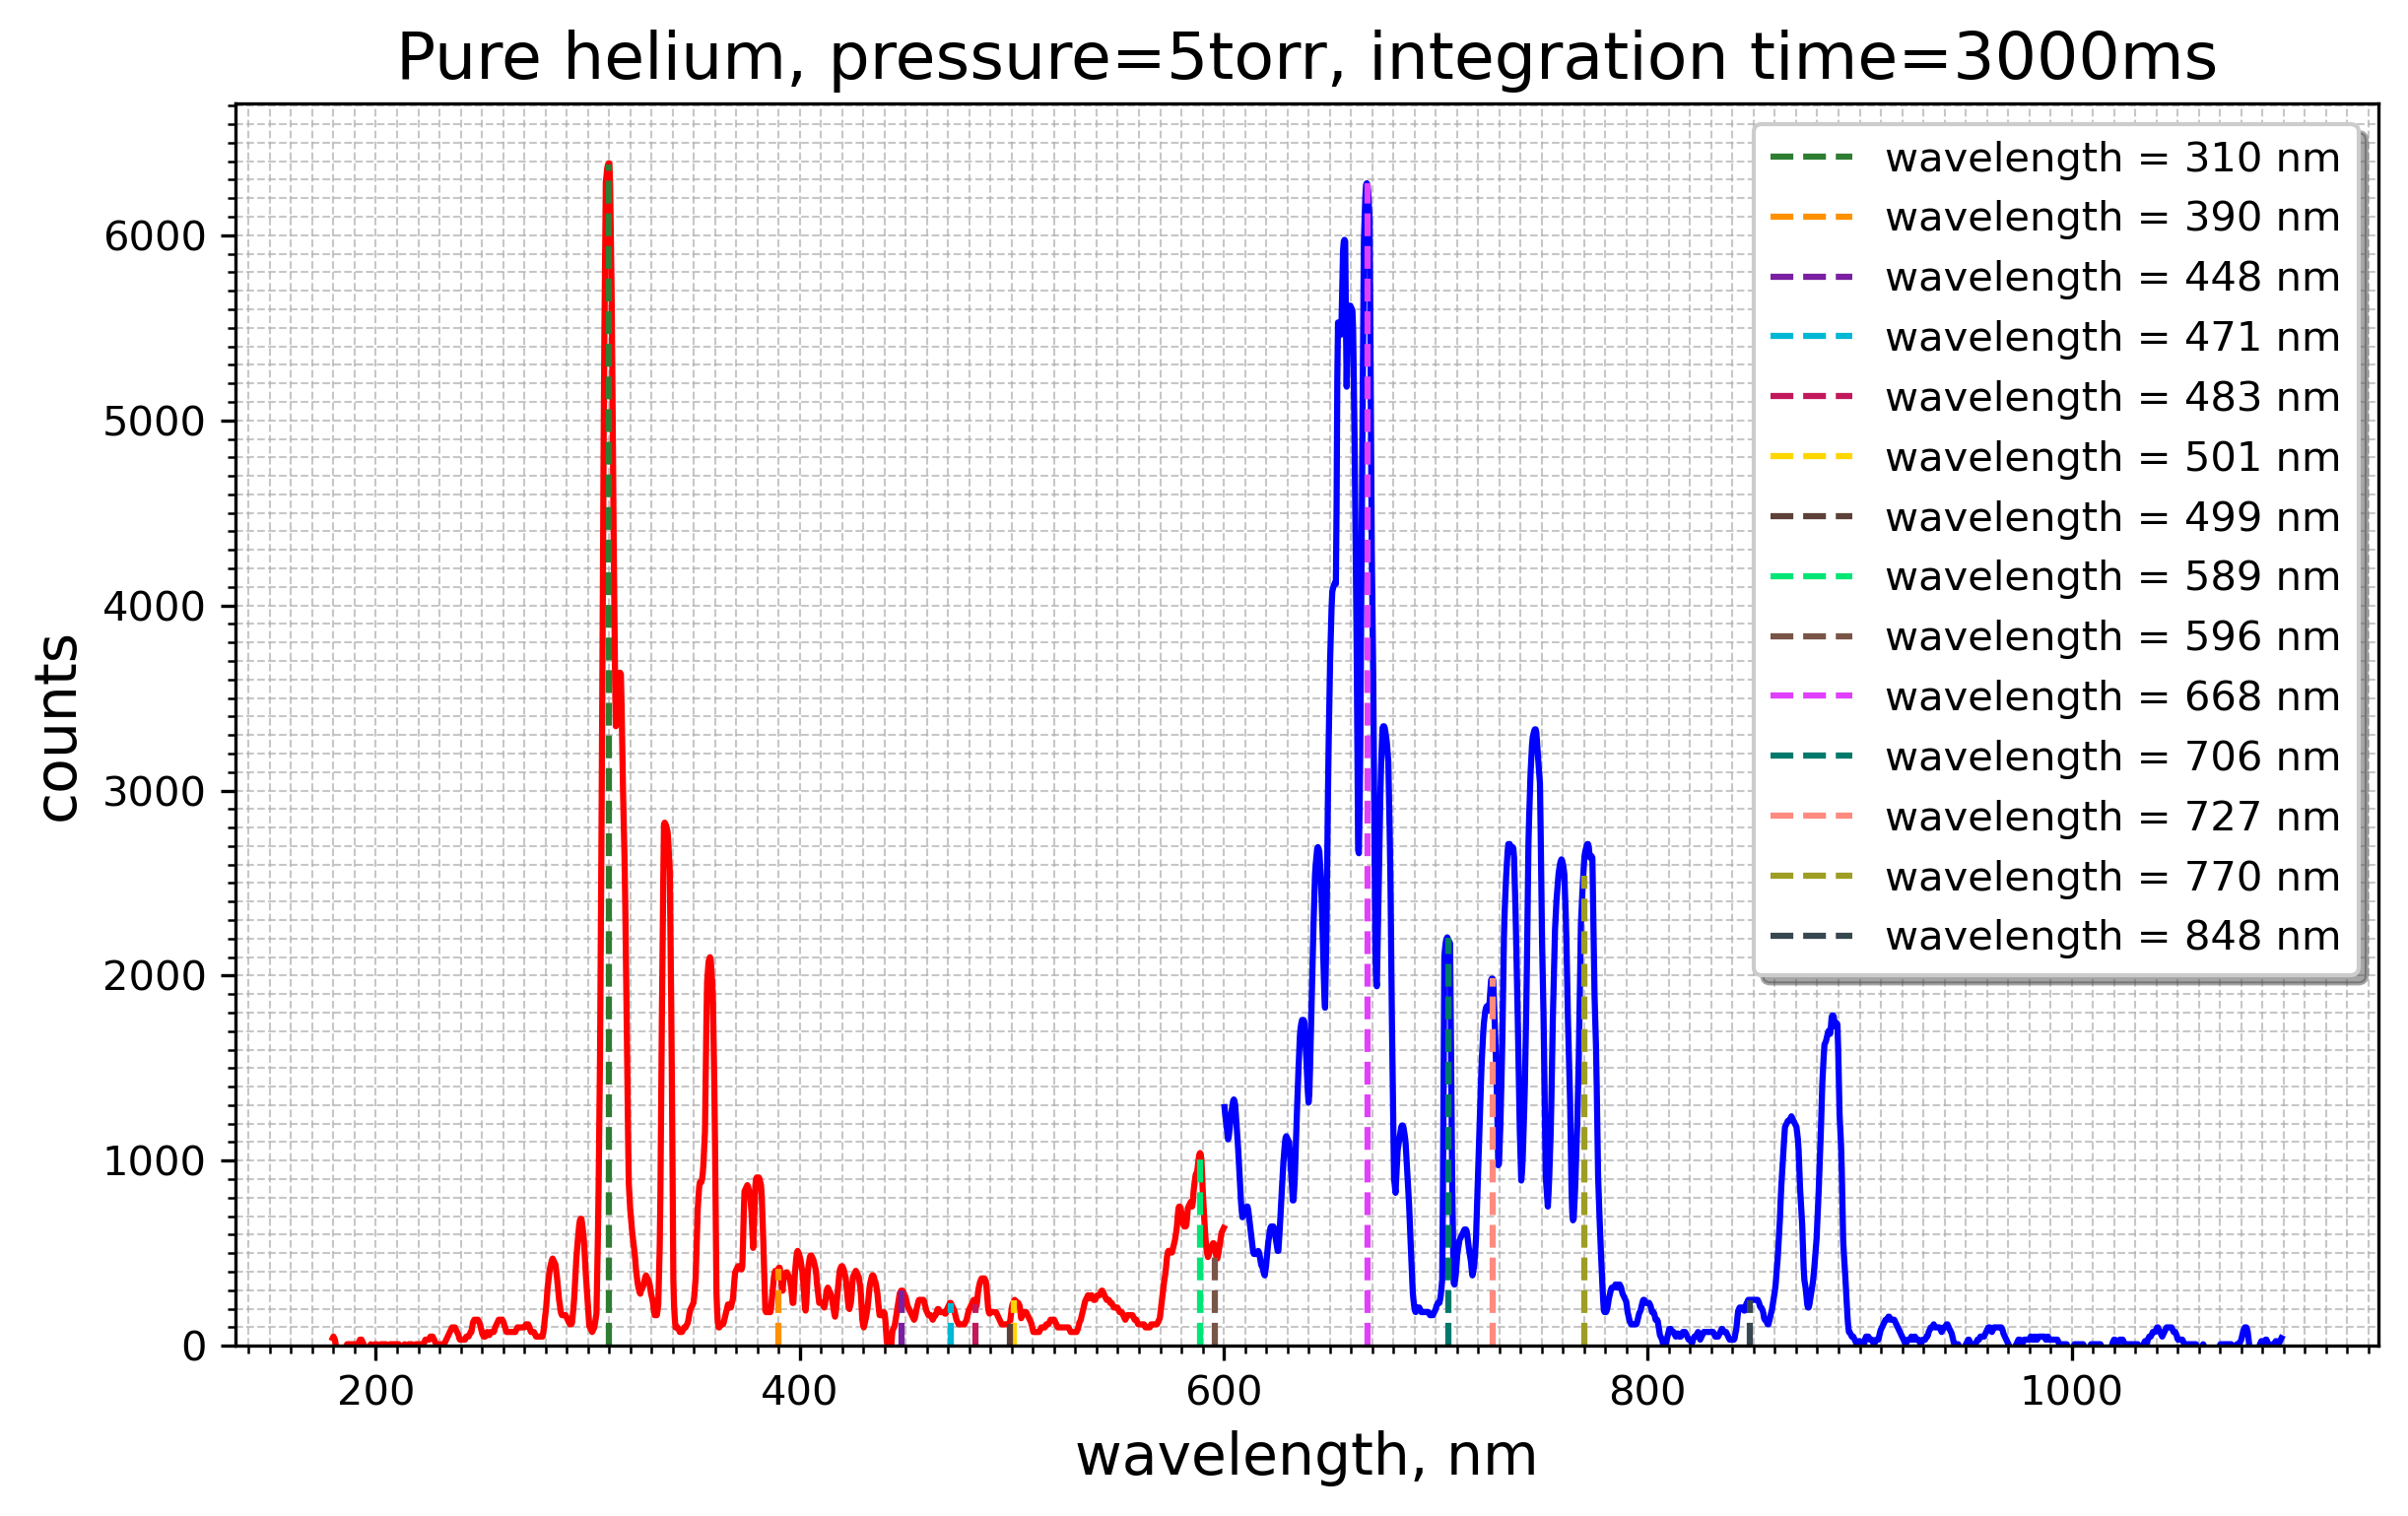
\includegraphics[width=\linewidth]{spec_He_5torr.png}
    \caption{чистый He, 5~Торр}
  \end{subfigure}\hfill
  \begin{subfigure}{0.49\linewidth}
    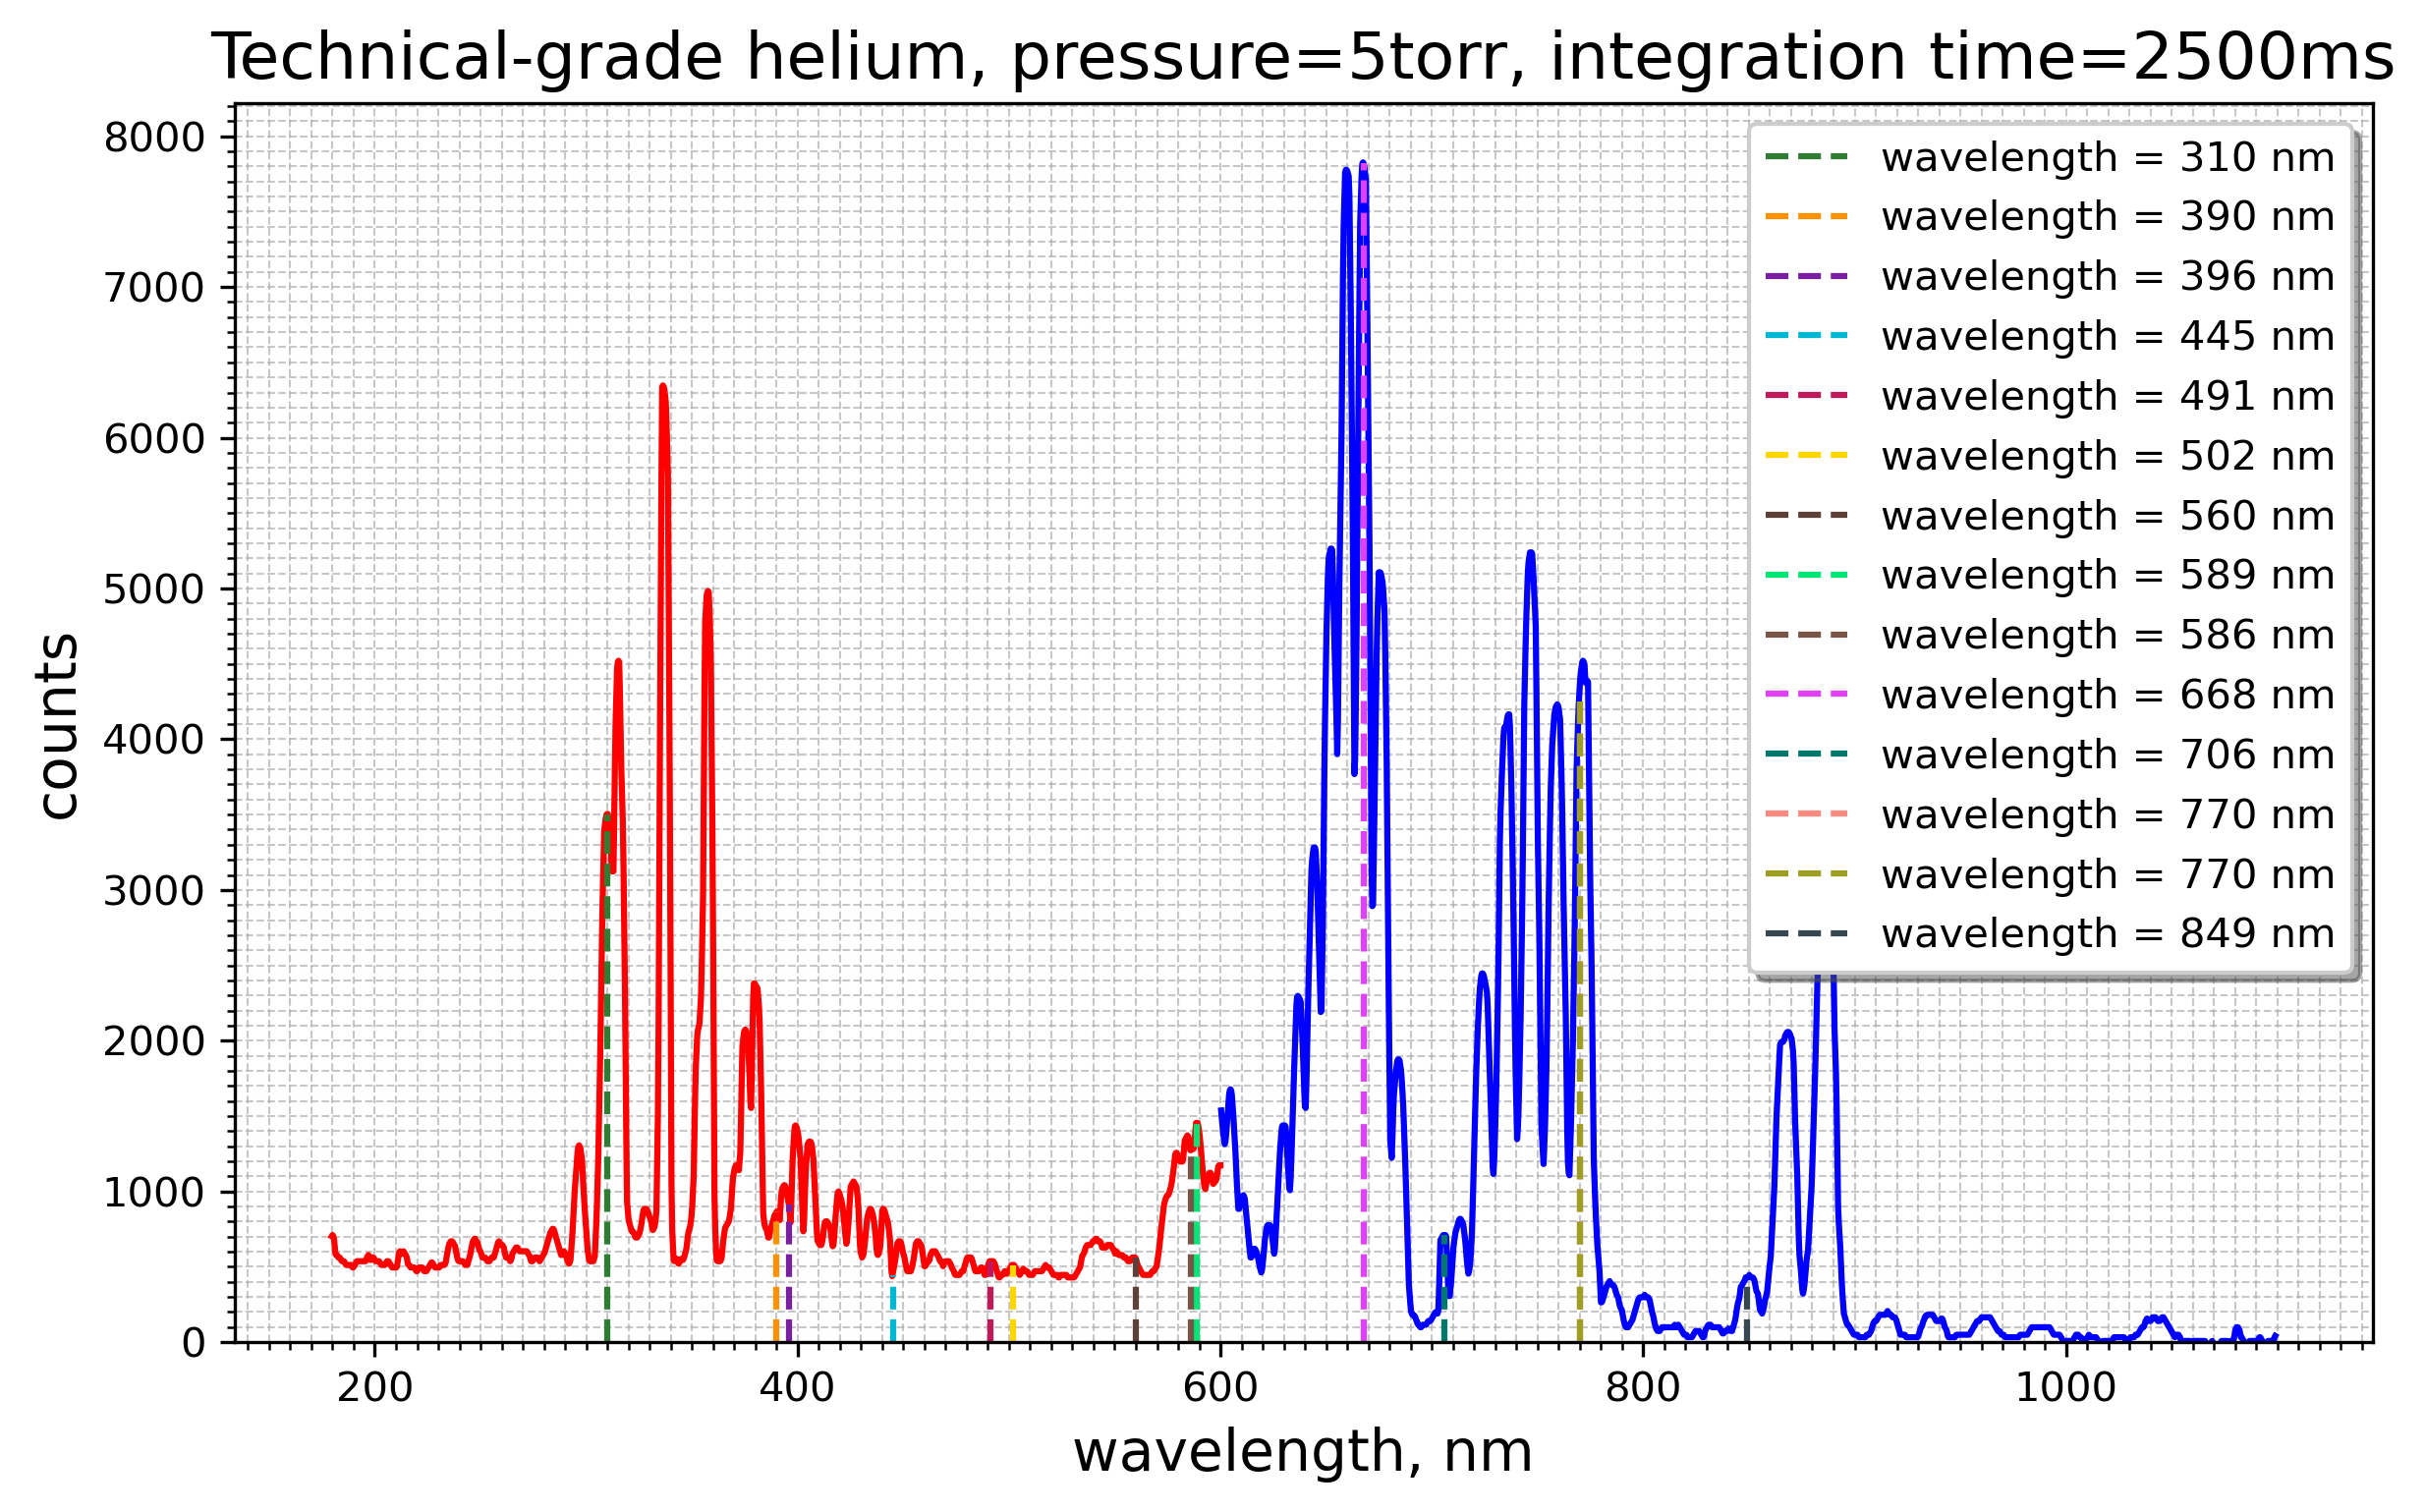
\includegraphics[width=\linewidth]{spec_He_tech_5torr.png}
    \caption{технический He, 5~Торр}
  \end{subfigure}
  \caption{Спектры излучения ВЧЕ-разряда (без подсветки лампой).}
  \label{fig:spectra}
\end{figure}

\paragraph{Как определить, что светится.}
Каждое вещество светится на своих длинах волн, поэтому пики
определяются сравнением с опубликованными спектрами
(рис.~\ref{fig:ident}): эталонным спектром гелия~[4] и спектром плазмы в
гелии с примесью воздуха в области 300--440~нм~[3]. Наши спектры имеют
те же пики.

\begin{figure}[H]
  \centering
  \begin{subfigure}{0.49\linewidth}
    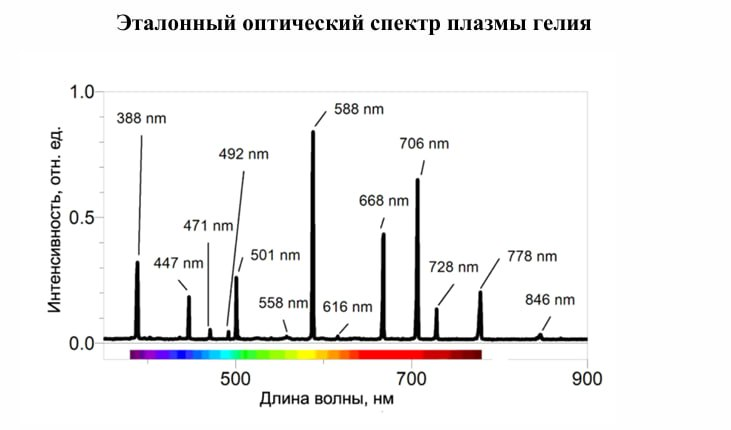
\includegraphics[width=\linewidth]{spec_ident_He.png}
    \caption{эталонный спектр гелия~[4]}
  \end{subfigure}\hfill
  \begin{subfigure}{0.49\linewidth}
    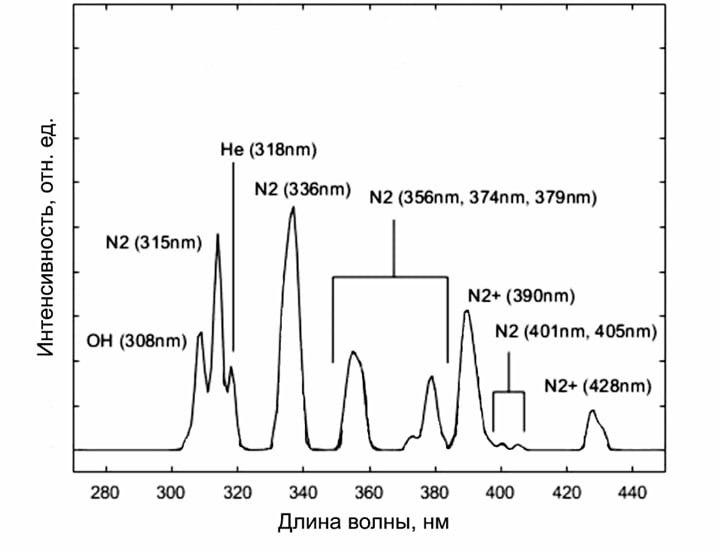
\includegraphics[width=\linewidth]{spec_ident_air.png}
    \caption{гелий с примесью воздуха, 300--440~нм~[3]}
  \end{subfigure}
  \caption{Опубликованные спектры для расшифровки наших: OH ---
  излучение осколков молекул воды, N$_2$ --- молекулы азота, N$_2^+$ ---
  ионы азота, He --- гелий.}
  \label{fig:ident}
\end{figure}

\begin{table}[H]
  \centering
  \caption{Что светится в наших спектрах.}
  \label{tab:lines}
  \begin{tabular}{ll}
    \toprule
    Длина волны, нм & Источник \\
    \midrule
    308--310 & пары воды (OH) \\
    315, 337, 357, 380 & азот, ультрафиолетовые полосы \\
    391, 428 & ионы азота \\
    580--780 (много полос) & азот, красные полосы \\
    389, 447, 471, 492, 502, 588, 668, 706, 728 & гелий \\
    777, 844 & кислород (видны и в эталоне [4]) \\
    \bottomrule
  \end{tabular}
\end{table}

\paragraph{Сравнение азота и гелия.}
Сравниваем самую яркую полосу азота 337~нм с линией гелия 501,6~нм:
обе регистрирует линейка Master, и на них не накладываются другие
полосы. Высоты пиков, прочитанные с графиков:
\begin{table}[H]
  \centering
  \caption{Высоты пиков азота и гелия на линейке Master (отсчёты) и их
  отношение.}
  \label{tab:ratio}
  \begin{tabular}{lcccc}
    \toprule
    Газ & $P_m$, Торр & $I_{337}$ (азот) & $I_{502}$ (гелий) &
    $I_{337}/I_{502}$ \\
    \midrule
    He чистый & 1   & 1450 & 5700 & 0,25 \\
    He чистый & 2,5 & 350  & 1500 & 0,23 \\
    He чистый & 5   & 2800 & $\approx 250$ & $\approx 11$ \\
    \midrule
    He техн.  & 1   & 2750 & 4300 & 0,64 \\
    He техн.  & 2,5 & 700  & 580  & 1,2 \\
    He техн.  & 5   & 6300 & $\lesssim 500$ (на уровне фона) & $\gtrsim 13$ \\
    \bottomrule
  \end{tabular}
\end{table}

Наблюдения:
\begin{itemize}
  \item при 1 и 2,5~Торр в чистом He спектр определяется гелием, самая
        яркая линия --- 667,8~нм;
  \item в техническом He азота при каждом давлении больше, чем в
        чистом: отношение $I_{337}/I_{502}$ в 2,5--5 раз выше. При
        2,5~Торр азот и гелий уже сравнимы ($\approx 1{,}2$);
  \item между 2,5 и 5~Торр отношение в обоих газах вырастает в 10--50
        раз. При 5~Торр линии гелия на Master почти не видны, а на Slave
        вместо отдельных линий гелия --- гребёнка красных полос азота;
  \item в чистом He при 5~Торр самый яркий пик спектра --- полоса паров
        воды 309~нм; при 1--2,5~Торр она слабая.
\end{itemize}
Отсюда давление, при котором азот начинает преобладать:
$P^* \approx 2{,}5$~Торр (между 2,5 и 5) для технического He и
$2{,}5 < P^* < 5$~Торр для чистого. Точнее определить $P^*$ нельзя:
спектров между 2,5 и 5~Торр нет.

Важная оговорка: в том же интервале давлений (3,5--3,9~Торр) разряд
переходит из $\alpha$- в $\gamma$-форму. При этом меняются распределение
электронов по энергиям и нагрев газа, а значит, и то, какие состояния
возбуждаются. Поэтому резкий рост полос азота может быть связан не
только с передачей возбуждения от гелия, но и со сменой формы разряда.

\paragraph{Методика проверки оптической прозрачности.}
Для каждого давления снимаются спектры: только лампы $S_\text{л}$, только
разряда $S_\text{р}$ и разряда с включённой лампой $S_\text{р+л}$. Если
плазма оптически тонкая, то $S_\text{р+л} = S_\text{р} + S_\text{л}$ в
пределах шума, и в $S_\text{р+л} - S_\text{л}$ нет провалов (линий
поглощения) на длинах волн линий плазмы.

\begin{figure}[H]
  \centering
  \begin{subfigure}{0.7\linewidth}
    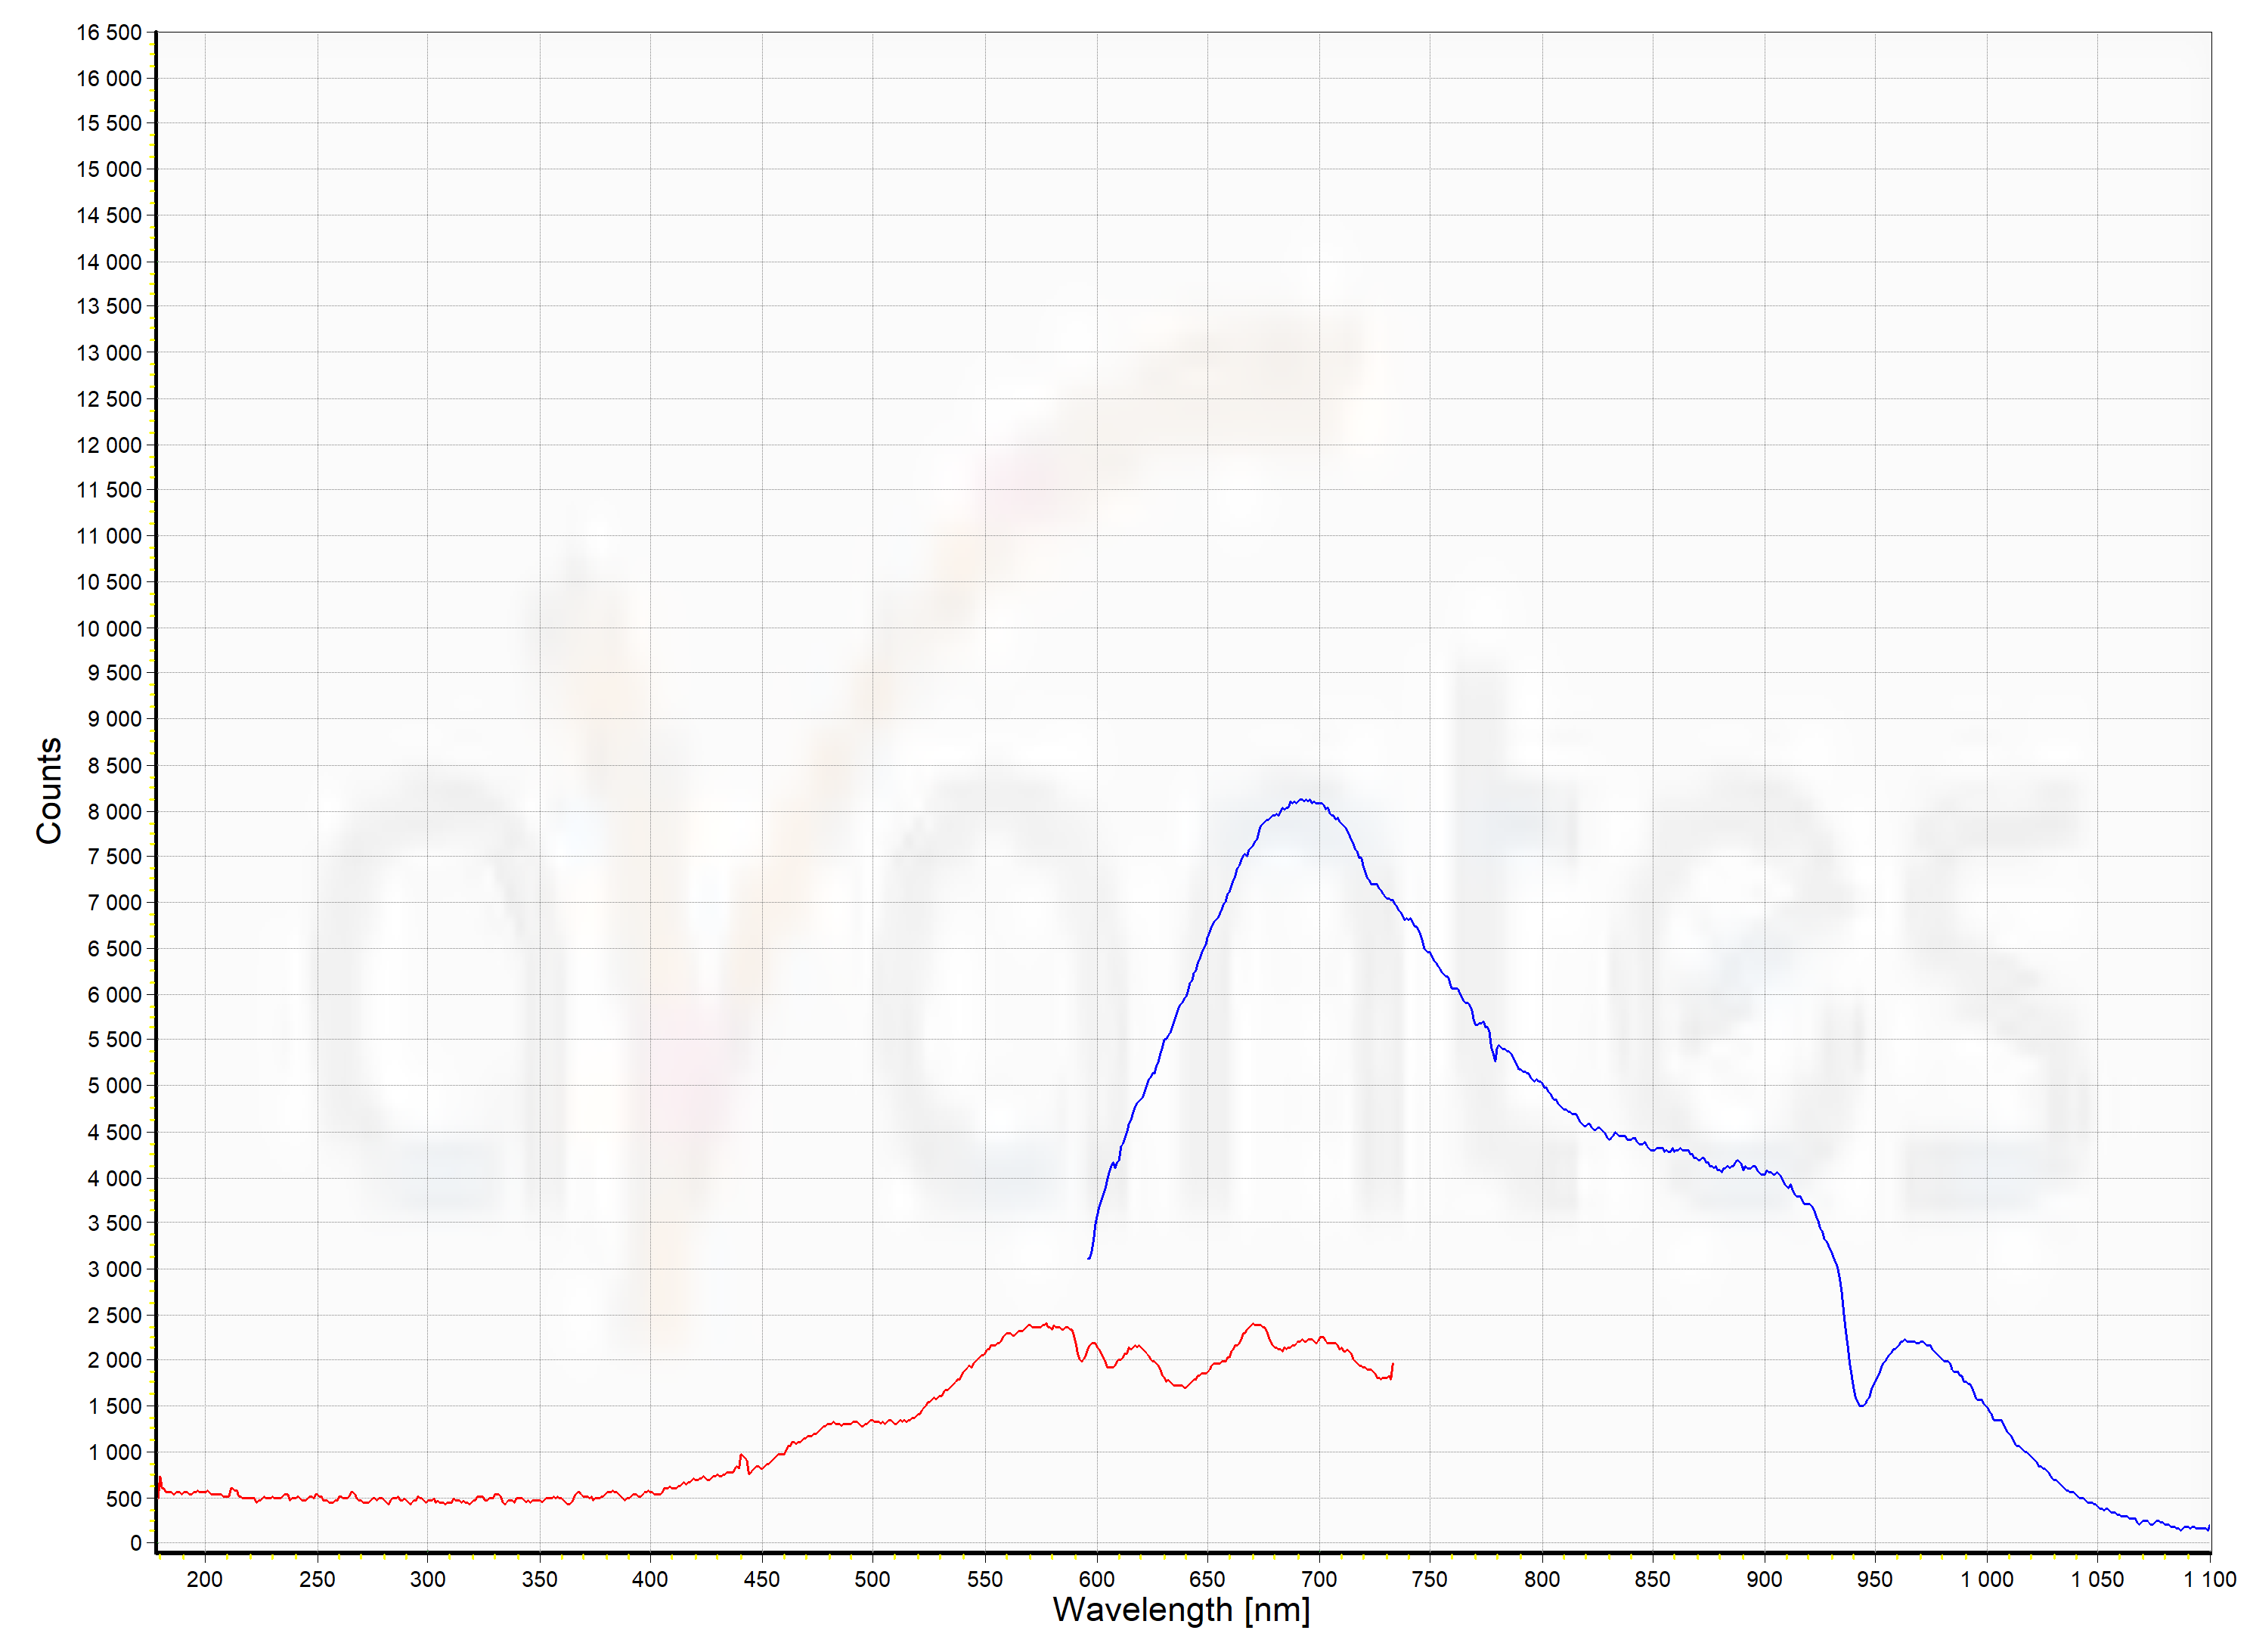
\includegraphics[width=\linewidth]{spec_lamp_2500ms.png}
    \caption{2,5~с}
  \end{subfigure}\\[4pt]
  \begin{subfigure}{0.49\linewidth}
    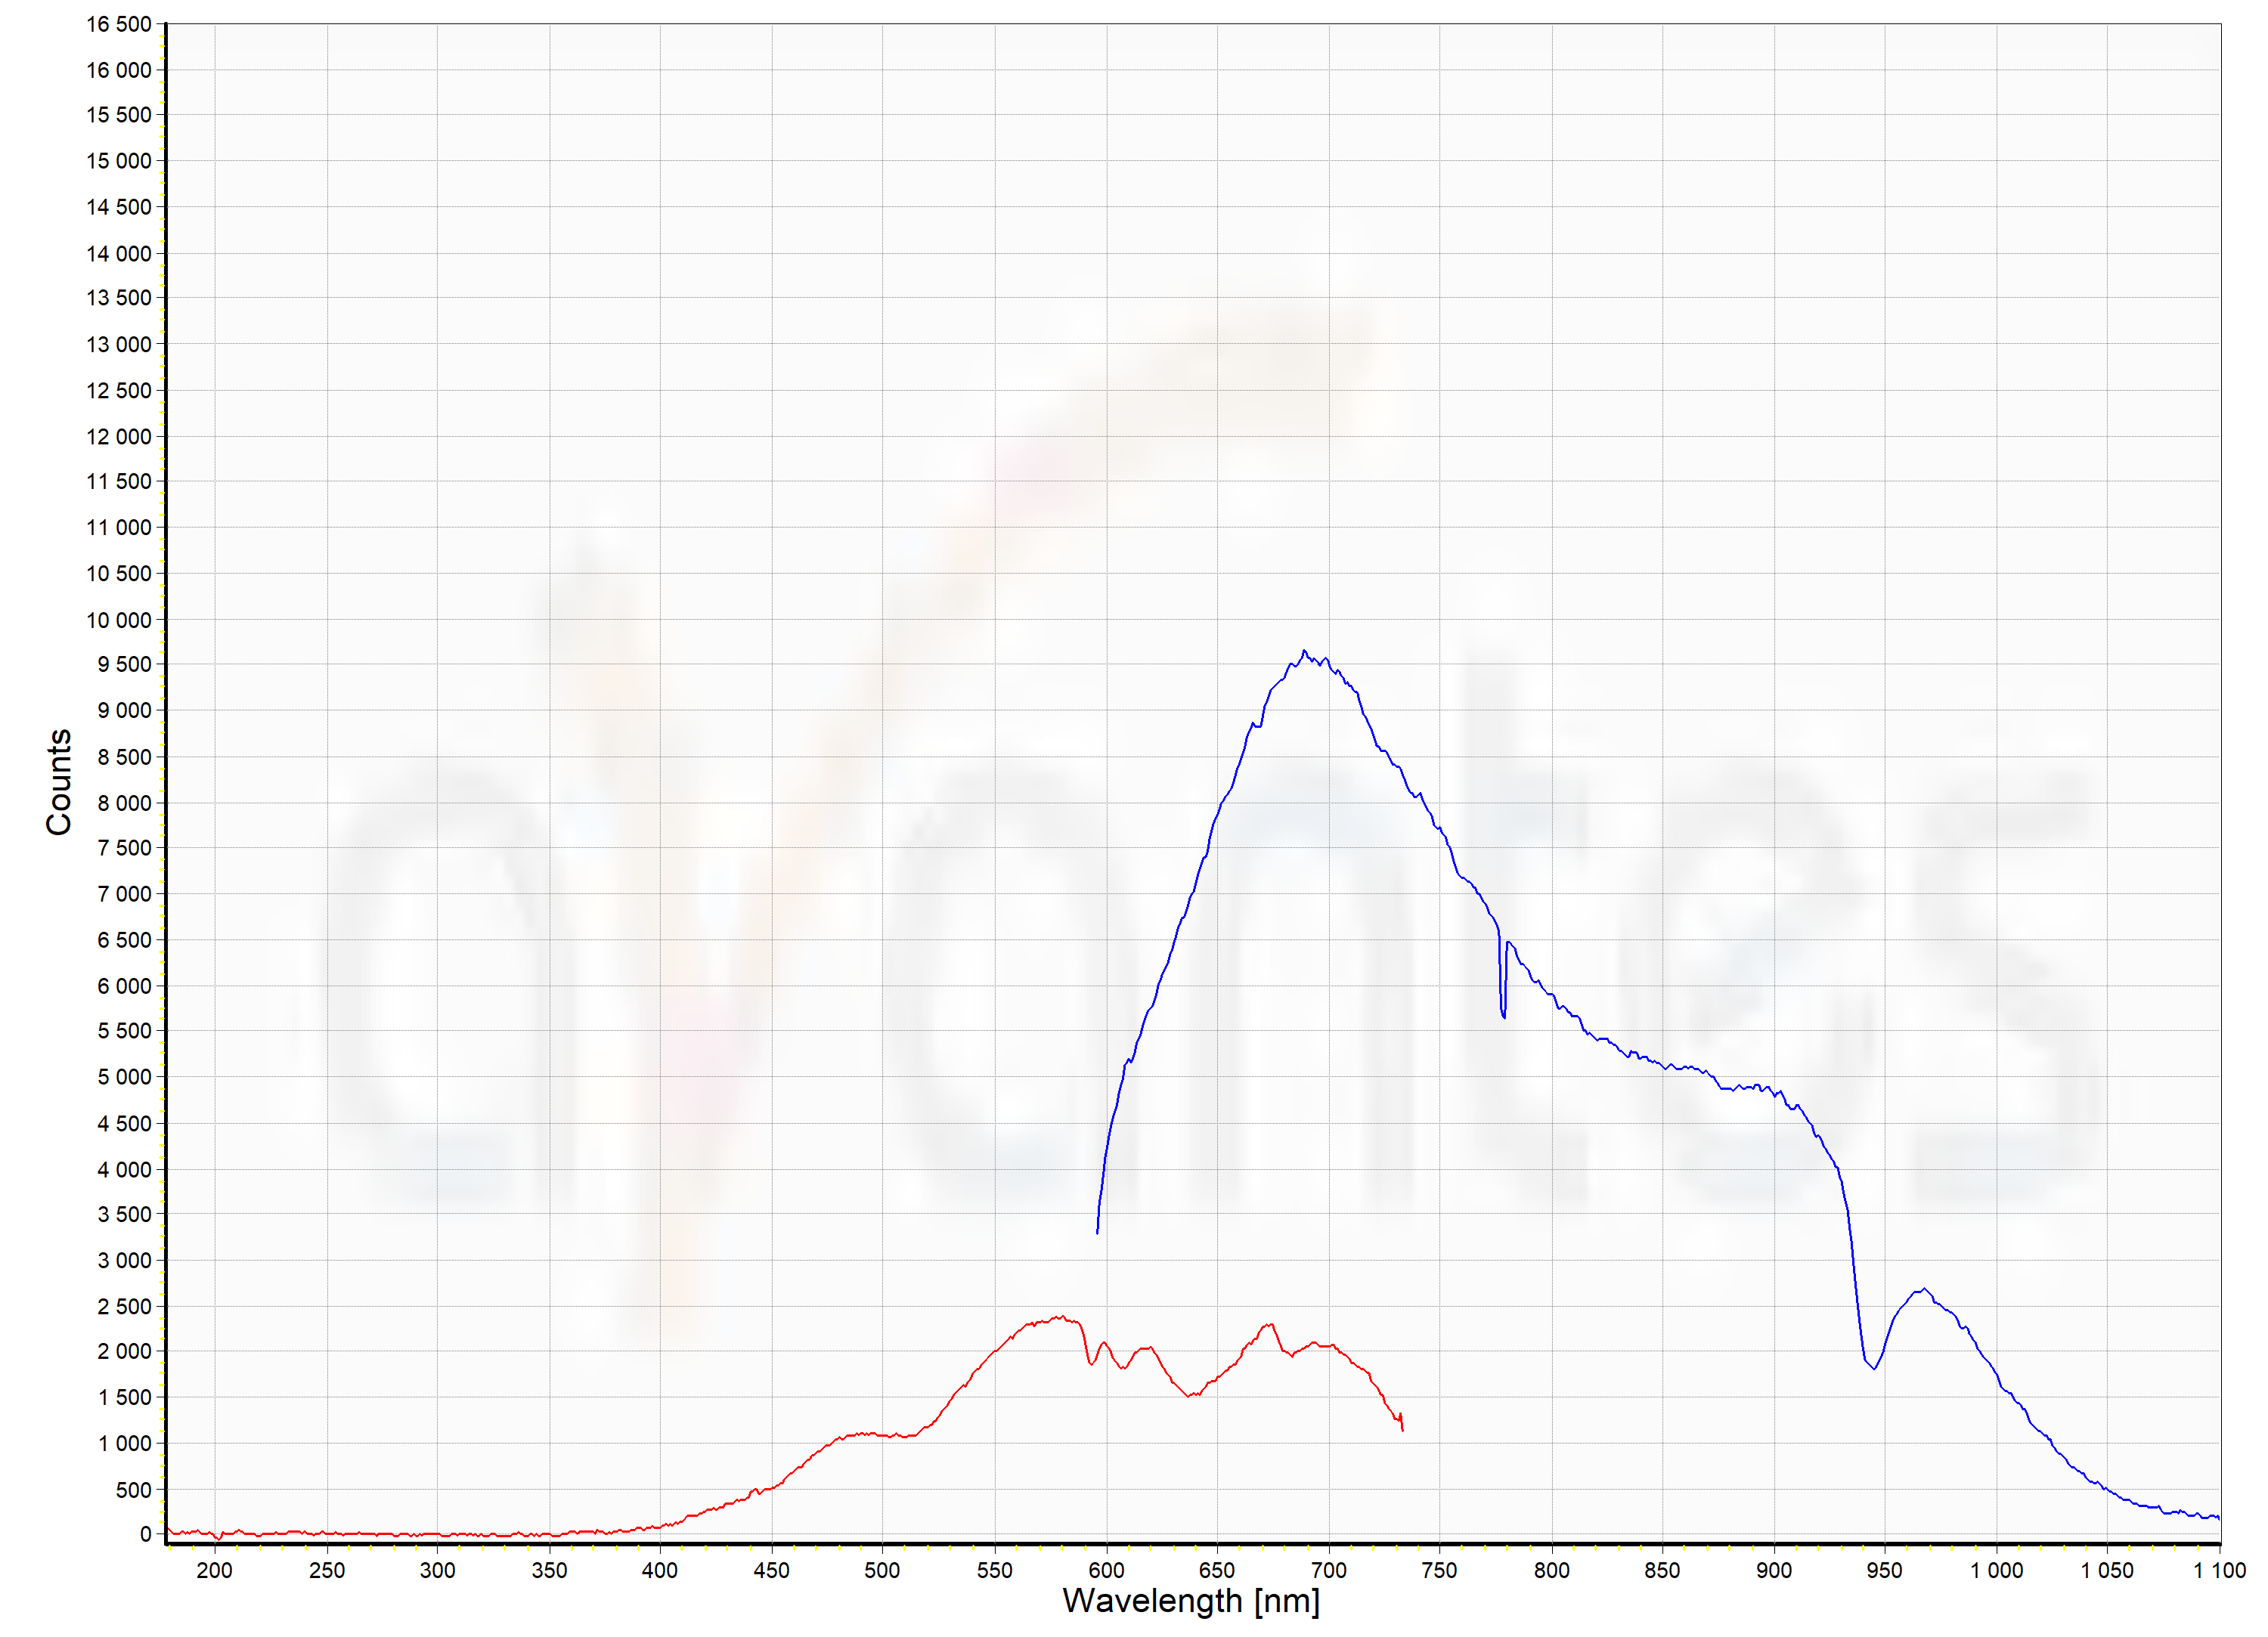
\includegraphics[width=\linewidth]{spec_lamp_3000ms.png}
    \caption{3~с}
  \end{subfigure}\hfill
  \begin{subfigure}{0.49\linewidth}
    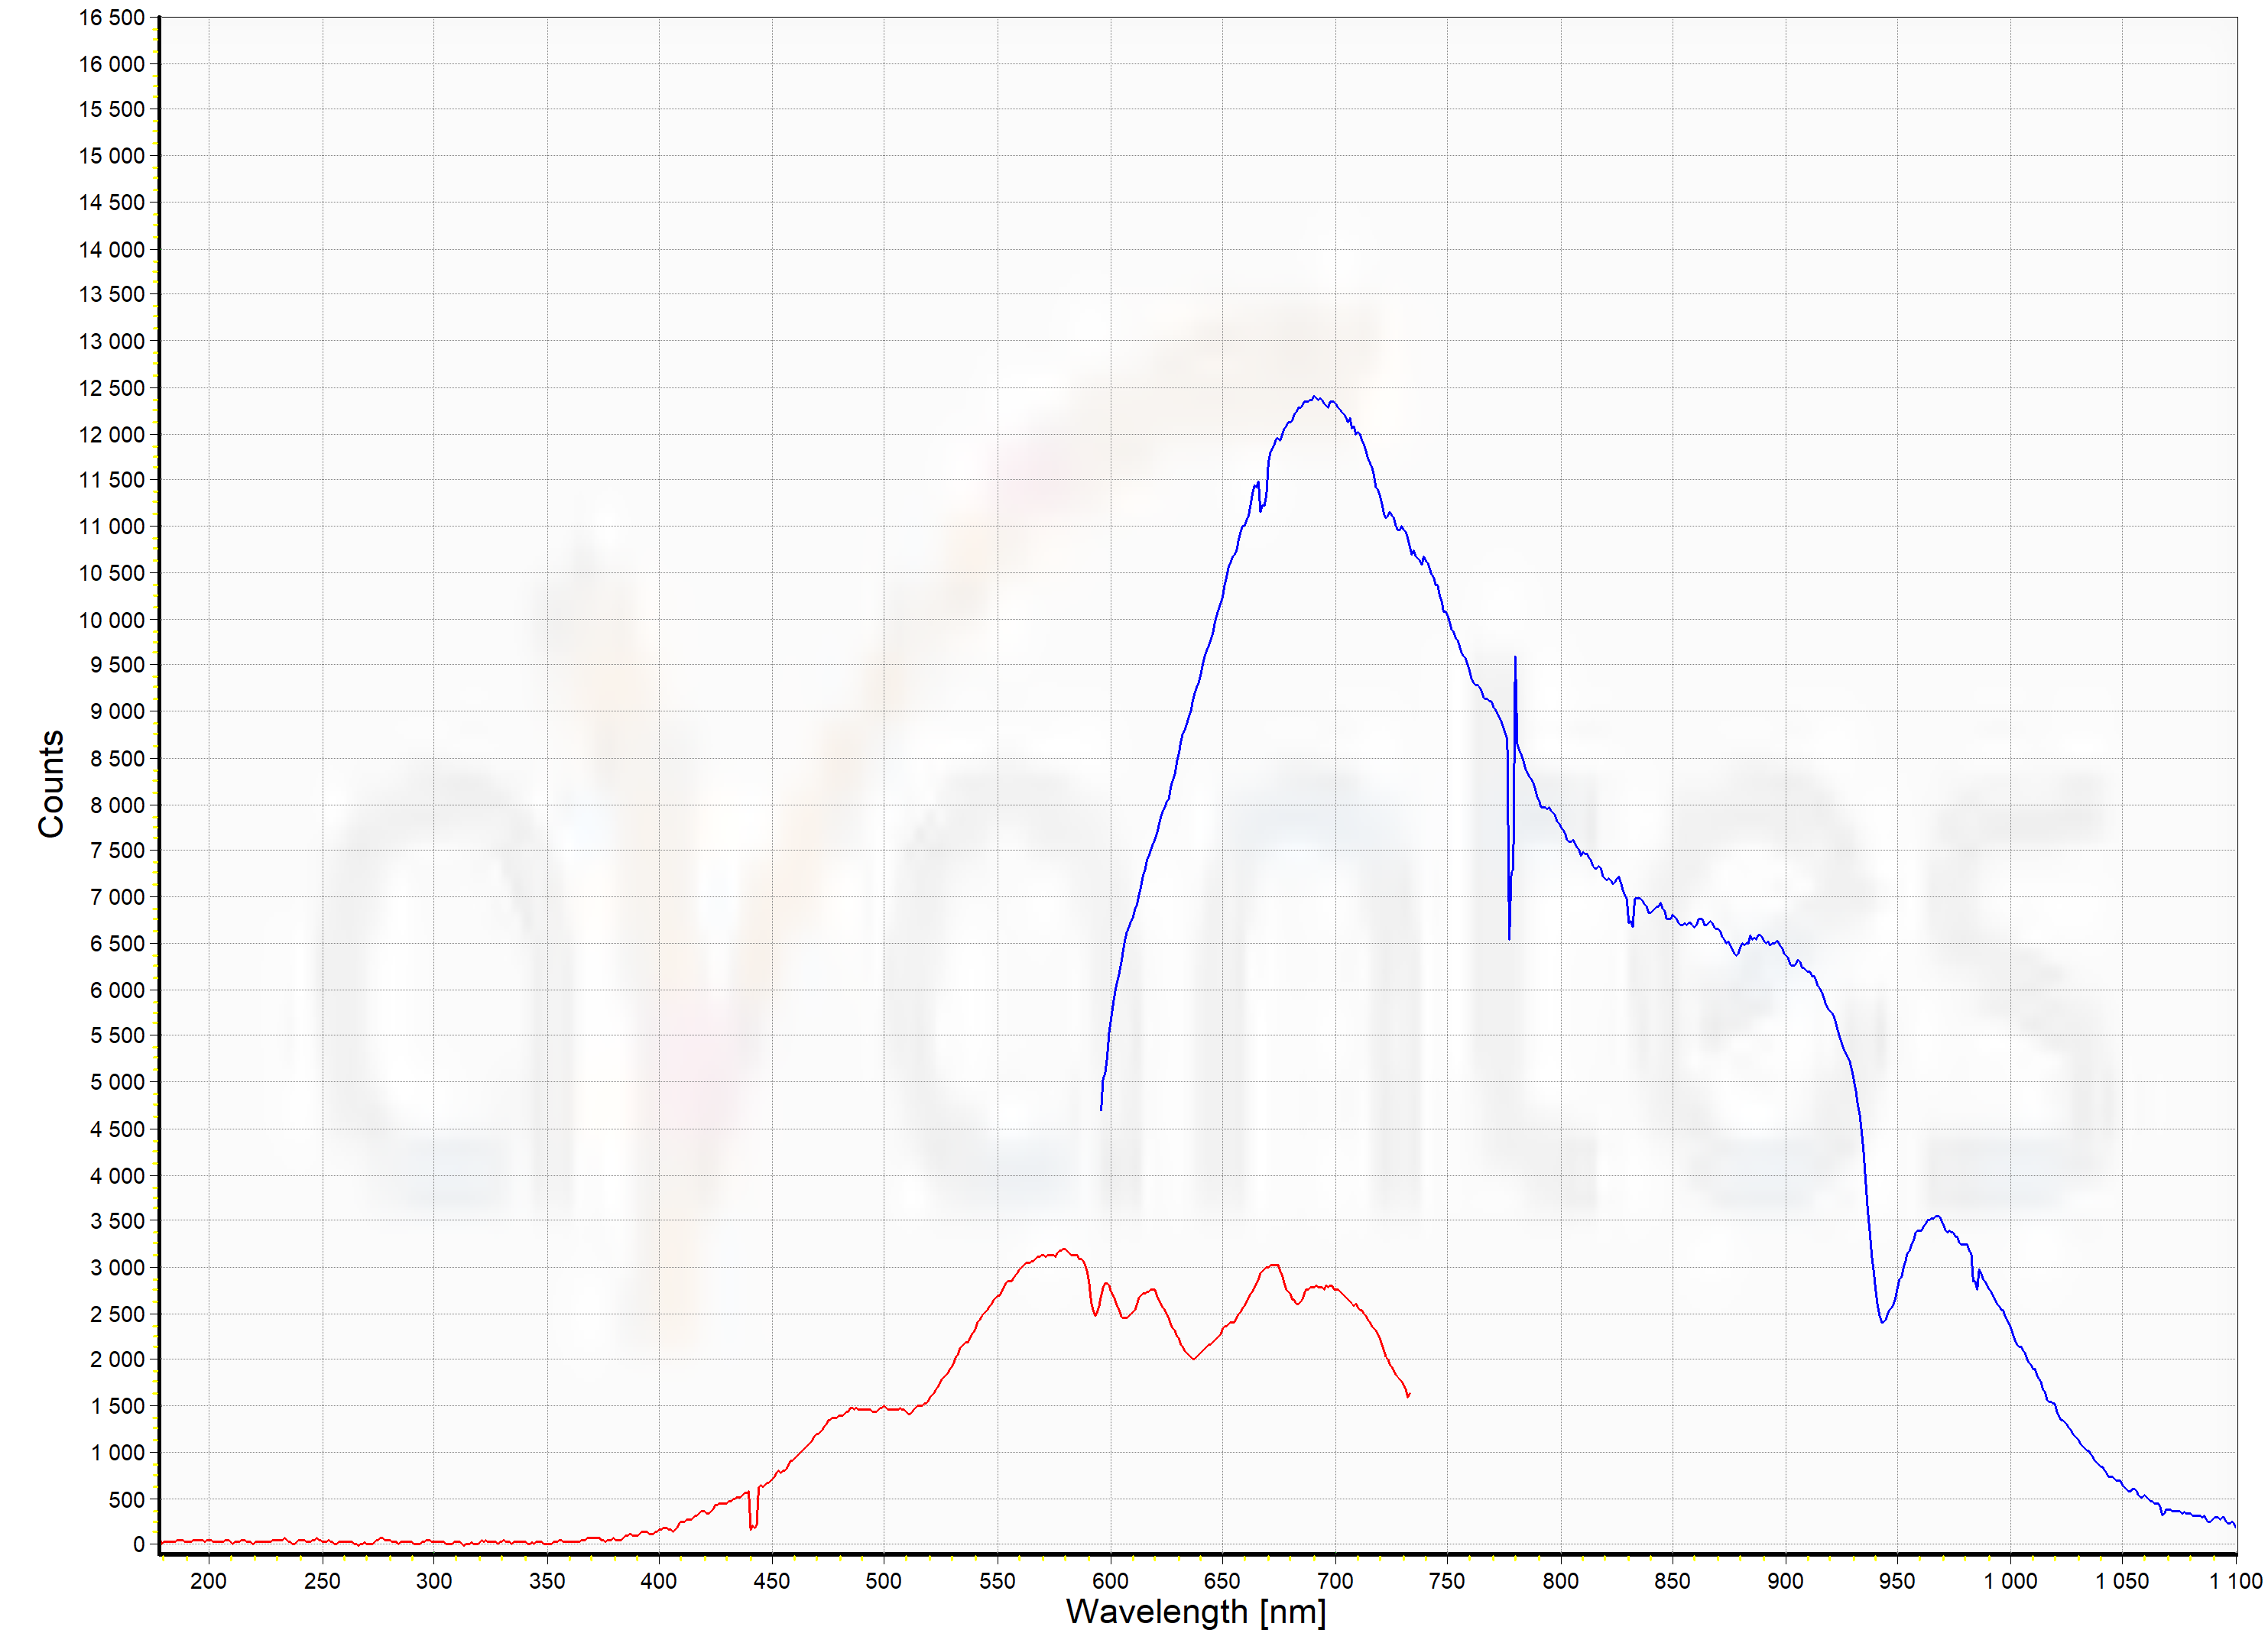
\includegraphics[width=\linewidth]{spec_lamp_4000ms.png}
    \caption{4~с}
  \end{subfigure}
  \caption{Спектр эталонной галогенной лампы $S_\text{л}$ при временах
  накопления, использованных для спектров разряда. Спектр непрерывный,
  без линий. Провал у 940~нм есть и без плазмы, то есть это свойство
  лампы и спектрометра, а не поглощение в разряде.}
  \label{fig:lamp}
\end{figure}

\paragraph{Результат проверки прозрачности.}
Для четырёх режимов из спектра <<разряд + лампа>> вычтен спектр лампы
с тем же временем накопления. Результат $S_\text{р+л}-S_\text{л}$
сравнивается со спектром одного разряда $S_\text{р}$
(рис.~\ref{fig:transp}). Если плазма прозрачна, кривые должны совпасть.

\begin{figure}[H]
  \centering
  \begin{subfigure}{0.49\linewidth}
    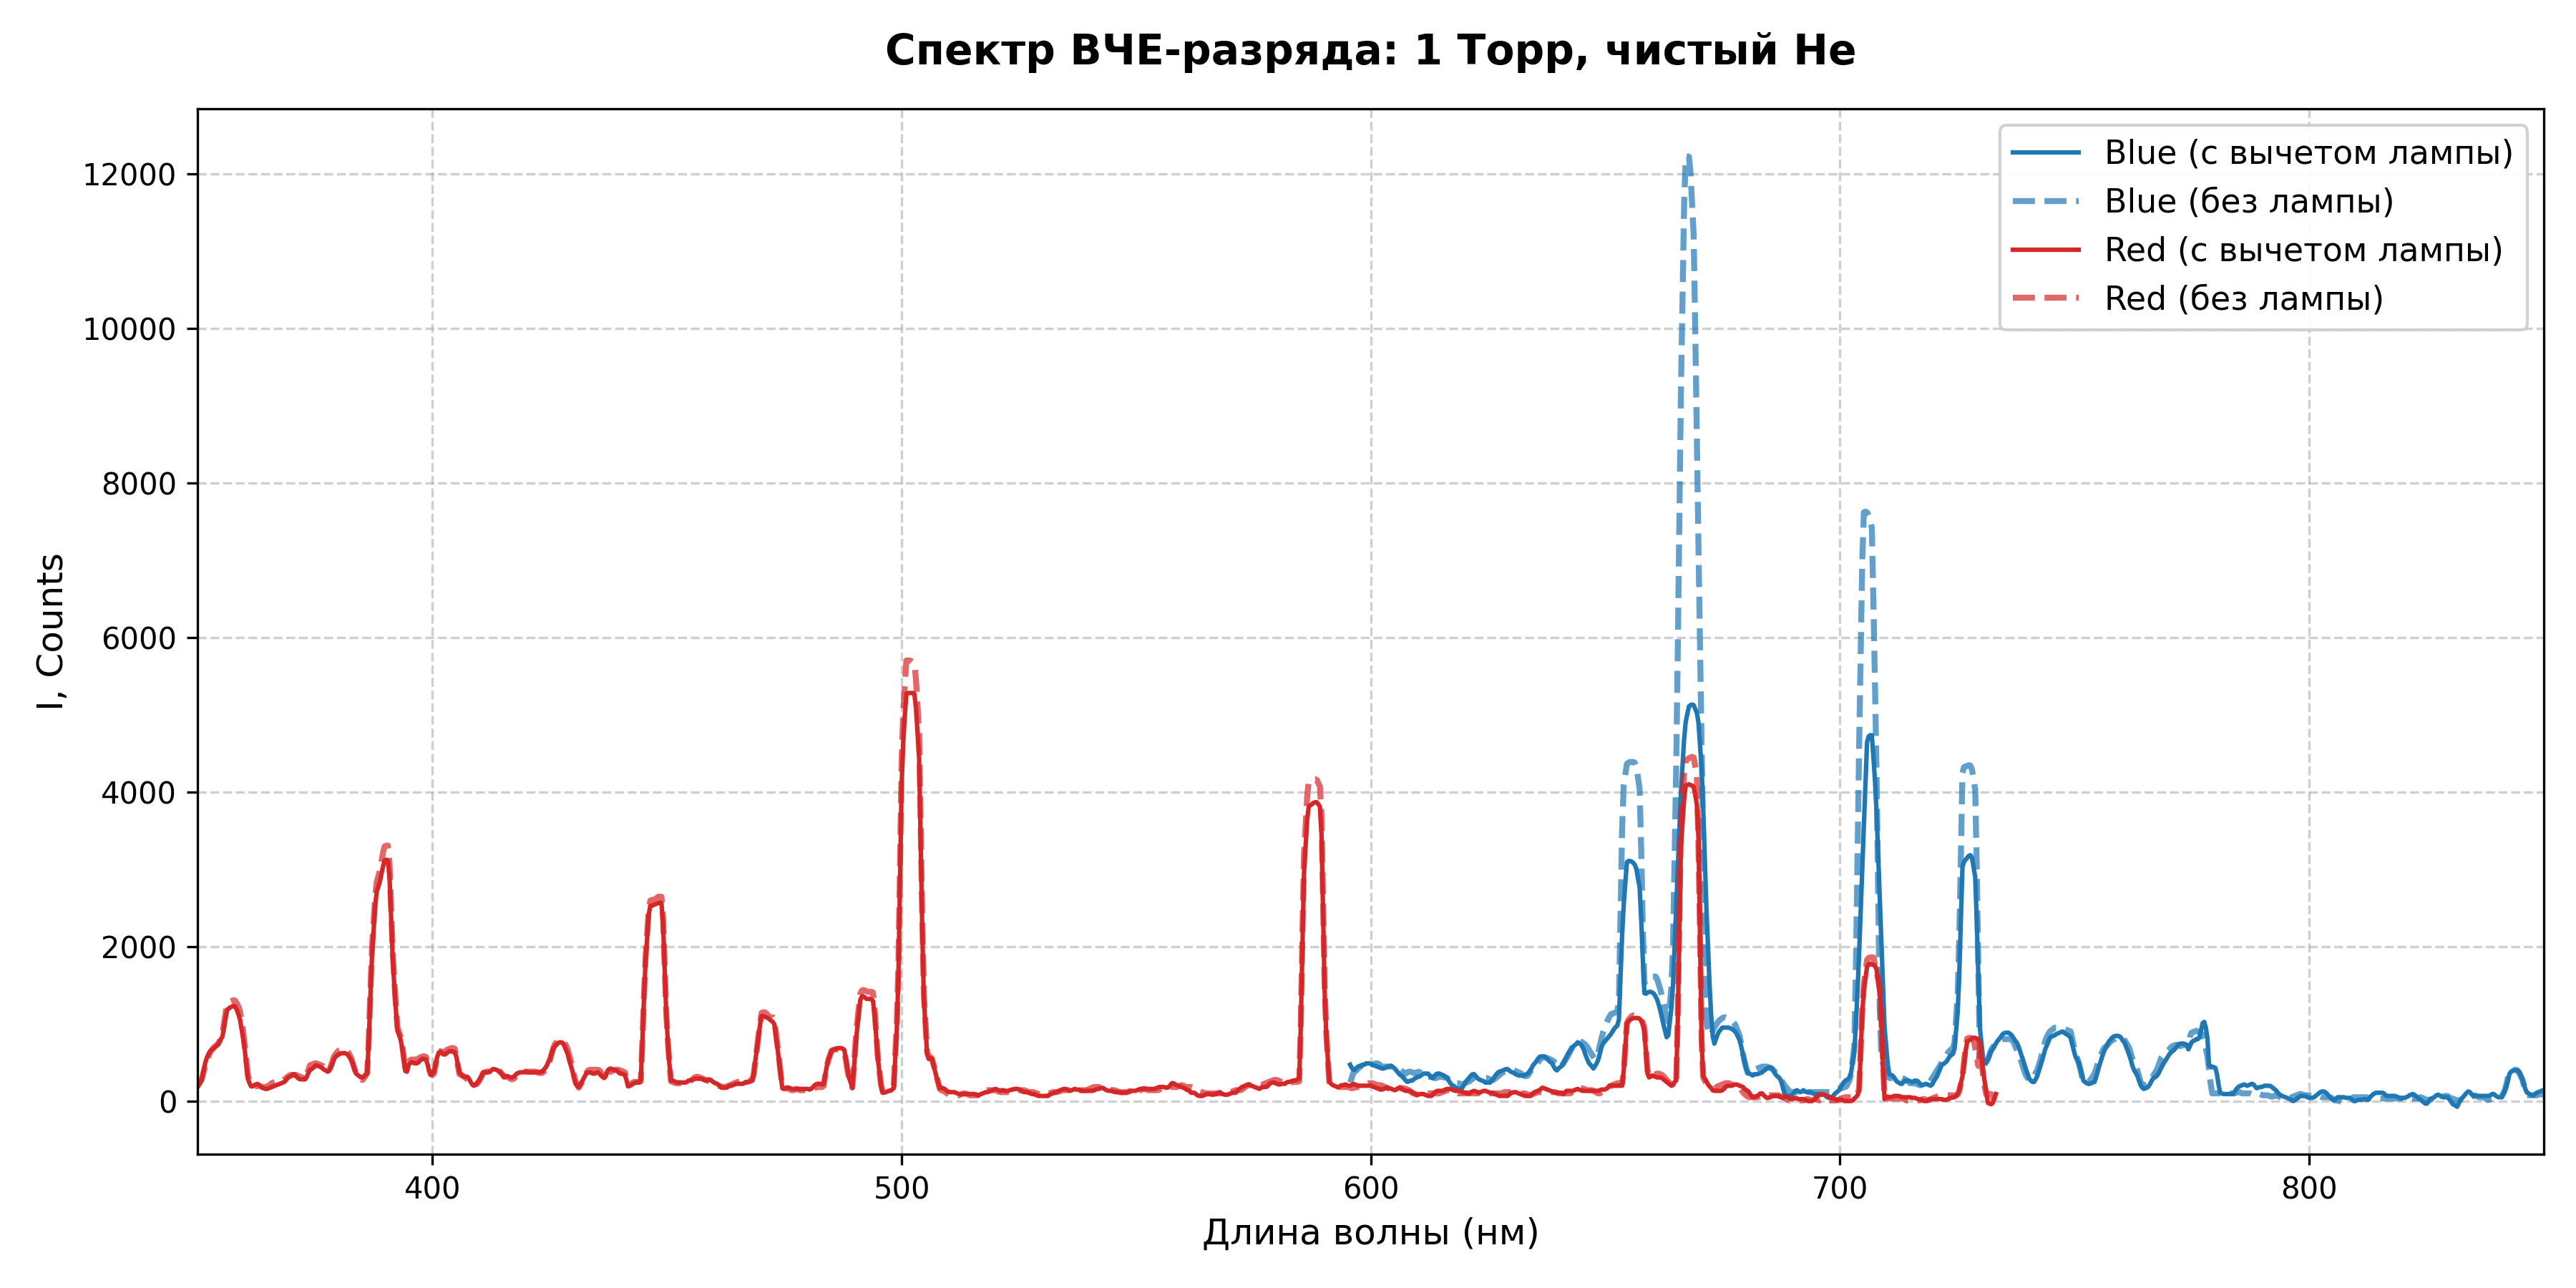
\includegraphics[width=\linewidth]{transp_He_1torr.png}
    \caption{чистый He, 1~Торр}
  \end{subfigure}\hfill
  \begin{subfigure}{0.49\linewidth}
    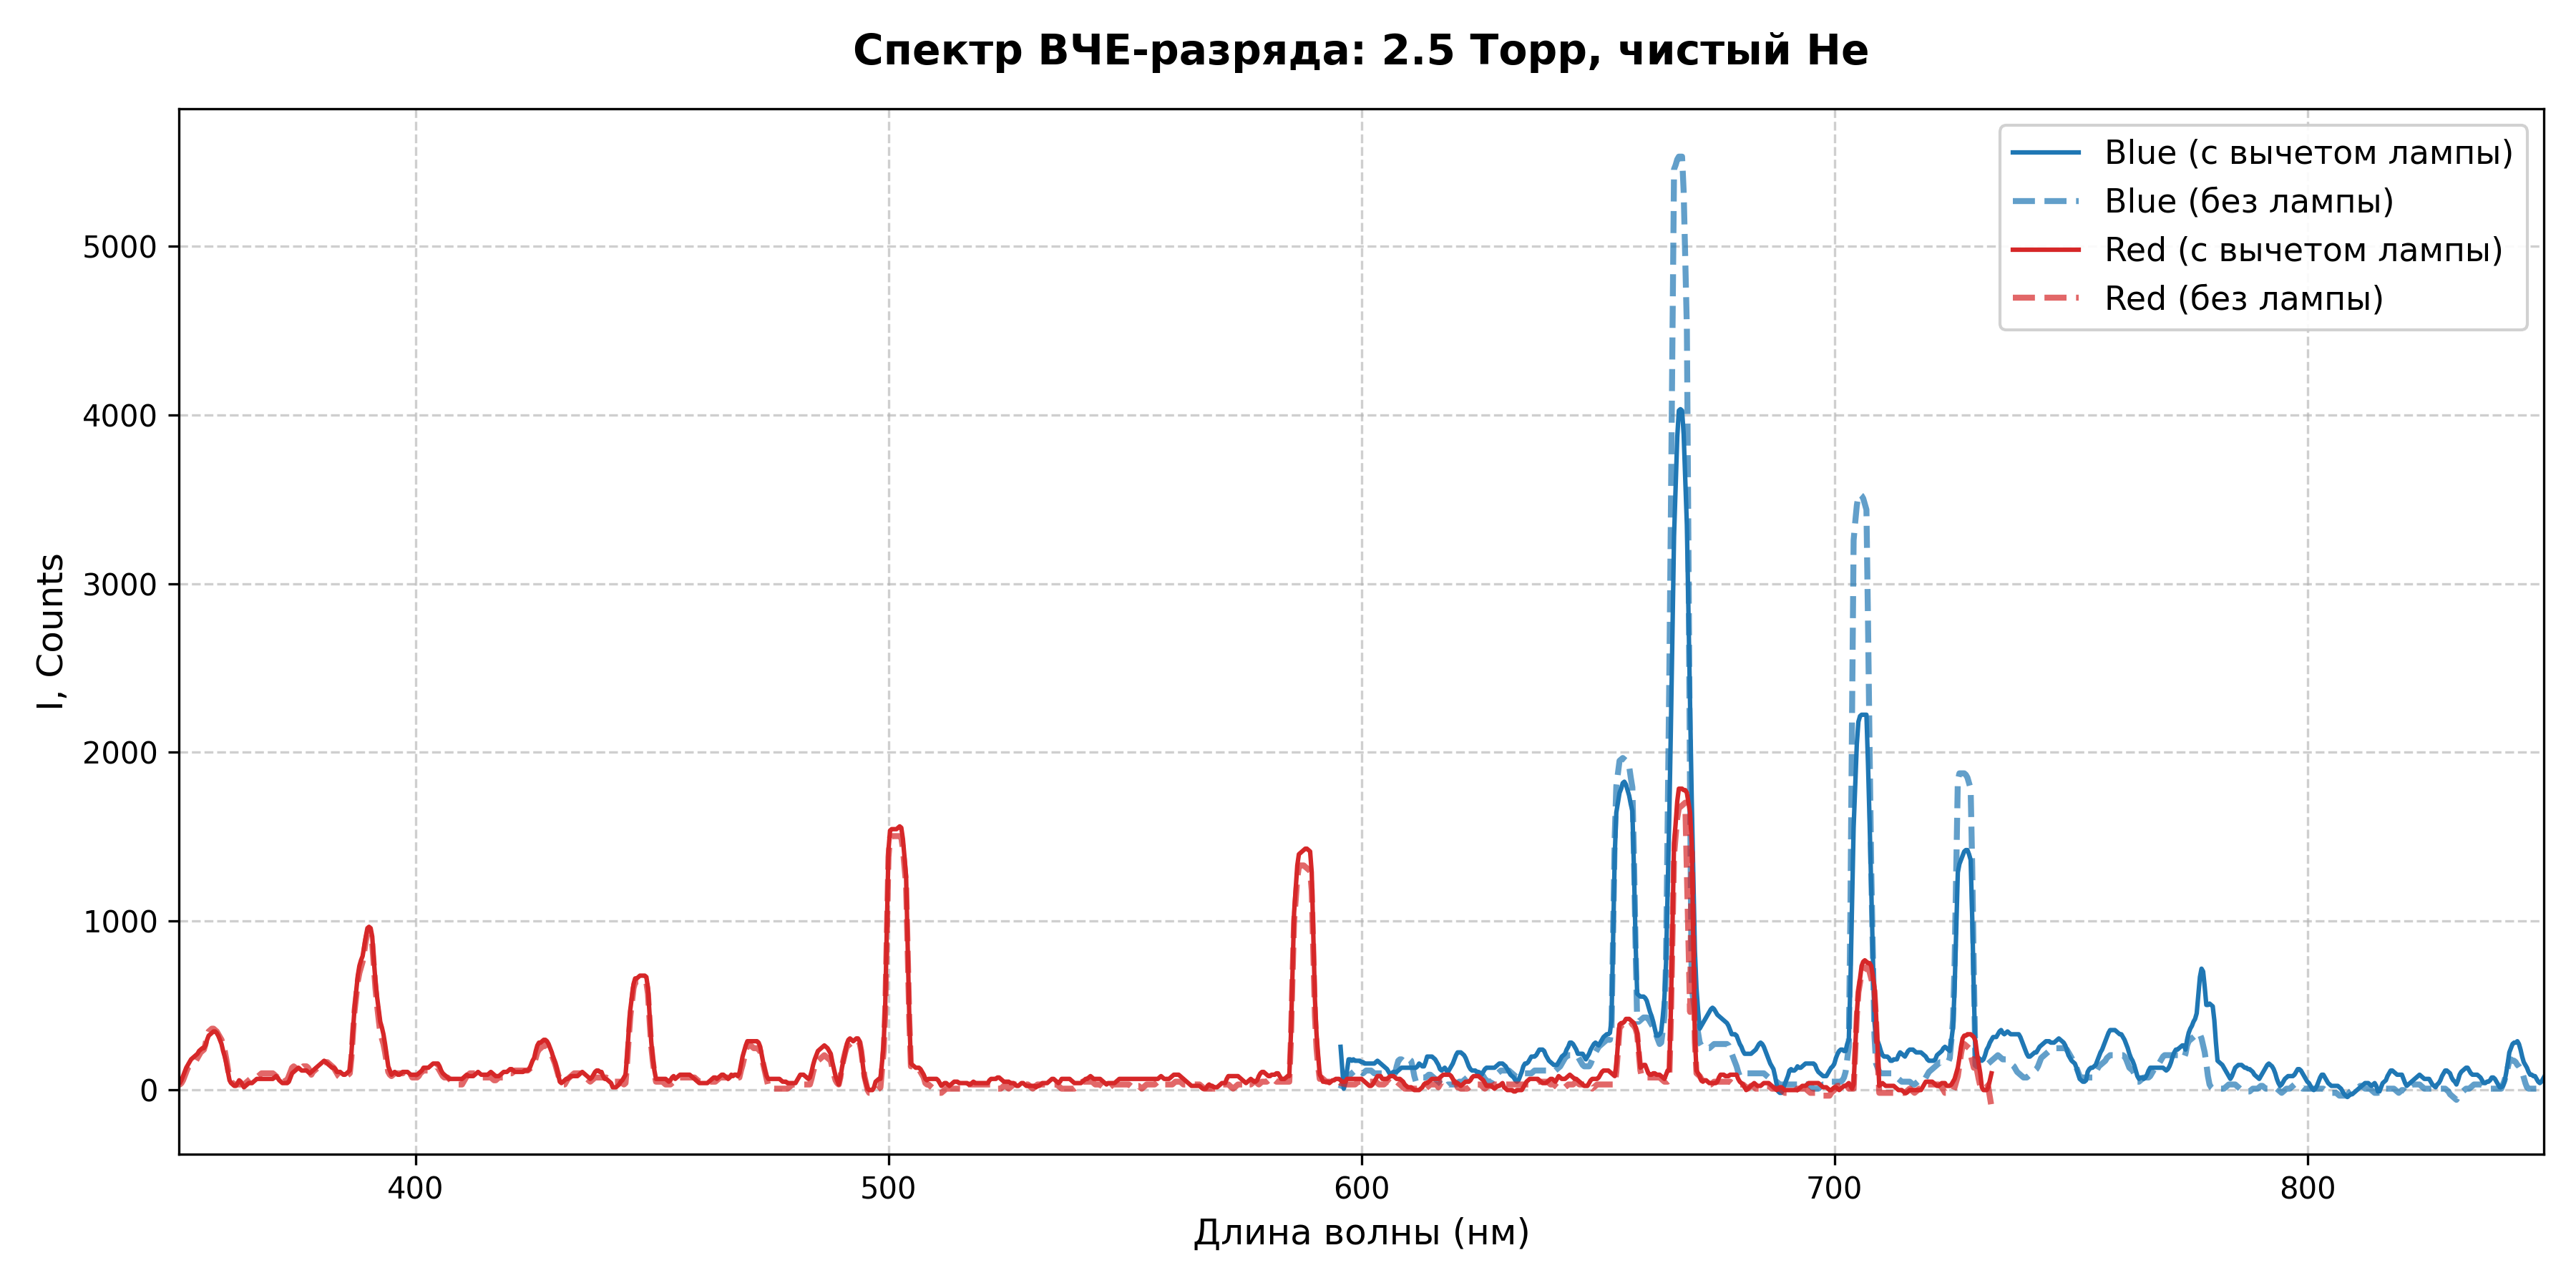
\includegraphics[width=\linewidth]{transp_He_2.5torr.png}
    \caption{чистый He, 2,5~Торр}
  \end{subfigure}\\[4pt]
  \begin{subfigure}{0.49\linewidth}
    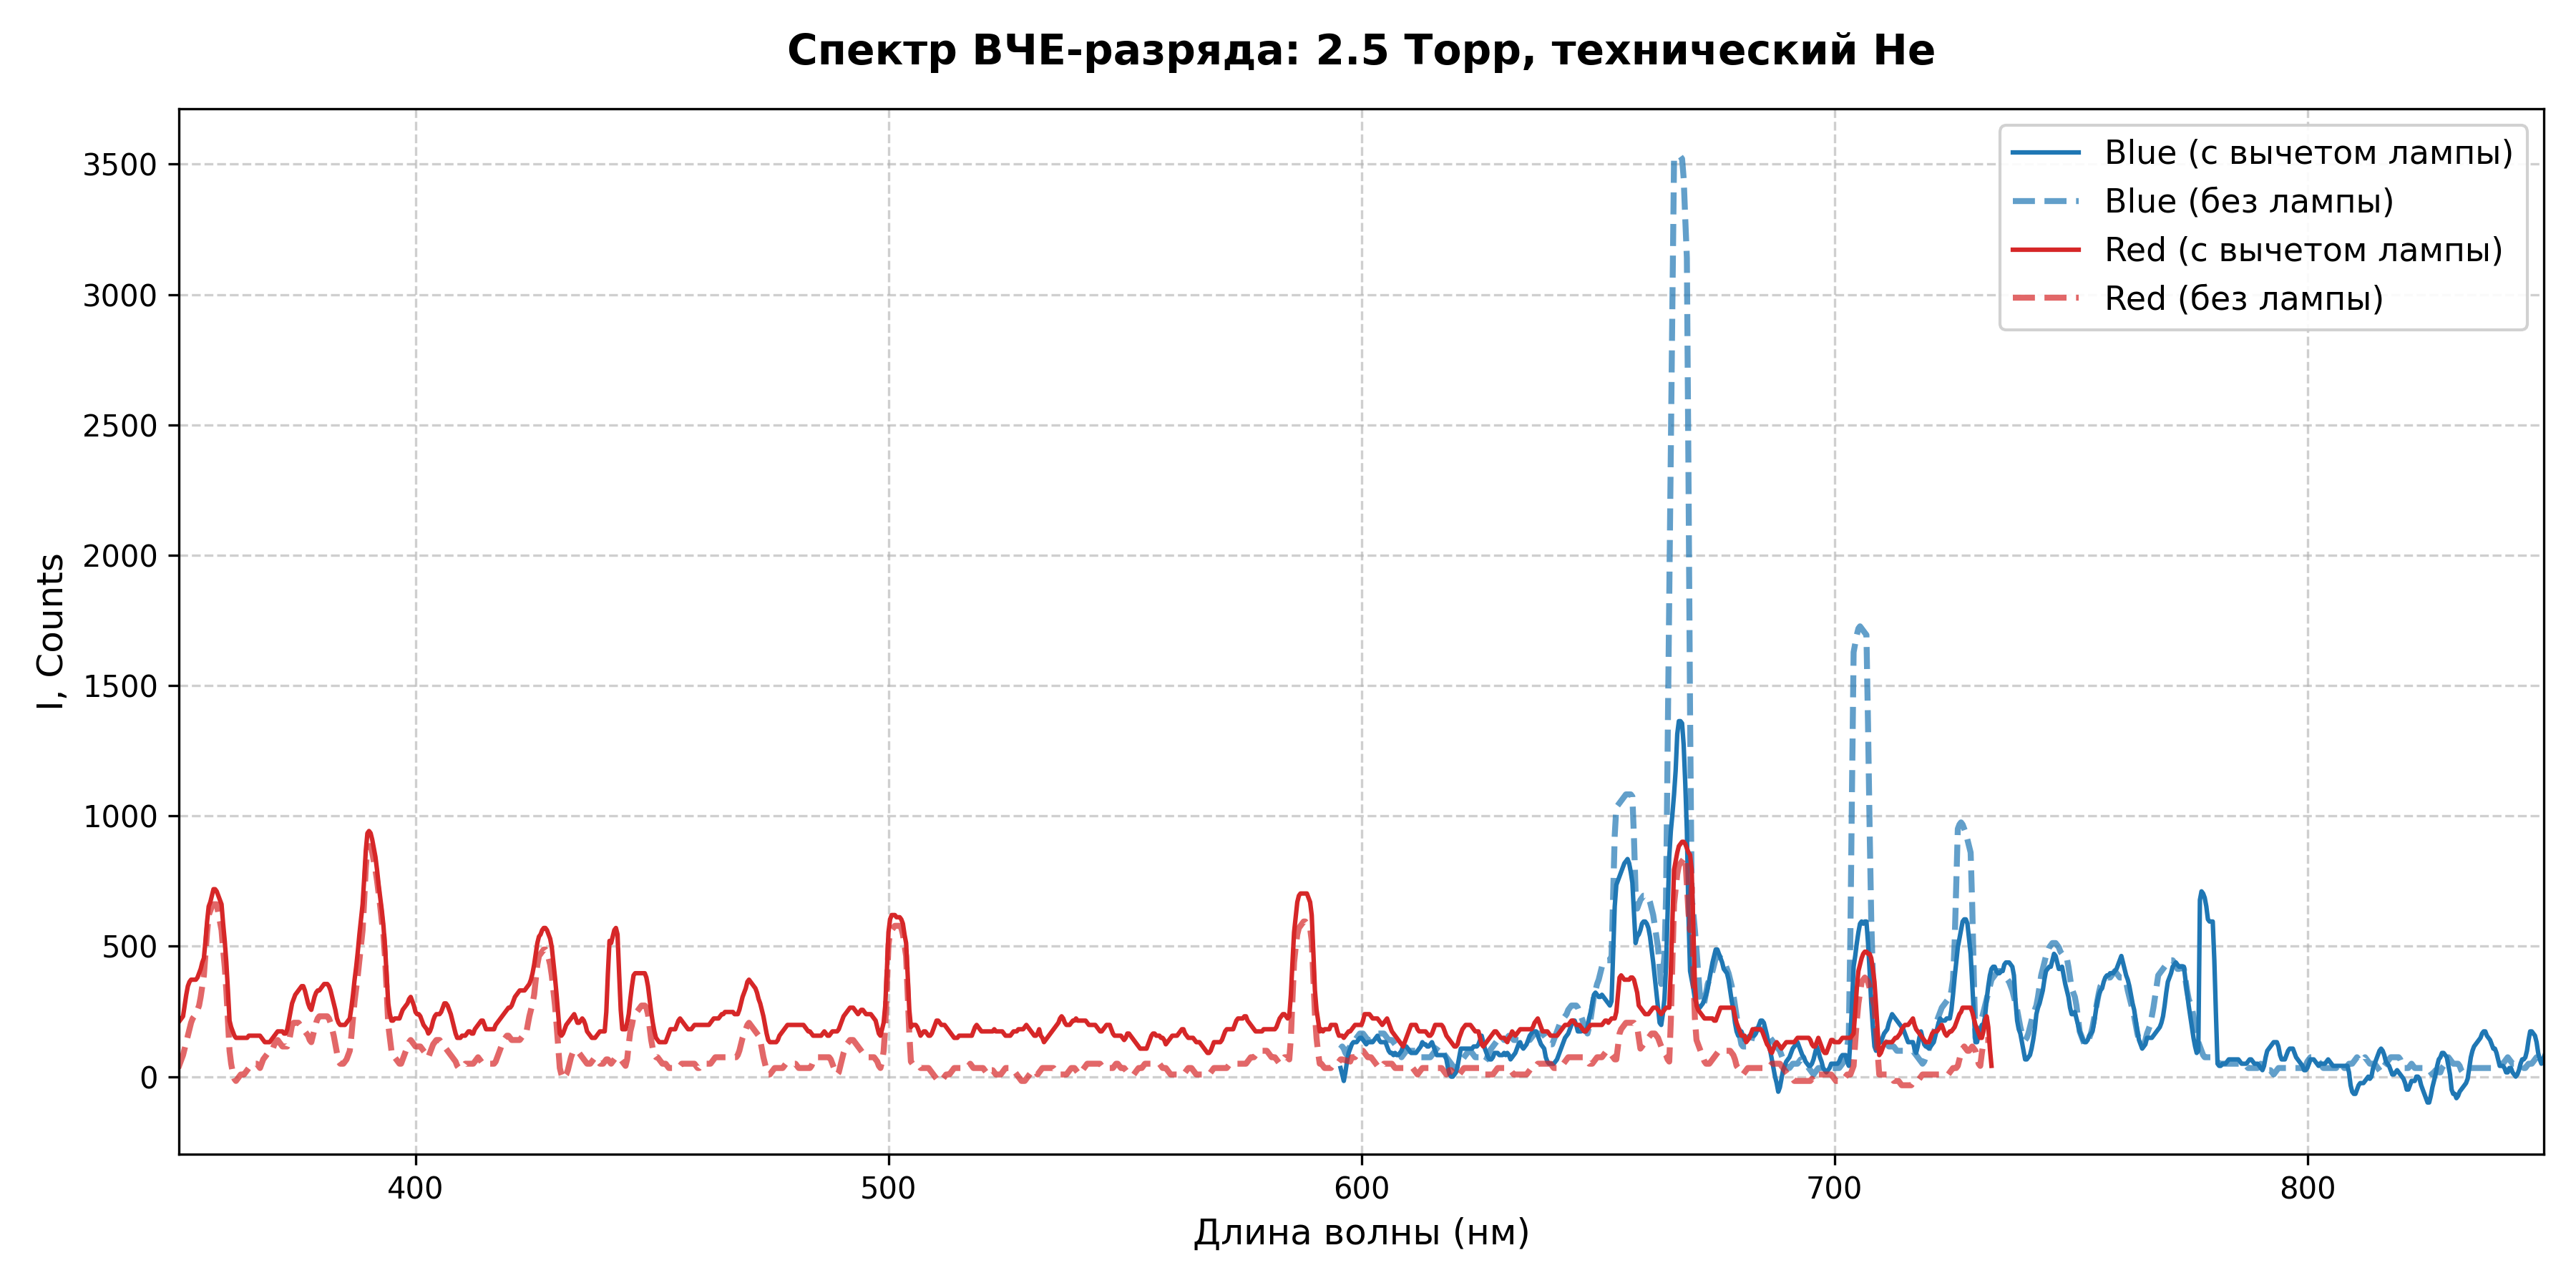
\includegraphics[width=\linewidth]{transp_He_tech_2.5torr.png}
    \caption{технический He, 2,5~Торр}
  \end{subfigure}\hfill
  \begin{subfigure}{0.49\linewidth}
    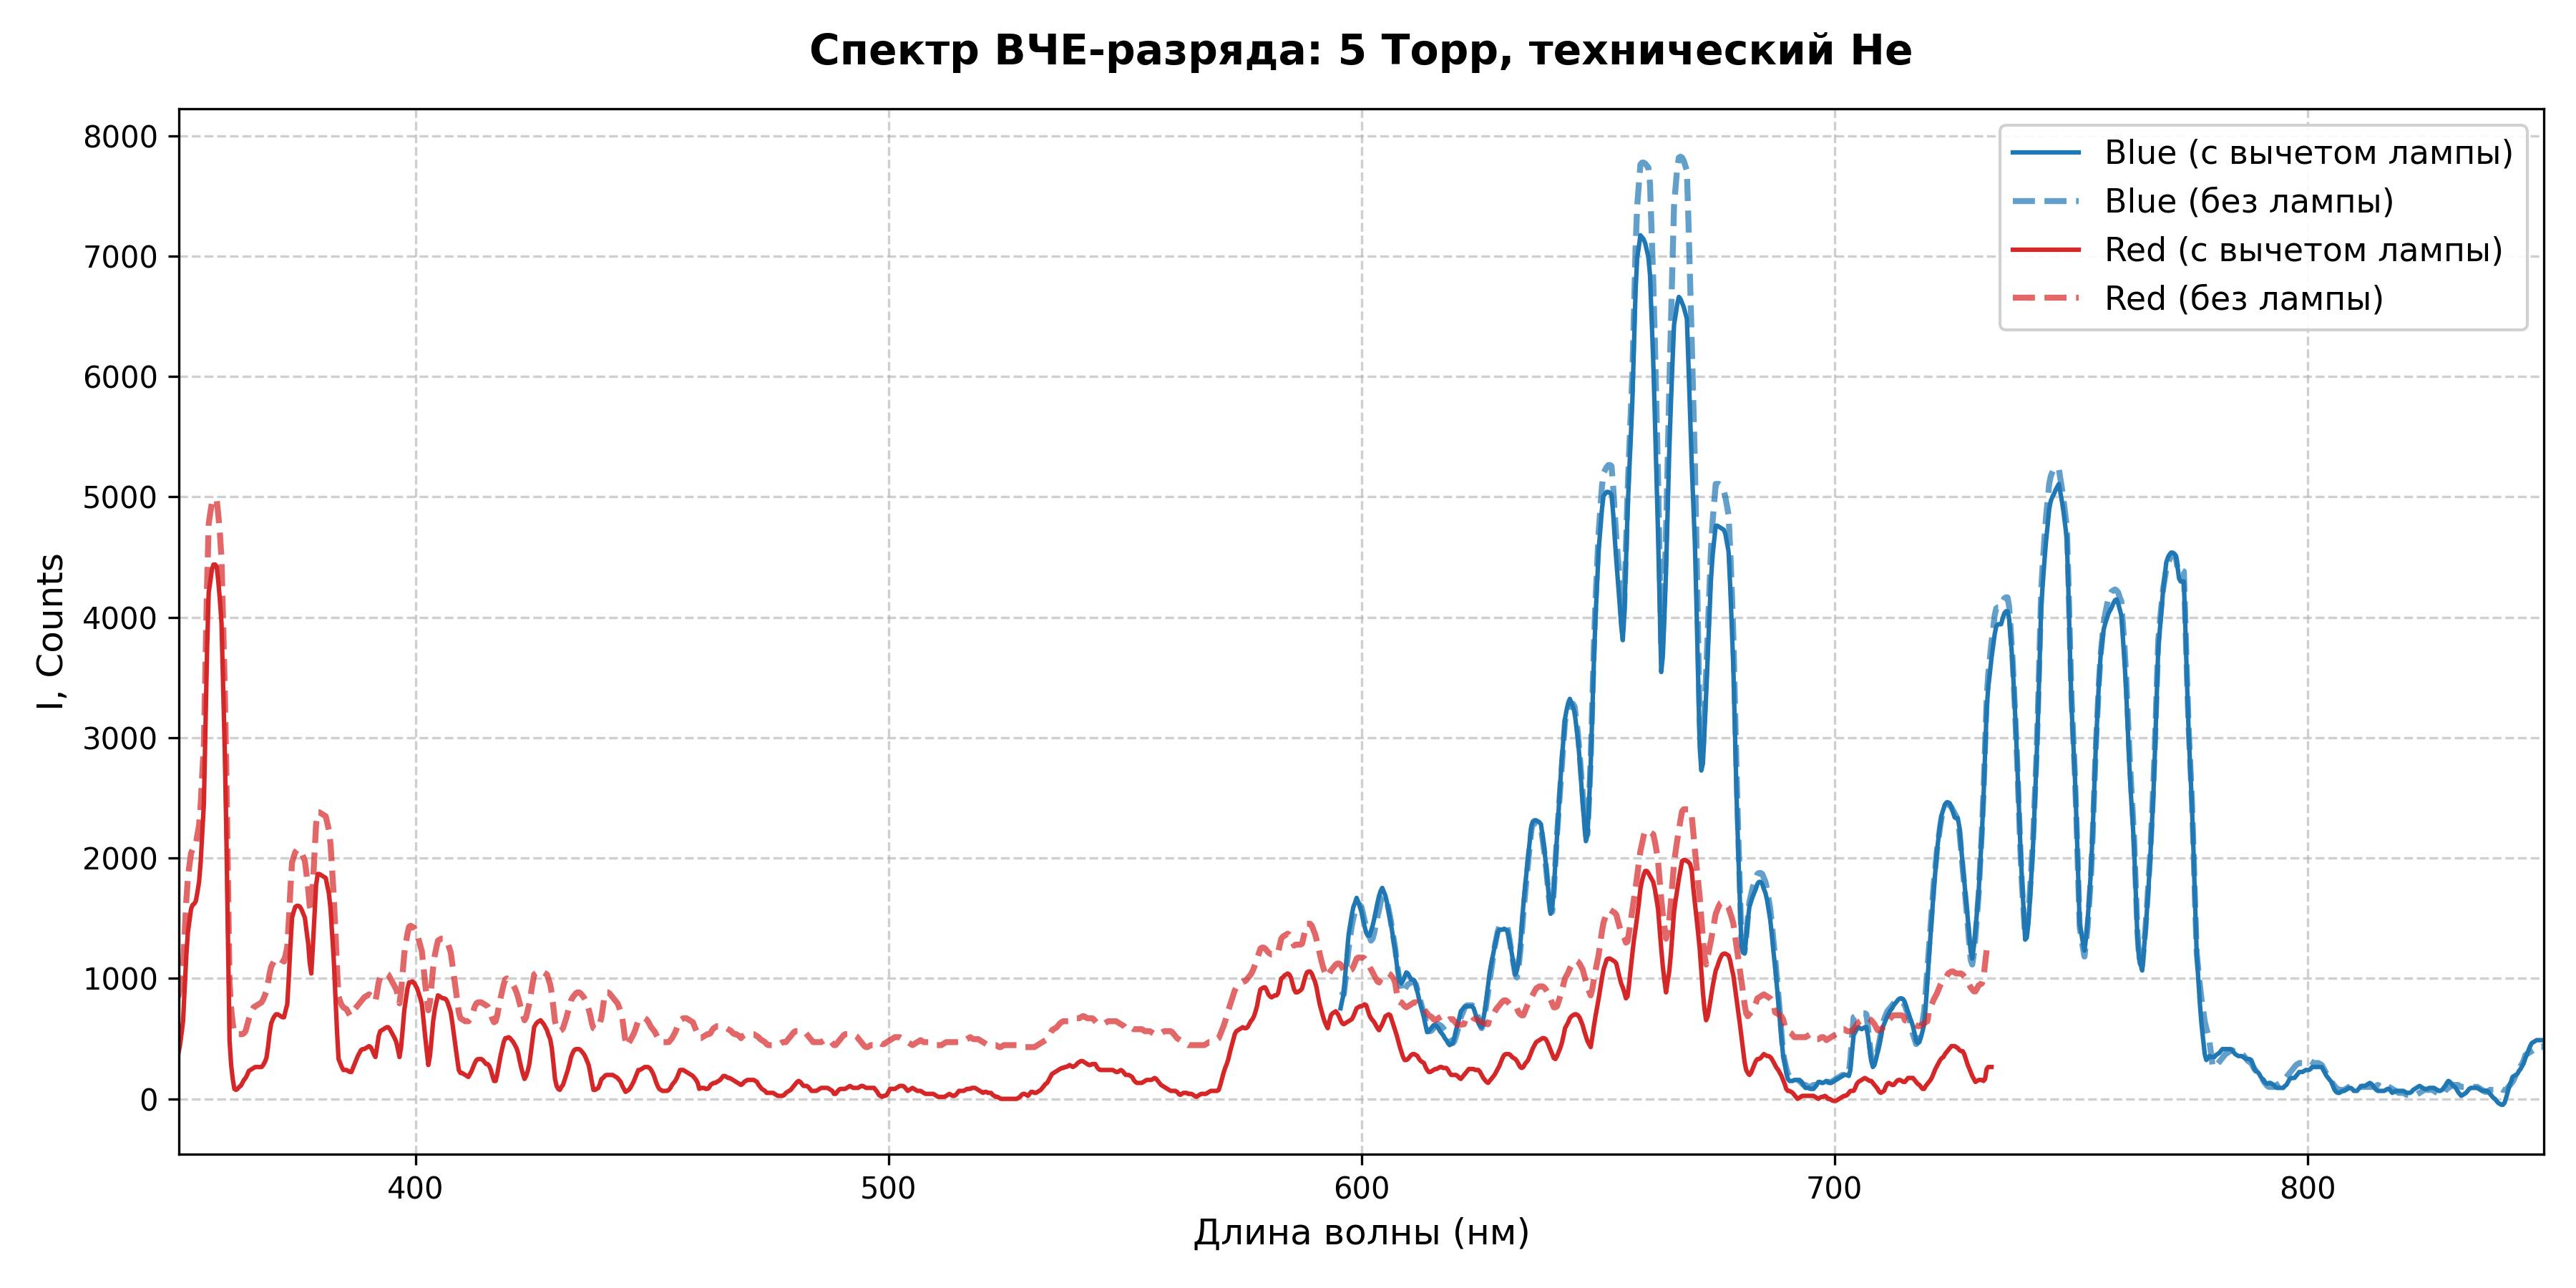
\includegraphics[width=\linewidth]{transp_He_tech_5torr.png}
    \caption{технический He, 5~Торр}
  \end{subfigure}
  \caption{Проверка оптической прозрачности. Сплошные линии ---
  $S_\text{р+л}-S_\text{л}$ (<<с вычетом лампы>>), штриховые --- $S_\text{р}$
  (<<без лампы>>). Red --- линейка Master, Blue --- линейка Slave.}
  \label{fig:transp}
\end{figure}

Что видно:
\begin{itemize}
  \item \textbf{Линейка Master (до 735~нм)}: кривые совпадают во всех
        режимах, в том числе на ярких линиях гелия 389, 447, 502, 588 и
        668~нм; провалов нет. В техническом He кривые сдвинуты друг
        относительно друга на постоянную величину (+150 отсчётов при
        2,5~Торр, $-500$ при 5~Торр) --- это смещение фона, а не поглощение:
        сдвиг одинаков и на линиях, и между ними.
  \item \textbf{Линейка Slave (600--850~нм)}: полосы азота при 5~Торр
        совпадают с точностью $\lesssim 10\%$ (например, 750~нм: 5100
        против 5200). Но яркие линии гелия 668, 706 и 728~нм после вычитания
        лампы заметно ниже: при 1~Торр в чистом He на 668~нм 5100
        против 12\,200, в техническом He при 2,5~Торр 1350 против 3500.
\end{itemize}

\textbf{Это не поглощение в плазме, а ограничение спектрометра.}
Доводы:
\begin{enumerate}
  \item Одну и ту же линию 668~нм видят обе линейки. На Master
        дефицита нет (4100 против 4400 при 1~Торр), на Slave он
        двукратный. Поглощение в плазме не может зависеть от того, какая
        линейка регистрирует свет.
  \item Линейка Slave регистрирует лампу в 3--4 раза ярче, чем Master
        (около 8000--13\,000 отсчётов в области 650--730~нм в
        зависимости от времени накопления). Поэтому при включённой
        лампе на ярких линиях гелия измеренный $S_\text{р+л}$ составляет
        12\,000--14\,500 отсчётов, тогда как сумма $S_\text{р}+S_\text{л}$
        доходила бы до 13\,000--21\,000. Чем больше ожидаемая сумма, тем
        больше дефицит, а измеренное значение почти не растёт: сигнал
        <<упирается>> в один и тот же уровень. Так ведёт себя детектор,
        выходящий на насыщение (нелинейность в верхней части шкалы);
        поглощение давало бы дефицит, пропорциональный яркости линии
        плазмы, а не сумме с лампой.
  \item Там, где $S_\text{р+л}$ далеко от этой границы (вся линейка
        Master, полосы азота на Slave), сумма выполняется.
\end{enumerate}
Вывод: в пределах точности измерения ($\lesssim 10\%$) поглощения нет,
плазму можно считать оптически прозрачной. Для чистой проверки на
линейке Slave нужно уменьшить время накопления или ослабить лампу, чтобы
$S_\text{р+л}$ не доходил до верхней границы шкалы. Проверка проведена
для четырёх режимов из шести: для технического He при 1~Торр спектр
<<разряд + лампа>> не записан, а для чистого He при 5~Торр он есть
только в виде снимка экрана AvaSoft и количественно не обработан.

\paragraph{Оценка доли примеси азота.}
Азот перехватывает энергию у гелия, когда время передачи~\eqref{eq:tau4}
становится меньше времени высвечивания гелия $\tau \sim 1$~мкс. При
$k \sim 10^{-9}$~см$^3$/с для этого нужна концентрация азота
\begin{equation}
  N_{\Nt}^* = \frac{1}{k\tau} \approx 10^{15}~\text{см}^{-3}.
\end{equation}
Полная концентрация газа при давлении $P^*$:
$N = P^*/kT = 3{,}2\cdot 10^{16}\,P^*[\text{Торр}]$~см$^{-3}$
(здесь $k$ --- постоянная Больцмана). Доля азота
\begin{equation}
  x_{\Nt} = \frac{N_{\Nt}^*}{N} \approx \frac{3{,}1\cdot 10^{-2}}{P^*[\text{Торр}]}.
  \label{eq:xN2}
\end{equation}
Для технического He ($P^* \approx 2{,}5$~Торр)
\begin{equation}
  x_{\Nt} \approx 1\%,
\end{equation}
для чистого ($2{,}5 < P^* < 5$~Торр) $x_{\Nt}\approx 0{,}6$--$1{,}2\%$.
Оценка грубая (по порядку величины): константа $k$ и время $\tau$
известны лишь приблизительно, $P^*$ определено с точностью до
интервала, а на $P^*$ может влиять и переход $\alpha\to\gamma$ (см.
выше). Сам <<чистый>> гелий, судя по спектрам, загрязнён лишь
в несколько раз меньше технического. Скорее всего, азот и вода
попадают в камеру не из баллона, а из самой установки (натекание,
десорбция со стенок).

\subsection{Обсуждение}

\begin{enumerate}
  \item \textbf{1~Торр} ($P_m L = 3{,}7$~Торр$\cdot$см). Широкая
        светящаяся область занимает весь промежуток, максимум в
        $\approx 9$~мм от верхнего электрода, яркость центра высокая
        ($0{,}5$--$0{,}6\,I_\text{max}$), у самих электродов --- тёмные слои.
        Это $\alpha$-форма.
  \item \textbf{2,5~Торр.} Светящиеся слои поджимаются к электродам
        ($6{,}6$ и $3{,}3$~мм), центр темнеет: растёт частота столкновений,
        амплитуда колебаний электронов и толщина слоёв уменьшаются.
  \item \textbf{5~Торр.} Яркие тонкие приэлектродные слои, за ними тёмные
        промежутки и отдельная светящаяся зона в центре ($L\approx 20$~мм).
        Это картина $\gamma$-формы (ср. рис.~\ref{fig:rf_theory}а).
        Центральная зона --- та самая дополнительная страта, которая
        появилась при 3,9 и 3,5~Торр.
  \item \textbf{10~Торр} (технический He). Слои ещё ближе к электродам
        ($4{,}8$ и $1{,}7$~мм), центральная зона расширяется и
        раздваивается.
  \item \textbf{Асимметрия.} Светящийся слой у верхнего электрода примерно
        вдвое дальше от него, чем у нижнего. Вероятная причина ---
        неравноправие электродов: один нагружен ВЧ-напряжением, другой
        заземлён. Площади электродов и окружающих заземлённых
        поверхностей различаются, поэтому возникает постоянное
        автосмещение, и слой у нагруженного электрода толще. Тогда
        нагруженным должен быть верхний электрод; схему подключения мы
        не проверяли.
  \item \textbf{Сравнение с рис.~4 и~6 методички.} Ближе всего к нашим
        условиям рис.~4 методички: технический гелий, $L = 30$~мм,
        50~Вт; при 1~Торр там $\alpha$-форма, при 5~Торр --- $\gamma$-форма,
        то есть переход происходит при $P_m L \lesssim 15$~Торр$\cdot$см.
        Наши $13$--$15$~Торр$\cdot$см с этим согласуются. С рис.~6
        согласия нет: наши значения на порядок ниже границы для чистого
        гелия ($\approx 160$~Торр$\cdot$см) и ниже, чем для воздуха
        ($\approx 40$). Граница на рис.~6 получена для латунных электродов
        и определённой мощности.
        Переход зависит от материала электродов (коэффициент вторичной
        эмиссии), от мощности (у нас 30--50~Вт) и от чистоты газа. Примеси
        (азот, пары воды, см. полосу OH) сдвигают границу в сторону
        молекулярных газов. Это согласуется с тем, что в техническом
        гелии переход наступил раньше (3,5 против 3,9~Торр). Кроме того,
        появление страты --- лишь визуальный признак, и его точная
        связь с $\alpha\to\gamma$ требует измерения тока.
  \item \textbf{Чистота газа.} В зелёном канале центр промежутка в
        техническом гелии темнее ($0{,}18$--$0{,}25$ против
        $0{,}32$~$I_\text{max}$). Это согласуется с тем, что азот забирает
        энергию у возбуждённого гелия и светится сам: в ультрафиолете
        (камера не видит) и в красной области. В красном канале центр
        ярче, чем в зелёном, но так же и в чистом гелии при 5~Торр, где по
        спектрам азота тоже много (п.~\ref{sec:red}). Поэтому по снимкам
        можно сказать лишь, что при $P_m \ge 2{,}5$~Торр в излучении
        центральной зоны заметен вклад азота; долю этого вклада определяют
        спектры.
\end{enumerate}

% ===============================================================
\section{Выводы}
% ===============================================================

\begin{enumerate}
  \item \textbf{Что изучалось:} энерговыделение электронного пучка
        30~кэВ в $\Nt$ и Ar внутри кварцевой трубки (профили $B(z)$) и
        структура ВЧЕ-разряда в чистом и техническом гелии (профили
        $I(L)$, переход $\alpha\to\gamma$).
  \item \textbf{Методы:} фотографирование свечения CCD-камерой и
        цифровая обработка снимков (\texttt{Python}; зелёный канал,
        вычитание фона, калибровка по длине трубки 310~мм и зазору
        37,2~мм), оценки по модели непрерывного замедления,
        моделирование методом Монте-Карло, оптическая спектроскопия.
  \item \textbf{ЭПП:} профиль $B(z)$ имеет максимум, который с ростом
        давления смещается к выводному окну: в $\Nt$ от $13{,}1\pm3{,}2$ до
        $4{,}8\pm1{,}1$~см, в Ar от $10{,}8\pm2{,}3$ до $2{,}4\pm1{,}2$~см при росте $P_m$
        от 1 до 5~Торр. В аргоне максимум ближе к окну, чем в азоте.
        Тенденции совпадают с данными пособия (рис.~6.8).
  \item \textbf{Объяснение:} пробег (1,6--11~м) много больше трубки, так
        что максимум связан не с торможением, а с угловым рассеянием
        электронов и их уходом на стенки. Чем плотнее газ и чем больше
        заряд ядра, тем быстрее расширяется пучок ($r^2\propto P_m z^3$)
        и тем ближе к окну он доходит до стенки. Оценка расстояния до
        стенки по формуле пособия даёт правильный порядок
        (5--9~см в $\Nt$) и отношение Ar/$\Nt$ ($\approx 0{,}7$), но более
        слабую зависимость от давления, чем в опыте.
  \item \textbf{Монте-Карло:} при 1~Торр расчёт ДОЗА совпадает с опытом
        (12,5 и 11,5~см против $13{,}1\pm3{,}2$ и $10{,}8\pm2{,}3$~см) и
        правильно ставит аргон ближе к окну. Но с ростом давления
        расчётный максимум сдвигается гораздо слабее (в $\Nt$ почти
        стоит на месте), а за максимумом спадает круче, чем свечение.
        Площадь под расчётным $E(z)$ почти не растёт с давлением, хотя
        должна расти примерно пропорционально ему; вероятно, давление в
        расчёте задано не так, как в опыте, и сравнение при 2,5 и 5~Торр
        не является проверкой модели.
  \item \textbf{ВЧЕ-разряд:} при 1~Торр наблюдается $\alpha$-форма
        (свечение по всему промежутку). С ростом давления светящиеся
        слои поджимаются к электродам (с 9,5 до 1,7--5~мм), и при
        $P_m = 3{,}9$~Торр (чистый He) и $3{,}5$~Торр (технический)
        появляется центральная страта --- признак $\gamma$-формы.
        Соответствующие $P_m L = 14{,}5\pm0{,}4$ и
        $13{,}0\pm0{,}4$~Торр$\cdot$см. Это согласуется с примером
        методички для технического гелия (рис.~4: $\gamma$-форма уже при
        $P_m L = 15$~Торр$\cdot$см), но заметно ниже границы на рис.~6
        для чистого гелия. Причины --- примеси, другой материал
        электродов и мощность.
  \item \textbf{Спектры:} в обоих газах есть полосы азота, его ионов и
        OH; в техническом He азота больше. По отношению пиков
        337/502~нм (одна линейка спектрометра) азот сравним с гелием
        уже при 2,5~Торр в техническом He, а между 2,5 и 5~Торр в обоих
        газах становится преобладающим. Это даёт долю примеси
        $x_{\Nt}\sim 1\%$ (оценка по порядку величины; в том же
        интервале давлений разряд переходит в $\gamma$-форму, что тоже
        может усиливать полосы азота). Снимки в красном канале
        качественно согласуются со спектрами.
        Спектр <<разряд + лампа>> за вычетом лампы совпадает со спектром
        разряда с точностью $\lesssim 10\%$ везде, где детектор не
        насыщен: плазма оптически прозрачна. Дефицит на ярких линиях гелия
        в линейке Slave объясняется насыщением детектора при включённой
        лампе (на линейке Master та же линия 668~нм дефицита не имеет).
\end{enumerate}

% ===============================================================
\section{Вопросы преподавателя}
% ===============================================================

\paragraph{1. Типы электронных пушек.}
Пушка --- вакуумный диод или триод: эмиттер, ускоряющий промежуток,
фокусирующая и отклоняющая системы. По эмиттеру различают:
(а) \textbf{термоэмиссионные} --- металлические (W, Ta), оксидные,
LaB$_6$; ток по Ричардсону--Дэшману~\eqref{eq:rich}; триодная схема
позволяет быстро управлять током управляющим электродом;
(б) \textbf{с плазменным эмиттером} --- электроны вытягиваются из
плазмы разряда с полым катодом через отверстие в эмиттерном электроде.
Пушки этого типа работают при худшем вакууме и не боятся химически
активных газов, но ток управляется инерционно, через ток разряда;
(в) \textbf{автоэмиссионные} и пушки Шоттки --- катоды-острия, поля
$\sim 10^9$~В/м, вакуум $10^{-7}$--$10^{-9}$~Торр. В работе
используется триодная пушка с катодом LaB$_6$ (малая работа выхода
2,9~эВ, большой ток с таблетки большой площади).

\paragraph{2. Почему и куда сдвигается максимум свечения.}
$B \propto Q = (dE/dz)\,j_b/(eU_i)$. Энергия электрона в трубке почти
не меняется, поэтому $Q$ в сечении определяется током пучка, оставшимся
в трубке, и длиной пути электронов на единицу $z$. Рассеяние сначала
<<разворачивает>> пучок, и энерговыделение в сечении растёт; затем
электроны уходят в стенки, и оно падает. Средний квадрат радиуса
пучка растёт как $r^2 \propto P_m Z(Z+1)\,z^3$ (ф.~\eqref{eq:r2}),
поэтому до стенки пучок доходит на расстоянии
$z_R \propto (P_m Z(Z+1))^{-1/3}$ (ф.~\eqref{eq:zR}). С ростом
давления (или $Z$ газа) максимум сдвигается \textbf{к выводному окну},
а с уменьшением --- к дальнему концу трубки. Наши данные:
табл.~\ref{tab:t1}, рис.~\ref{fig:zmax}; оценка $z_R$ в $\Nt$
(5--9~см) совпадает с измеренным $z_\text{max}$ по порядку величины.

\paragraph{2а. Почему при обработке можно использовать только зелёный канал.}
Синий канал насыщен (до 58\% пикселей), красный слишком слабый, зелёный
не насыщен и имеет достаточный сигнал. Нужна только форма
$B(z)/B_\text{max}$, а при неизменном вдоль $z$ спектральном составе
любая полоса спектра $\propto Q$. Проверка по красному каналу даёт те же
$z_\text{max}$ в пределах погрешности (п.~\ref{sec:method1}).

\paragraph{3. Почему формула Бете--Блоха не работает при малых энергиях.}
(1) Модель предполагает постоянную $I_\text{ср}$, но при энергиях,
сравнимых с энергиями связи, эффективная $I_\text{ср}$ зависит от $E$:
не все оболочки атома могут быть возбуждены. (2) При
$\varepsilon = bE/I_\text{ср} \le 1$ логарифм в~\eqref{eq:bethe}
отрицателен, то есть $dE/dl > 0$: электрон <<набирал бы>> энергию, что
лишено смысла. (3) При малых $E$ потери идут дискретными актами,
сравнимыми с самой энергией, а движение становится диффузионным. Это
нарушает исходные предположения модели непрерывного замедления. На
практике нижней границей считают $E \approx 150$~эВ: на ней обрывают
траектории и в программе Монте-Карло.

\paragraph{4. Как отделить излучение плазмы от люминесценции кварца.}
Подробно --- п.~\ref{sec:quartz} и рис.~\ref{fig:quartz} (по
пособию~[2, с.~75--77]).
\textit{Физически --- по спектру.} Излучение ЭПП линейчатое и полосатое
(атомные линии, молекулярные полосы), а катодолюминесценция кварца ---
непрерывный спектр (у кварца --- широкий горб 400--600~нм). Тепловое
излучение нагретой стенки тоже непрерывное и лежит в красной и ИК-области.
Поэтому на панорамном спектре плазма даёт узкие пики над гладким
континуумом. Континуум аппроксимируется базовой линией и вычитается, а
изображения снимаются через узкополосный фильтр на линии газа.
\textit{Контрольный опыт:} отдельно снять спектр плазмы без стенки и
спектр люминесценции материала, а затем сравнить с их суммой
(рис.~4.11--4.12 пособия). \textit{Инженерно:} увеличить диаметр трубки,
чтобы быстрые электроны реже доходили до стенки, или сжать пучок
продольным магнитным полем.

\paragraph{5. Выводное окно. Почему работает газодинамическое окно.}
См.~п.~\ref{sec:windows}. Канал в графите задаёт малую проводимость, а нагрев газа
пучком в канале дополнительно снижает расход
($G_\text{х}/G_\text{г} = \sqrt{2T_\text{г}/T_\text{х}-1}$; вязкость
горячего газа тоже растёт). Две вставки с промежуточной откачкой
работают как двухступенчатый шлюз. Графит сублимирует, канал не
затягивается расплавом, прожигается самим пучком и сохраняет форму
пучка.

\paragraph{6. Почему эксперимент и модель не совпадают.}
Совпадать должны тенденции (сдвиг максимума к окну с ростом $P_m$,
аргон ближе азота), а не точные профили. Причины расхождения:
\begin{itemize}
  \item $B \propto Q$ --- лишь гипотеза: разные состояния имеют разные
        цены возбуждения и вероятности тушения; камера видит интеграл
        по лучу зрения в своём спектральном диапазоне (зелёный канал);
  \item люминесценция кварца там, где пучок попадает на стенку, завышает
        $B$ за максимумом;
  \item нагрев газа пучком и нагрев стенки меняют локальную плотность;
        давление измеряется вдали от трубки;
  \item неточно известны параметры пучка: начальная расходимость
        (в расчётах $\theta_0 = 3{,}5^\circ$, для Ar при 2,5~Торр ---
        $7^\circ$), диаметр на выходе из окна, энергетический
        разброс, положение трубки относительно окна ($z_0$);
  \item в нашем случае главная причина, по-видимому, во входных данных
        расчёта: площадь под $E(z)$ почти не меняется с давлением, хотя
        энерговыделение должно расти пропорционально плотности газа, и
        расчётный максимум в $\Nt$ почти не сдвигается
        (п.~\ref{sec:mcres});
  \item статистический шум Монте-Карло (2000--7000 траекторий) и
        модельные упрощения (обрезка при 150~эВ, нет пространственного
        заряда);
  \item камера: нелинейность, насыщение, виньетирование.
\end{itemize}

\paragraph{7. Проверка графиков по рис.~6.8 пособия.}
Пособие (Ar, трубка $\varnothing 20$~мм) даёт максимумы
$\approx 85;\ 40;\ 15$~мм при 1; 2,5; 5~Торр. У нас для Ar
$108;\ 52;\ 24$~мм: те же форма, порядок и сдвиг; совпадает и уровень
свечения у начала трубки ($\approx 0{,}45$--$0{,}55\,B_\text{max}$ при
1~Торр). Систематически больший $z_\text{max}$ лишь частично объясняется
большим диаметром нашей трубки ($z_R\propto R^{2/3}$ даёт 10--15\%);
остальное может быть связано с параметрами пучка и зазором $z_0$,
которые для рис.~6.8 не указаны.

\paragraph{8. Откуда в спектре OH (полоса 306--310~нм).}
Это излучение осколков молекул воды. Установка откачивается только
форвакуумным насосом до $\sim 0{,}1$~Торр, и на стенках камеры,
электродах и в трубках остаётся вода, которая выделяется при нагреве
разрядом; возможно и натекание через уплотнения. В разряде электроны
и возбуждённые атомы гелия разбивают молекулы воды на осколки H и OH, и
возбуждённый осколок OH светится около 308~нм. По спектрам
(п.~\ref{sec:spectra}) полоса слабая при 1--2,5~Торр и становится
самым ярким пиком в чистом He при 5~Торр.

\paragraph{9. Почему ВЧЕ-разряд имеет такую форму.}
См.~п.~\ref{sec:rfforms} и обсуждение части~2. Электроны колеблются в поле,
ионы неподвижны, поэтому у электродов образуются слои положительного
заряда с сильным полем. У самого электрода слой тёмный (мало электронов,
мало возбуждений), на его границе светится ярко: там электроны,
ускоренные полем слоя (в $\gamma$-форме --- вторичные электроны из
электрода), возбуждают газ. В $\gamma$-форме за ярким слоем следует
тёмное пространство, где электроны уже потеряли энергию, а затем
светящийся <<столб>> в центре, как в тлеющем разряде. С ростом давления
слои тоньше и ближе к электродам.

\paragraph{10. Как доказать оптическую прозрачность.}
Сравнить спектр <<разряд + эталонная лампа>> с суммой спектров
<<разряд>> и <<лампа>>. Совпадение в пределах шума, без провалов на
длинах волн линий плазмы, означает отсутствие поглощения, $\tau_\lambda\ll1$.
Именно так показана прозрачность ЭПП в пособии~[2, рис.~4.13].
В нашем опыте (четыре режима, рис.~\ref{fig:transp})
$S_\text{р+л}-S_\text{л}\approx S_\text{р}$ с точностью $\lesssim 10\%$
везде, где детектор не насыщен. Провалы на ярких линиях гелия есть
только в одной из двух линеек спектрометра (Slave) и только там, где
сигнал с лампой подходит к верхней границе шкалы, поэтому это эффект
прибора, а не поглощение (п.~\ref{sec:spectra}).

\paragraph{11. При каком давлении пики $\Nt$ становятся выше; доля примеси.}
При постоянной доле примеси число молекул азота в объёме растёт с
давлением, и возбуждённый гелий всё чаще успевает отдать энергию азоту
раньше, чем высветится сам. Тогда полосы азота перерастают линии гелия.
По спектрам (табл.~\ref{tab:ratio}, пики 337 и 502~нм на одной линейке)
в техническом He азот сравним с гелием уже при 2,5~Торр, а между 2,5 и
5~Торр в обоих газах становится преобладающим. По~\eqref{eq:xN2} доля
примеси $x_{\Nt}\sim 1\%$ (0,6--1,2\%). Оговорка: в том же интервале
давлений разряд переходит в $\gamma$-форму, что тоже может усиливать
полосы азота, поэтому оценка грубая. Снимки в красном канале
(рис.~\ref{fig:t2_red}) согласуются с этим качественно.

\paragraph{12. Амбиполярная диффузия. Взаимодействие со стенкой.}
Амбиполярная диффузия описана в п.~\ref{sec:wall}: заряженные частицы уходят
на стенку вместе, с $D_a \approx D_i(1+T_e/T_i)$, и радиус трубки
задаёт время жизни плазмы. Взаимодействие со стенкой: поглощение и
отражение быстрых электронов, рекомбинация зарядов и активных частиц на
поверхности, нагрев стенки. Последнее нагревает пристеночный газ: при
$P = \text{const}$ его плотность падает, и рассеяние у стенки меняется.
Кроме того, стенка заряжается (при низких давлениях) и люминесцирует.

% ===============================================================
\appendix
\section{Краткие ответы на контрольные вопросы методички}
% ===============================================================

\subsection*{Часть 1 (п.~1.7)}
\begin{enumerate}
  \item \textit{Модель непрерывного замедления, Бете--Блох} --- п.~\ref{sec:bethe},
        ф.~\eqref{eq:bethe}.
  \item \textit{Ограничения} --- вопрос~3 выше; $E \gtrsim 150$~эВ,
        нерелятивистский вид при $E \ll mc^2$.
  \item \textit{Пробеги.} Траекторный (вдоль пути) и проекционный (по
        оси). Для конденсированных сред --- $ZR/A = kE_b^n$, $n\approx1{,}5$--$1{,}7$;
        в газе $R_\text{э}\propto E_b^{1{,}7}/\rho$: 30~кэВ в воздухе при
        1~Торр --- около 10~м, в твёрдом теле --- порядка 1--10~мкм.
  \item \textit{Элементарные процессы:} электрон пучка ионизует или
        возбуждает атом, разбивает молекулу на части; заряды
        рекомбинируют (ион + электрон $\to$ нейтральная частица).
        Состав: электроны, ионы, возбуждённые атомы и молекулы,
        осколки молекул.
  \item \textit{Баланс энергии.} В газе почти вся энергия пучка уходит
        на ионизацию и возбуждение (в $\Nt$: ионизация 54\%, электронное
        возбуждение 42\%, колебательное 4\%~[2, табл.~3.5]) и в конечном
        счёте в тепло. Излучение уносит лишь несколько процентов. В
        конденсированном веществе --- нагрев, плавление, испарение,
        отражение электронов, рентген.
  \item \textit{Деградационный спектр} --- п.~\ref{sec:edep} (три области ФРЭЭ).
  \item \textit{Медленные частицы:} диффузия нейтралов и амбиполярная
        диффузия зарядов, $D \propto T^{3/2}/P$.
  \item \textit{Свободный объём и контейнер} --- п.~\ref{sec:wall}: стенки
        ограничивают пучок, отражают и поглощают электроны, нагреваются,
        люминесцируют (кварц), заряжаются; рекомбинация на стенках.
  \item \textit{Генератор ЭПП:} пушка + выводное окно + рабочая камера +
        система формирования газовой среды + диагностика; их
        системная совместимость --- окно должно пропускать пучок пушки
        с нужными током и расходимостью.
  \item \textit{Монте-Карло} --- п.~\ref{sec:mc}.
\end{enumerate}

\subsection*{Часть 2 (п.~2.6)}
\begin{enumerate}
  \item ВЧЕ-разряд --- разряд, возбуждаемый ВЧ-напряжением на электродах
        (ёмкостная связь). Энергия передаётся электронам, колеблющимся в
        поле (омический нагрев с частотой столкновений $\nu$ и
        стохастический нагрев на границах слоёв), затем при столкновениях
        --- газу.
  \item $\alpha$-форма --- объёмная ионизация, малые токи; $\gamma$-форма
        --- вторичная эмиссия с электродов и лавина в слоях. С ростом
        давления растёт плотность тока, ионы сильнее бомбардируют
        электроды, вторичные электроны размножаются в слое, и $\alpha$
        переходит в $\gamma$.
  \item Оптический диапазон: $\approx 10$~нм~--~1~мм (УФ, видимый
        380--780~нм, ИК); спектрометр AvaSpec-2048-2 работает примерно
        в 200--1100~нм.
  \item Излучение: возбуждённые атомы и молекулы сами переходят в
        основное состояние и испускают свет. Примеси (азот, вода)
        получают энергию от возбуждённого гелия и светятся своими
        полосами: азот --- 337~нм, ион азота --- 391~нм, OH --- 308~нм
        (табл.~\ref{tab:lines}).
  \item Спектрометр: свет по световоду на входную щель, коллимирующее
        зеркало, дифракционная решётка (схема Черни--Тёрнера),
        фокусирующее зеркало, линейка ПЗС на 2048 пикселей; каждый
        пиксель соответствует своей длине волны.
  \item Оптическая толщина $\tau_\lambda = \int\kappa_\lambda dl$; плазма
        тонкая при $\tau\ll1$. На неё влияют концентрация поглощающих
        частиц, размер
        плазмы, давление (уширение линий), пыль и продукты эрозии.
  \item Кроме оптического --- тормозное и характеристическое рентгеновское
        излучение (пучок 30~кэВ), вакуумный УФ от гелия и аргона, ИК и тепловое излучение нагретых элементов,
        ВЧ-излучение генератора.
\end{enumerate}

% ===============================================================
\begin{thebibliography}{9}
\bibitem{m19} Генерация и исследование свойств низкотемпературной плазмы
  субатмосферного давления: учеб.-метод. пособие. --- М.: МФТИ.
\bibitem{book} Физические основы проектирования пучково-плазменных систем:
  учеб. пособие. --- М.: МФТИ, 2024.
\bibitem{turicek} Turicek J., Ratts N., Kaltchev M., Masoud N. Surface
  treatment of ultra-high molecular weight polyethylene (UHMWPE) by cold
  atmospheric plasma (CAP) for biocompatibility enhancement // Applied
  Sciences. 2021. V.~11. P.~1703.
\bibitem{vernier} A Quantitative Investigation of the Helium Spectrum //
  Vernier Software \& Technology: сайт. 2014. URL:
  \url{https://www.vernier.com/vernier-ideas/a-quantitative-investigation-of-the-helium-spectrum/}
  (дата обращения: 20.01.2026).
\end{thebibliography}

\end{document}
